%% Méthodes
% %%%%
\teteTermStssMeth

%%%% titre
\numeroActivite{1}
\vspace*{-36pt}
\titreActivite{L'analyse dimensionnelle}

\begin{objectifs}
  \item Comprendre la notion d'équation homogène
  \item Réaliser de l'analyse dimensionnelle
\end{objectifs}

\begin{contexte}
  En physique, une relation est correcte si elle est \important{homogène :} les membres de droites et de gauche de l'égalité doivent être exprimé avec la même \important{unité.}

  \problematique{Comment vérifier que les deux côté d'une égalité sont bien exprimés dans la même unité ?}
\end{contexte}

%%%%
\vspace*{-8pt}
\titreSection{Les puissances négatives}
\vspace*{-8pt}

%%
\begin{doc}{Puissance négative}{doc:A2_puissance_negative}
  Une puissance indique combien de fois on répète une multiplication.
  ($3^3 = 3\times 3 \times 3 = 27$)

  Une puissance \important{négative} correspond à une division par une puissance.
  $\left(5^{-2} = \dfrac{1}{5^2}\right)$

  \begin{importants}
    On a les mêmes règles de calculs avec les unités.
    $\left(\dfrac{1}{\unit{\s}} = \unit{\per\s}, \quad
    \unit{\per\m\cubed} = \dfrac{1}{\unit{\m\cubed}}\right)$
  \end{importants}
\end{doc}

\begin{doc}{Multiplication d'unité}{doc:A2_multiplication_unite}
  \begin{importants}
    Quand on multiplie deux unités entre elles, la multiplication est indiquée par un point médian $\cdot$
    
    \exemple $\unit{\kilo\watt\hour} = \unit{\kilo\watt}\times\unit{\hour}$
  \end{importants}
\end{doc}


\begin{multicols}{2}
  \numeroQuestion Relier les valeurs égales entre elles.
  \begin{center}
    \begin{tblr}{ colspec = {c c X[1,c] c c}, width = 0.5\linewidth }
      $4^{-2}$  & \pointCyan & & \pointCyan & $\dfrac{1}{10}$ \\
      $25^{-1}$ & \pointCyan & & \pointCyan & \num{0,04} \\
      $10^{-1}$   & \pointCyan & & \pointCyan & $\dfrac{1}{4^2}$ \\
                &            & & \pointCyan & \num{0,10}
    \end{tblr}
  \end{center}
  
  \numeroQuestion Relier les unités égales entre elles.
  \begin{center}
    \begin{tblr}{ colspec = {c c X[1,c] c c}, width = 0.5\linewidth }
      \unit{\m\per\second}                 & \pointCyan & & \pointCyan & $\dfrac{\unit{\kg}}{\unit{\cubic\m}}$ \\
      \unit{\kg\per\cubic\m}               & \pointCyan & & \pointCyan & \unit{\cubic\m\per\s} \\
      $\dfrac{\unit{\cubic\m}}{\unit{\s}}$ & \pointCyan & & \pointCyan & $\dfrac{\unit{m}}{\unit{s}}$ \\
      \unit{\m/\s}                         & \pointCyan & & &
    \end{tblr}
  \end{center}
\end{multicols}


%%%%
\titreSection{Opérations et unités}
\sisetup{unit-color = couleurQuat}

\begin{doc}{Calcul d'une unité}{doc:A2_produits_quotient}
  \begin{importants}  
    Si une grandeur est le produits de plusieurs grandeurs, son unité est le produit des unités de ces grandeurs.

    De même si une grandeur est le quotient de plusieurs grandeurs.
  \end{importants}

  \exemple Une vitesse $v = \dfrac{d (\unit{\m})}{\Delta t (\unit{s})}$ s'exprime en $\dfrac{\unit{\m}}{\unit{s}}$, c'est-à-dire en \unit{\m/\s} ou \unit{\m\per\s}.

  \begin{importants}
    Pour additionner ou soustraire deux grandeurs, elles doivent être de même unités.

    Le résultat du calcul s'exprime dans les même unités que les grandeurs additionnées ou soustraites.
  \end{importants}

  \exemple La masse d'une molécule d'eau $\eau$ est la somme de la masse des atomes qui la compose 
  $m_{\eau} = 2\times m_H + m_O 
  = 2\times\qty{1,7e-27}{\kg} + \qty{26,7e-27}{\kg}
  = \qty{30,1e-27}{\kg}$
\end{doc}

\numeroQuestion Sans calcul, déterminer l'unité du membre de gauche de l'égalité. \\

\begin{tblr}{
    colspec = {X[2,l] | X[2,c] }, width = \linewidth,
    row{1} = {couleurSec-100}, hlines
  }
  Grandeur & Unité \\
  Longueur $L = L_1 (\unit{\m}) + L_2 (\unit{m}) + L_3 (\unit{\m})$ \vphantom{$\dfrac{1}{2}$} & \\
  Fréquence $f = \dfrac{1}{T (\unit{\s})}$ & \\
  Concentration massique $c = \dfrac{m (\unit{\kg})}{V (\unit{\m\cubed})}$ & \\
  Intensité du courant $I = \dfrac{R_1 (\unit{\ohm})}{R_1 (\unit{\ohm}) + R_2 (\unit{\ohm})} \times I_1 (\unit{\ampere})$
\end{tblr}


%%%%
\titreSection{Homogénéité}

\begin{doc}{Relation homogène}{doc:A2_homogene}
  \begin{importants}  
    Une relation entre grandeurs ne peut être correcte que si elle est \important{homogène.}
    C'est-à-dire si les membres à droite et à gauche de l'égalité s'exprime avec les \important{même unités.}
  \end{importants}
  
  Toute égalité entre deux grandeurs qui ne peuvent pas s'exprimer avec les mêmes unités est donc forcément \important{fausse.}
  On dit \important{qu'elle n'est pas homogène.}
  Vérifier l'homogénéité d'une équation c'est faire de \important{l'analyse dimensionnelle.}
\end{doc}

\numeroQuestion
Calculer les unités des grandeurs des deux côtés de l'égalité des relations suivantes.
Barrer les relations qui \textbf{ne sont pas homogènes.}
\begin{alignat*}{2}
  v &= \dfrac{f}{d} 
  &\hspace{5cm}
  F &= G\times\dfrac{m_1 \times m_2}{d^2} \\
  %
  m &= m_1 \times m_2
  &\hspace{5cm}
  v &= f \times d \\
  %
  m &= c_m \times V
  &\hspace{5cm}
  V_0 &= \dfrac{c_{m,1}}{c_{m,0}} V_1
\end{alignat*}

\textbf{Données :} unités des différentes grandeurs 

\begin{center}
  \begin{tblr}{ row{1} = {couleurSec-100}, colspec = {c|c}, hlines }
    Grandeur & Unité \\
    $f$ & \unit{\per\s} (ou \unit{\hertz}) \\
    $d$ & \unit{\m} \\
    $m$ & \unit{\kg} \\
  \end{tblr}
  ~
  \begin{tblr}{ row{1} = {couleurSec-100}, colspec = {c|c}, hlines }
    Grandeur & Unité \\
    $F$ & \unit{\kg\m\per\s\squared} (ou \unit{\newton}) \\
    $G$ & \unit{\m\cubed \per\kg \per\s\squared} \\
    $V$ & \unit{\litre} \\
  \end{tblr}
  ~
  \begin{tblr}{ row{1} = {couleurSec-100}, colspec = {c|c}, hlines }
    Grandeur & Unité \\
    $c_m$ & \unit{\kg\per\litre} \\
    $t$ & \unit{\s} \\
    $v$ & \unit{\m\per\s}
  \end{tblr}
\end{center}

\sisetup{unit-color = black}

%% Représentation organique
% %%%%
\teteTermStssOrga

%%%% titre
\numeroActivite{1}
\vspace*{-30pt}
\titreActivite{Représenter des molécules organiques}

%%%% objectifs
\begin{objectifs}
  \item Rappeler les règles de formation des molécules et la valence d'un atome
  \item Rappeler les différentes représentations des molécules organiques
\end{objectifs}

\begin{contexte}
  Les atomes de carbones peuvent se lier entre eux pour former des \important{chaînes carbonées,} de formes et de tailles variées.
  Ces chaînes carbonées, une fois liée à des atomes d'hydrogène, d'oxygène ou d'azote, forment des \important{molécules organiques.}
  Il existe ainsi des millions de molécules organiques différentes.

  \problematique{
    Comment peut-on représenter ces molécules ?
  }
\end{contexte}


%%
\vspace*{-8pt}
\titreSection{La valence}
\vspace*{-8pt}

%%
\begin{doc}{Éléments composant un corps humain}{doc:A1_element_corps_humain}
  Le corps humain est composé majoritairement de 4 éléments chimiques :
  \vspace*{-4pt}
  \begin{listePoints}[2]
    \item l'oxygène   \oxygene (\qty{65}{\percent} en masse),
    \item le carbone  \carbone (\qty{18}{\percent}),
    \item l'hydrogène \hydrogene (\qty{10}{\percent})
    \item et l'azote  \chemfig{N} (\qty{3}{\percent}).
  \end{listePoints}
  
  \begin{importants}
    \important{Numéro atomique :} il correspond au nombre de protons d'un atome et est noté $Z$ : \isotope{A}{Z}{X} (\hspace{-8pt}\exemple \isotope{12}{6}{C})
    Par neutralité de l'atome, c'est aussi son nombre d'électrons.
  \end{importants}
\end{doc}

%%
\begin{doc}{Liaison moléculaire}{doc:A1_liaison_molecule}
  %
  À partir du numéro atomique d'un atome, on peut déterminer sa structure électronique en couche (1, 2 ou 3) et sous-couche (s ou p), puis sa \important{valence} (mono, bi, tri ou tétravalent).
  %
  \begin{importants}
    Pour former des molécules, les atomes partagent les électrons de leur couche externe pour former des \important{liaison covalentes.}
    Chaque liaison covalente apporte 1 électron à l'atome.
    La \important{valence} est le nombre de liaisons formées par l'atome.
  \end{importants}
  %
  \begin{importants}
    La couche 1 contient au maximum \important{2 électrons} et les couches 2 et 3 contiennent jusqu'à \important{8 électrons.}

    Les atomes cherchent à remplir leur couche externe : c'est la règle du \important{duet} (couche 1) ou de \important{l'octet} (couche 2 ou 3).
  \end{importants}
  %
  Pour connaître la valence d'un atome, il suffit donc de compter combien d'électrons il lui manque pour remplir sa couche externe.

  \exemple \isotope{}{6}{C} : $1^2\; 2^4$,
  il lui manque \important{4} électrons pour compléter sa couche externe et respecter la règle de \important{l'octet.}
  Il fera donc \important{4} liaisons, il est \important{tétravalent.}
\end{doc}


%% questions
\question{%
  Indiquer la configuration électronique de l'oxygène \isotope{}{8}{O}, combien d'électrons il lui manque pour respecter la règle du duet ou de l'octet, le nombre de liaisons ainsi formées et sa valence.
}{%
  \isotope{}{8}{O} : $1^2\; 2^6$,
  il lui manque 2 électrons pour respecter la règle de l'octet, il formera donc 2 liaisons. Il est bivalent.
}{1}

%
\newpage
\vspace*{-30pt}
\question{%
  Même question pour l'azote \isotope{}{7}{N} et l'hydrogène \isotope{}{1}{H} .
}{%
  Il manque 3 électrons à l'azote pour respecter la règle de l'octet, l'azote formera donc 3 liaisons. Il est trivalent. \\
  Il manque 1 électron à l'hydrogène pour respecter la règle du duet, l'hydrogène formera donc 1 liaison. Il est monovalent.
}{4}


%%
\begin{doc}{Liaisons multiples}{doc:A1_liaisons_multiples}
  %
  \begin{importants}
    Pour compléter leur couche externe et respecter la règle de l'octet, deux atomes peuvent se lier en formant 2 ou 3 liaisons covalentes.
    
    On dit qu'il y a une \texteTrou[0.3]{liaison double} ou une \texteTrou[0.3]{liaison triple}
  \end{importants}
\end{doc}

%
\question{
  Indiquer si les liaisons sont simples, triples ou doubles sur les molécules suivantes :
\begin{equation*}
  \chemfig{N ~N} \qq{}
  \chemfig{O =C =O} \qq{}
  \chemfig{H -C ~N}
\end{equation*}
\vspace*{1cm}
}{
  Liaison triple, liaison double et double, liaison simple et triple
}{0}


%%
\titreSection{Représentation des molécules}

%%
\vspace*{-12pt}
\titreSousSection{La formule brute}

\vspace*{-8pt}
\begin{doc}{Formule brute}{doc:A1_formule_brute}
  \begin{importants}
    Elle indique le nombre de chaque atomes présents dans la molécule.
  \end{importants}
  Elle permet de calculer facilement les \important{masses molaires} et de vérifier si deux molécules sont \important{isomères.}
  Par contre elle \important{ne permet pas} de déterminer la géométrie d'une molécule.

  \begin{importants}
    Deux molécules sont \important{isomères} si elles ont la même formule brute, mais un agencement des atomes différents.
  \end{importants}

  \exemple Le butane \chemfig{C_4 H_{10}}, l'éthanol \bruteCHO{2}{6}{} ou l'acide carbonique \bruteCHO{}{2}{3}
\end{doc}

L'oxybenzone est une molécule utilisée pour protéger des UVA et B issu du soleil.
Sa formule brute est \bruteCHO{14}{12}{3} .

\question{%
  Indiquer le nombre d'élément d'hydrogène, d'oxygène et de carbone dans la molécule d'oxybenzone.
}{%
  Il y a 12 hydrogènes, 3 oxygènes et 14 carbones.
}{1}

\vspace*{8pt}
\begin{wrapfigure}[2]{r}{0.23\linewidth}
  \centering
  \vspace*{-22pt}
  \image{0.8}{images/organique/taurine.png}
\end{wrapfigure}

La taurine est un acide aminé produit naturellement dans le corps humain.
Sa représentation avec un modèle moléculaire est présentée ci-contre.

\question{%
  Donner la formule brute de la taurine.
}{%
  \chemfig{C_2 H_7 O_3 N}
}{1}


%%
\newpage
\vspace*{-40pt}
\titreSousSection{La formule développée}

\vspace*{-8pt}
\begin{doc}{Formule développée}{doc:A1_formule_developpee}
  \begin{importants}  
    Elle représente tous les éléments chimiques et toutes les liaisons dans le même plan.
  \end{importants}

  \exemple*
  \vspace*{-18pt}
  \begin{center}
    \chemname{\chemfig{H -C (-[3]O (-[5]H)) (-[-3]H) -C !\saturationH}}{éthanol}
    %
    \qq{}
    \chemname{\chemfig{Cl -C !\paireH -Si !\saturationH}}{chlorométhylsilane}
    %
    \qq{}
    \chemname{
      \chemfig[atom sep = 19pt]{[:-30]
        !\paracetamolDev
        % H -O -[1]C *6 (
        %   -C(-H) =C(-H) -C(-N (-[3]H) (-[-1]C (=[-3]O) (-C!\saturationH))) =C(-H) -C(-H) =
        % )
      }
    }{paracétamol}
  \end{center}
\end{doc}

Pour les molécules linéaire, on peut passer de la formule brute à la formule développée \important{en comptant les liaisons formées par chaque éléments} composant la molécule.

\question{Compléter le tableau suivant :}{}{0}

\vspace*{8pt}
\begin{tblr}{
  width = \linewidth, hlines, vlines,
  colspec = {X[0.5] X X X X},
  columns = {l}, rows = {m},
  column{1} = {couleurSec-50, c},
  row{1} = {couleurSec-100, c}, 
  row{4} = {c}
}
  Formule brute &
  Méthane \chemfig{CH_4} &
  Propane \chemfig{C_3 H_8} &
  Eau oxygénée \chemfig{H_2 O_2} &
  Méthanol \bruteCHO{}{4}{} \\
  %
  Nombre d'éléments &
  {Carbone : 1 \\ Hydrogène : 4} &
  {\carbone :   \texteTrou{3} \\ \hydrogene : 8} &
  {\hydrogene : \texteTrou{2} \\ \oxygene :   \texteTrou{2}} &
  {\carbone :   \texteTrou{1} \\ \hydrogene : 4 \\ \oxygene : \texteTrou{1}} \\
  %
  Nombre de liaisons & 
  {\carbone : \textbf{4 liaisons} \\ \hydrogene : \textbf{1 liaison}} &
  {\carbone : \texteTrou{4}liaisons \\ \hydrogene : \texteTrou{1} liaison} &
  {\hydrogene : \texteTrou{1} liaison  \\ \oxygene : \hspace{-2pt}\texteTrou{2} liaisons} &
  {\carbone : \texteTrou{4} liaisons \\ \hydrogene : \texteTrou{1} liaison \\ \oxygene : \hspace{-2pt}\texteTrou{2} liaisons } \\
  %
  Formule développée &
  \chemfig[atom sep = 20pt]{H - C !\saturationH} & & & \\
\end{tblr}


%%
\titreSousSection{La formule semi-développée}

\begin{doc}{Formule semi-développée}{doc:A1_formule_semi_developpee}
  \begin{importants}
    Comme la formule développée, elle représente tous les éléments chimiques, mais elle ne détaille pas les liaisons des éléments \important{hydrogènes.}
  \end{importants}

  \exemple*
  \vspace*{-8pt}
  \begin{center}
    \chemname{\chemfig{HO -CH_2 -CH_3}}{éthanol}
    %
    \qq{}
    \chemname{\chemfig{Cl -CH_2 -SiH_3}}{chlorométhylsilane}
    %
    \qq{}
    \chemname{\chemfig{!\paracetamolSemiDev}}{paracétamol}
  \end{center}
\end{doc}

\newpage
\vspace*{-20pt}
Pour passer de la formule développée à la formule semi-développée, il suffit de 
\begin{listeFleche}
  \item surligner tous les hydrogènes et leur liaison ;
  \item recopier \important{à l'identique} tous ce qui n'est pas surligné ;
  \item indiquer les hydrogènes et leur nombres à côté de l'élément auxquels ils sont liés.
\end{listeFleche}

\question{Compléter le tableau suivant :}{}{0}

\vspace*{8pt}
\begin{tblr}{
  width = \linewidth, rows = {66pt, m},
  colspec = {X[0.25] c c c c}, hlines, vlines,
  column{1} = {couleurSec-100, c}
}
  Écriture développée &
  \chemfig{H -C !\paireH -C !\saturationH} &
  \chemfig{N (-[5] H) (-[-5] H) - N !\paireSatH} &
  \chemfig{C (-[5] H) (-[-5] H) = C (-[1] O-H) (-[-1] H)} &
  \chemfig{H - C!\paireH -C (=[1] O) (-[-1] O-H)} \\
  %
  Écriture semi-développée &
  \chemfig{H_3C - CH_3} & \vAligne{50pt} & & \\
  %
\end{tblr}

%%
\titreSousSection{La formule topologique}

\begin{doc}{Formule topologique}{doc:A1_formule_topologique}
  \begin{importants}  
    Elle représente les liaisons \important{carbone-carbone \chemfig{C - C}} par des segments formant des angles.
    Chacune des extrémités d'un segment représente un carbone, sauf si un autre élément chimique y est attaché.
    Les éléments \important{carbones} et les \important{hydrogènes} qui sont attachés aux carbones \important{ne sont pas représentés.}
    Tous les autres éléments chimiques sont représentés normalement.
  \end{importants}

  \exemple*
  \vspace*{-10pt}
  
  \begin{center}
    \chemname{\chemfig{HO-[1]-[-1]}}{éthanol}
    %
    \qq{}
    \chemname{\chemfig{Cl -[1] -[-1]SiH_3}}{chlorométhylsilane}
    %
    \qq{}
    \chemname{\chemfig{!\paracetamol}}{paracétamol}
  \end{center}
  %
  \begin{center}
    \chemname{\chemfig{!\acideAcetylsalicylique}}{Acide acétylsalicylique}
    %
    \qq{}
    \chemname{\chemfig{!\glucose}}{glucose}
    %
    \qq{}
    \chemname{\chemfig{!\fructose}}{fructose}
  \end{center}
\end{doc}

% %%%%
\teteTermStssOrga

%%%% titre
\numeroActivite{2}
\vspace*{-34pt}
\titreActivite{Fonctions organiques et nomenclature}

%%%% objectifs
\begin{objectifs}
  \item Rappeler les 8 familles organiques à connaitre et la nomenclature associée.
\end{objectifs}


%%
\vspace*{-8pt}
\titreSection{Les fonctions organiques}

%%
\vspace*{-8pt}
\begin{doc}{Fonctions organiques}{doc:A2_fonction_organique}
  Certaines séquences d'éléments donnent des \important{propriétés} spécifiques aux molécules organiques que l’on classe en différentes familles ou fonctions organiques ou encore famille fonctionnelle.

  % \begin{importants}  
    En ST2S on étudie à 8 familles : \important{alcool, aldéhyde, cétone, acide carboxylique, ester, éther, amine et amide.}
  % \end{importants}
  \medskip

  \begin{tblr}{
    colspec = {c c c Q[t, wd=0.26\linewidth]}, hlines, vlines,
    column{2, 3} = {couleurSec-50}, row{1} = {couleurSec100},
    cell{3}{1} = {r=2}{c},
    rows = {m}, columns = {c}
  }
    Groupe caractéristique & Famille organique & Formule & Exemple \\
    %
    Hydroxyle & Alcool
    & \chemfig{R_1 - \textcolor{couleurQuat}{OH}} 
    & {\chemfig{-[1] -[-1] OH} \\[1pt] éthanol} \\
    %
    Carbonyle & \vAligne{-40pt} Cétone
    & \vAligne{-60pt} \chemfig{\textcolor{couleurQuat}{C} !\alkyleG !\cetoneCouleur R_2}
    & {\chemfig{-[1] !\carbonyle -[1]} \\[1pt] butan-2-one} \\
    %
    & Aldéhyde
    & \chemfig{\textcolor{couleurQuat}{C} !\alkyleG !\cetoneCouleur \textcolor{couleurQuat}{H}}
    & {\chemfig{O=[-3] -H} \\[1pt] méthanal } \\
    %
    Carboxyle & Acide carboxylique
    & \chemfig{\textcolor{couleurQuat}{C} !\alkyleG !\cetoneCouleur \textcolor{couleurQuat}{OH}}
    & {\chemfig{-[-1] -[1] !\carboxyle} \\[1pt] acide propanoïque} \\
    %
    \vAligne{-34pt} Ester & \vAligne{-34pt} Ester
    & \chemfig{R_1 -[1] \textcolor{couleurQuat}{C} !\cetoneCouleur \textcolor{couleurQuat}{O} -[1] R_2}
    & {\chemfig{-[1] -[-1] -[1] !\ester -[1] -[-1]} \\[1pt] butanoate d'éthyle} \\
    %
    Éther-oxyde & Éther
    & \chemfig{R_1 -[1,,,,couleurQuat] \textcolor{couleurQuat}{O} -[-1,,,,couleurQuat] R_2}
    & {\chemfig{-[-1] -[1] O -[-1] -[1]} \\[1pt] éthoxyéthane} \\
    %
    Amine & Amine
    & \chemfig{R_1 - \textcolor{couleurQuat}{NH_2}}
    & {\chemfig{-[1] -[-1] -[1] NH_2} \\[1pt] propan-1-amine} \\
    %
    Amide & Amide
    & \vAligne{-48pt} \chemfig{\textcolor{couleurQuat}{C} !\alkyleG !\cetoneCouleur \textcolor{couleurQuat}{N} (-[-3] R_3) - R_2}
    & {\chemfig{-[-1] -[1] !\amide H_2} \\[1pt] propanamide}
  \end{tblr}
  \smallskip

  $R_1,$ $R_2$ et $R_3$ sont des chaînes carbonées appelées \important{« radicaux alkyles ».}

  \begin{importants}
    Pour trouver les groupes caractéristiques d'une molécule, il faut repérer tous les éléments qui ne sont ni des carbones, ni des hydrogènes.
  \end{importants}
\end{doc}


%%
\newpage
\vspace*{-24pt}
\titreSection{La nomenclature}

\begin{doc}{Principe de la nomenclature}{doc:A2_principe_nomenclature}
  \begin{importants}  
    La \important{nomenclature} est l'ensemble des règles établies pour nommer les molécules organiques.
  \end{importants}
   
  La nomenclature moderne repose sur deux principes :
  \begin{listePoints}
    \item décrire la \important{géométrie} de la molécule nommée ;
    \item indiquer les \important{fonction organiques} présentes dans la molécule.
  \end{listePoints}
\end{doc}

%%
\begin{doc}{Nommer une chaîne carbonée}{doc:A2_chaine_carbonee}
  Toute molécule organique possède au moins une chaîne carbonée.
  Pour nommer une chaîne carbonée, on va associer un \important{préfixe} avec un \important{suffixe.}
  Le suffixe dépend de la fonction organique, mais le préfixe est déterminé par le nombre de carbones qui composent la chaîne.
  \begin{importants}
  \begin{center}
    \begin{tblr}{
      columns = {c}, vlines, hlines,
      row{1} = {couleurPrim!20!white},
      column{1} = {couleurPrim!10}
    }
      Nombre de carbone \chemfig{C} 
      & 1 & 2 & 3 & 4 & 5 & 6 & 7 & 8\\
      Préfixe
      & meth- & éth- & prop- & but- & pent- & hex- & hept- & octa- \\
    \end{tblr}
  \end{center}  
  \end{importants}
\end{doc}

%%
\titreSousSection{Règles pour les alcanes, alcènes ou alcynes}

\begin{doc}{Les alcanes}{doc:A2_alcanes}
  \separationBlocs{
    \begin{importants}
      Une molécule d'alcane est un \important{hydrocarbure} composé de \important{liaisons simples.}
    \end{importants}
    Pour nommer un alcane, il faut déterminer la chaîne carbonée la plus longue qui compose la molécule. \\
    On écrit alors le préfixe lié à la longueur de la chaîne et on ajoute le suffixe « \important{-ane} ». \\
    Un alcane a toujours une formule brute de la forme \chemfig{ C_{n} H_{2(n + 1)} }.
  }{
    \vspace*{-22pt}
    \begin{importants}
      Un \important{hydrocarbure} est une molécule qui ne contient que des éléments carbones et hydrogènes.
    \end{importants}
    \begin{importants}
      Un hydrocarbure est \important{saturé} (en hydrogène) s'il ne comporte que des \important{liaisons carbone-carbone simples.} \\
      Si l'hydrocarbure comporte des \important{liaisons doubles} ou \important{triples,} on dit qu'il est \important{insaturé.}
    \end{importants}
  }
  
  \vspace*{4pt}
  \exemple \chemfig{H_3C - CH_2 - CH_3} trois carbones dans la chaîne, donc prop- $+$ -ane : propane.
\end{doc}

%%%% Question
\question{
  Nommer les molécules suivantes :
  \begin{equation*}  
    \chemfig{H_3C -CH_2 -CH_2 -CH_3} \qq{}
    \chemfig{-[1] -[-1] -[1] -[-1] -[1]} \qq{}
    \chemfig{H -C !\paireH -C !\saturationH}
  \end{equation*}
}{
  Butane, hexane et éthane.
}{2}


%%
\begin{doc}{Les alcènes}{doc:A2_alcenes}
  \begin{importants}
    Les alcènes sont des hydrocarbures avec au moins une liaison double.
    Le suffixe « -ane », devient « \important{-ène} ».
    On indique le (ou les) numéro de la liaison double avant le suffixe, de sorte que \important{le numéro soit le plus petit possible.}
  \end{importants}
  \exemple \chemfig{H_3C- CH_2 - CH = CH -CH_3} cinq carbones dans la chaîne (pent-) et la liaison double se trouve en position 3 ou 2 (si on compte depuis la droite).
  Donc pent $+$ 2 $+$ ène : pent-2-ène.
\end{doc}

%%
\begin{doc}{les alcynes}{doc:A2_alcynes}
  \begin{importants}
    Les alcynes sont des hydrocarbures avec au moins une liaison triple.
    Le suffixe « -ane », devient « \important{-yne} ».
    On indique le (ou les) numéro de la liaison triple avant le suffixe, de sorte que \important{le numéro soit le plus petit possible,} comme pour les alcènes.
  \end{importants}
  \exemple \chemfig{-[1] ~[-1]} : trois carbones dans la chaîne (prop-) et la liaison triple se trouve en position 1.
  Donc prop-1-yne ou propyne (le 1 est implicite).
\end{doc}


%%
\titreSousSection{Règles pour les ramifications}
\vspace*{-8pt}

\begin{doc}{Ramification à la chaîne principale}{doc:A2_ramification}
  \begin{importants}  
    Une \important{ramification} est un substituant qui remplace un hydrogène sur la chaîne principale.
  \end{importants}
  Si le substituant est un \important{alkyle} (un hydrocarbure), son nom prend le suffixe « \important{-yl} ».

  \exemple* \chemfig{CH_3 -[6]} : méthyl, \chemfig{CH_2 (-[6]) -CH_3} éthyl.
\end{doc}

\begin{doc}{Nommer une ramification}{doc:A2_nom_ramification}
  \begin{importants}
  Pour nommer une molécule contenant des ramifications, il faut :
  \begin{listePoints}
    \item trouver la \important{plus longue chaîne carbonée} pour déterminer son nom.
    \item \important{Numéroter} la chaîne carbonée afin que la ramification ait le numéro le plus \important{petit possible,} comme pour les alcènes ou les alcynes.
    \item Placer le \important{numéro} et le \important{nom} de l'alkyle avant le nom de la chaîne.
    \item S'il y a plusieurs ramifications, leurs noms sont placés par ordre alphabétique.
  \end{listePoints}
  \end{importants}
\end{doc}

\question{
  Nommer les molécules suivantes :
  \begin{equation*}  
    \chemfig{H_3C- CH (-[3]CH_3) - CH (-[-3]CH_2 -CH_3) -CH_3} \qq{}
    \chemfig{H_3C- CH_2 -C (-[-3]CH_3) (-[3]CH_3) -CH_2 -CH_2 - CH_3}
  \end{equation*}
}{
  Pour la molécule 1 : la chaîne principale a 4 atomes, donc -butane.
  Deux ramifications sont en position 2 (avec un méthyl) et 3 (avec un éthyl).
  Donc le nom de cette molécule est 3-éthyl-2-méthyl-butane.

  Pour la molécule 2 : la chaîne principale a 5 atomes, donc -pentane.
  Deux ramifications méthyl sont en position 2 et 3.
  Donc le nom de cette molécul est 2,3-méthyl-pentane.
}{2}

%%
\newpage
\vspace*{-28pt}

\question{
  Donner la formule semi-développée du 4-méthyl-octane.
}{}{2}

\titreSousSection{Règles pour les groupes caractéristiques}

\begin{doc}{Groupes caractéristiques}{doc:A2_nom_groupe_carac}
  %% Molécule d'exemple
\vspace*{-4pt}
\begin{wrapfigure}[5]{r}{0.58\linewidth}
  \vspace*{-30pt}
  \centering
  \begin{tikzpicture}[help lines/.style={thin,draw=black!50}]
    % chaine principale et carbone fonctionnel
    \large
    \node[draw] at (3,3) { \chemfig{
      H_3C-CH-CH_2 -\textcolor{couleurSec}{\textsf{\textbf{C}}} H-CH_3
      }
    };
    \draw (5, 2.25) node[right] {\textbf{chaîne principale}};
    \draw[couleurSec] (3.7, 3.7) node[right] {\textbf{carbone fonctionnel}};
    % Ramification
    \draw[very thick, couleurPrim] (1.51, 2.79) -- (1.51, 2.29);
    \draw[couleurPrim] (2.5, 1.3)  node[left] {\textbf{ramification}};
    \node[draw, couleurPrim] at (1.8, 2) { \chemfig{CH_3} };
    % Alcool
    \draw[very thick, violet] (4.11, 2.79) -- (4.11, 2.29);
    \draw[violet] (3.6, 1.3)  node[right] {\textbf{groupe caractéristique}};
    \node[draw, violet] at (4.28, 2){ \chemfig{OH_{}} };
  \end{tikzpicture}
\end{wrapfigure}
%

Pour nommer les molécules contenant des groupes caractéristiques, on utilise les règles décrites dans le tableau ci-dessous, en respectant la priorité des fonctions organiques.

\begin{importants}
  Le \important{carbone fonctionnel} désigne le carbone contenant la fonction de la molécule.
\end{importants}

Pour les cétones, alcools et amines, le numéro est celui du \important{carbone fonctionnel,} comme pour les ramifications il \important{doit être le plus petit possible.}

($R_1$) et ($R_2$) représentent les noms des chaînes carbonées auxquels les groupes caractéristiques sont attachées. 

%%%% Tableau avec les groupes caractéristiques
\vspace*{2pt}
\begin{center}
\begin{tblr}{
  width = \linewidth, hlines, vlines,
  colspec = {c c c Q[wd=0.4\linewidth]},
  column{2,4} = {couleurPrim!10},
  row{1} = {couleurPrim!20},
  rows = {m}, columns = {c}
}
  Priorité & Famille fonctionnelle & Formule & Nom si famille prioritaire \\
  %
  1 & Acide carboxylique
  & \chemfig{\textcolor{couleurQuat}{C} !\alkyleG !\cetoneCouleur \textcolor{couleurQuat}{OH}}
  & acide ($R_1$)-oïque \\
  %
  2 & Ester
  & \chemfig{\textcolor{couleurQuat}{C} !\alkyleG !\cetoneCouleur \textcolor{couleurQuat}{O} -[1] R_2}
  & ($R_1$)-oate de ($R_2$)-yle \\
  %
  3 & Amide
  & \chemfig{\textcolor{couleurQuat}{C} !\alkyleG !\cetoneCouleur \textcolor{couleurQuat}{N} H_2}
  & ($R_1$)-amide \\
  %
  4 & Aldéhyde
  & \chemfig{\textcolor{couleurQuat}{C} !\alkyleG !\cetoneCouleur \textcolor{couleurQuat}{H}}
  & ($R_1$)-al \\
  %
  5 & Cétone
  & \chemfig{\textcolor{couleurQuat}{C} !\alkyleG !\cetoneCouleur R_2}
  & ($R_1$)-(numéro)-one \\
  %
  6 & Alcool
  & \chemfig{R_1 - \textcolor{couleurQuat}{OH}}
  & ($R_1$)-(numéro)-ol \\
  %
  7 & Amine & \chemfig{R_1 - \textcolor{couleurQuat}{NH_2}}
  & ($R_1$)-(numéro)-amine \\
  %
  8 & Éther
  & \chemfig{R_1 -[1,,,,couleurQuat] \textcolor{couleurQuat}{O} -[-1,,,,couleurQuat] R_2}
  & ($R_1$)-oxy-($R_2$) \\
\end{tblr}
\end{center}

\vspace*{2pt}
\begin{importants}
  \attention Pour ces 8 familles organiques, vous devez savoir :
  \begin{listePoints}
    \item les noms de chacune des familles et leur groupes fonctionnels ;
    \item les reconnaître dans une molécule si on vous en donne une représentation.
  \end{listePoints}
\end{importants}
\end{doc}

%% Sécurité routière
% %%%%
\teteTermStssRout

% \termStssRout

%%%% titre
\numeroActivite{1}
\titreActivite{L'explosion du port de Beyrouth}


%%%% objectifs
\begin{objectifs}
  \item Faire un bilan de matière à partir d'une équation de réaction fournie
  \item Utiliser la relation entre le volume et le volume molaire $V = n \times V_m$
\end{objectifs}

\begin{contexte}
  Le 4 août 2020, une terrible explosion a fait voler en éclats le port de Beyrouth, blessant plus de \num{6500} personnes et causant \num{190} décès.
  La cause, découverte récemment, indique qu'un incendie se serait déclaré dans un entrepôt de nitrate d’ammonium.
  
  \problematique{
    Comment expliquer l’ampleur de l’explosion dans ce hangar ?
  }
\end{contexte}


%%%%
\titreSousSection{Le stockage}

%%
\begin{doc}{Description du stockage à Beyrouth}{doc:A1_description_stockage}
  Le conseil supérieur de la défense indique qu'un incendie s’est déclaré dans un hangar de \qty{50000}{\cubic\metre} dans lequel étaient stockés \qty{2750e3}{\kg} de nitrate d’ammonium de formule brute \chemfig{NH_4 NO_3}.
\end{doc}

%%
\begin{doc}{Tableau descriptif des espèces chimiques}{doc:A1_descriptif_especes_chimiques}
  \centering
  \begin{tblr}{
    colspec = {X X X X X X}, width = \linewidth,
    hlines, vlines, row{1} = {c, m, couleurSec100}, row{2} = {c},
  }
    Espèce chimique & Nitrate d'ammonium & diazote & dioxygène & eau \\
    Formule brute & \chemfig{NH_4 NO_3} & \chemfig{N_2} & \dioxygene & \eau \\
    Propriétés physico-chimiques & 
    Solide à \qty{20}{\degreeCelsius}. \newline (poudre). Légèrement nocif. &
    Gazeux à \qty{20}{\degreeCelsius}. Gaz incolore inerte présent dans l’air. &
    Gazeux à \qty{20}{\degreeCelsius}. Gaz incolore oxydant présent dans l’air. Comburant. &
    Liquide à \qty{20}{\degreeCelsius}. Amphotère. 
  \end{tblr}    
\end{doc}

\begin{donnees}[2]
  \item \masseMol{C} = \qty{12,0}{\g\per\mole}
  \item \masseMol{N} = \qty{14,0}{\g\per\mole}
  \item \masseMol{O} = \qty{16,0}{\g\per\mole}
  \item \masseMol{H} = \qty{1,0}{\g\per\mole}
\end{donnees}

\question{
  Donner le nom et la formule brute de l’espèce chimique entreposée dans le port de Beyrouth responsable de l’explosion.
}{

}[2]

\question{
  Après avoir converti la masse de cette espèce chimique en gramme, calculer sa masse molaire notée \masseMol{NH_4 NO_3}.
}{

}[4]


%%
\begin{doc}{calcul de quantité de matière (solide et gaz)}{doc:A1_calcul_mole_sol_gaz}
  La relation utilisée pour calculer la quantité de matière dépend de l'état physique de l'espèce chimique.
  \begin{multicols}{2}
    Espèces chimique à l'état solide
    \begin{equation*}
      n = \dfrac{m}{M}
    \end{equation*}
    \begin{listePoints}
      \item $n$ la quantité de matière en \unit{\mole}
      \item $m$ la masse en \unit{\g}
      \item $M$ la masse molaire en \unit{\g\per\mole}
    \end{listePoints}
    La masse molaire se calcule en additionnant les masse molaire atomique des entités chimiques qui composent la molécule.
    
    Espèce chimique à l'état gazeux
    \begin{equation*}
      n = \dfrac{V}{V_m}
    \end{equation*}
    \begin{listePoints}
      \item $n$ la quantité de matière en \unit{\mole}
      \item $V$ le volume en \unit{\litre}
      \item $V_m$ la volume molaire en \unit{\litre\per\mole}
    \end{listePoints}
    Le volume molaire d'un gaz est une constante $V_m = \qty{24}{\litre\per\mole}$ (à \qty{20}{\degreeCelsius} et sous pression atmosphérique)
  \end{multicols}
\end{doc}

\question{
  En déduire, à l'aide du document~\ref{doc:A1_description_stockage} et~\ref{doc:A1_calcul_mole_sol_gaz}, la quantité de matière $n_1$ de nitrate d’ammonium entreposée dans le hangar.
}{
  
}[4]


%%%%
\titreSousSection{La réaction produite par l’incendie}

%%
\begin{doc}{Rappels sur la réaction chimique}{doc:A1_rappel_reaction_chimique}
  On réalise une transformation chimique lorsqu’on mélange des espèces chimiques et que de nouvelles espèces chimiques apparaissent.
  \begin{importants}
    Pour modéliser une transformation chimique on écrit une \important{réaction chimique} entre entités chimiques.
  \end{importants}
  équation de la transformation chimie produite lors de l’incendie dans le hangar à \qty{300}{\degreeCelsius} :
  \begin{center}
    \important{2}\chemfig{NH_4 NO_3}\sol \reaction
    \important{2}\chemfig{N_2}\gaz + \dioxygene\gaz + \important{4}\eau\liq
  \end{center}

  \begin{multicols}{2}
    \begin{importants}
      Les espèces chimiques qui sont transformées au cours de la réaction chimique sont les \important{réactifs.}
      Les réactifs sont à gauche dans la réaction.
    \end{importants}
    \begin{importants}
      Les espèces chimiques qui sont produites au cours de la réaction chimique sont les \important{produits.}
      Les produits sont à droite dans la réaction.
    \end{importants}
  \end{multicols}
\end{doc}

%%
\begin{doc}{Faire un bilan de matière}{doc:A1_bilan_matiere}
  L'équation de la réaction est comme une recette de cuisine :
  \begin{center}
    \important{2}\chemfig{NH_4 NO_3}\sol \reaction
    \important{2}\chemfig{N_2}\gaz + \dioxygene\gaz + \important{4}\eau\liq
  \end{center}
  Si je mélange \important{deux} \chemfig{NH_4 NO_3}, il se forme \important{deux} \chemfig{N_2},
  \important{un} \dioxygene et \important{quatre} \eau.
  
  Si je mélange 4 \chemfig{NH_4 NO_3}, il se forme 4 \chemfig{N_2}, 2 \dioxygene et 8 \eau.
  
  Si je mélange 6 \chemfig{NH_4 NO_3}, il se forme \texteTrou{6} \chemfig{N_2}, \texteTrou{3} \dioxygene et \texteTrou{12} \eau.
  
  Si je mélange \qty{2,4}{\mole} de \chemfig{NH_4 NO_3}, il se forme
  \texteTrou{$\qty{2,4}{\mole}$} \chemfig{N_2},
  \texteTrou{$\qty{1,2}{\mole}$} \dioxygene et \\
  \texteTrou{$\qty{4,8}{\mole}$} \eau.
\end{doc}

\begin{donnees}
  \item $\qty{1}{\cubic\metre} = \qty{e3}{\litre}$
  \item $\qty{1}{\kelvin} = \qty{273}{\degreeCelsius}$
\end{donnees}

\question{
  Réécrire l’équation de la réaction produite lors de l’incendie.
  A partir du document~\ref{doc:A1_bilan_matiere}, nommer les réactifs et les produits de cette réaction chimique. 
  En vous aidant du document~\ref{doc:A1_descriptif_especes_chimiques}, indiquer si ces espèces sont dangereuses.
}{
  
}[4]

\numeroQuestion
La chaleur apportée par l’incendie a permis à la réaction de se produire.
Compléter la première ligne « \important{avant l'incendie} » et la deuxième ligne « \important{après l'incendie} », du tableau ci-dessous, en vous aidant du document~\ref{doc:A1_bilan_matiere}

\vspace*{8pt}
\begin{tblr}{
  vlines, hlines,
  colspec = {c X[l,m] X[l,m] X[l,m] X[l,m]},
  hline{1,2} = {1-5}{dashed}, vline{1,6} = {1}{dashed},
  vline{2} = {1}{text = \clap{:}}, vline{4,5} = {1}{text = \clap{+}},
  row{1} = {couleurPrim100, c}, row{3,4} = {l, 36pt}
}
  Équation de la réaction &
  \SetCell[c=2]{c} 2 \chemfig{NH_4 NO_3}\sol \reaction 2 \chemfig{N_2}\gaz \qq{}\qq{} & &
  \dioxygene\gaz &
  4 \eau\liq \\
  %
  État du système & \SetCell[c=4]{c} \important{Quantités de matières (\unit{\mole})} & & & \\
  %
  \important{Avant l’incendie} &
  $n_1 =$               \correction{\num{2}} &
  $n(\chemfig{N_2}) =$  \correction{\num{0}} &
  $n(\dioxygene) =$  \correction{\num{0}} &
  $n(\eau) =$ \correction{\num{0}} \\
  %
  \important{Après l’incendie} &
  $n_{f,1} =$             \correction{\num{0}} &
  $n_f(\chemfig{N_2}) =$  \correction{\num{}} &
  $n_f(\dioxygene) =$  \correction{\num{2}} &
  $n_f(\eau) =$ \correction{\num{2}}
\end{tblr}

\vspace*{8pt}
\question{
  En utilisant le document~\ref{doc:A1_calcul_mole_sol_gaz} et le tableau ci-dessus, calculer (dans les conditions normales), le volume de diazote $V(\chemfig{N_2})$,
  de dioxygène $V(\dioxygene)$ et de vapeur d’eau $V(\eau)$ produit.
}{

}[6]

\newpage
\question{
  Soit $n$ la quantité de matière produite totale avec 
  $n = n_f(\chemfig{N_2}) + n_f(\dioxygene) + n_f(\eau)$
  et $V$ le volume totale 
  $V = V(\chemfig{N_2}) + V(\dioxygene) + V(\eau)$.
  Calculer $n$ et $V$.
}{

}[6]

\question{
  Conclure sur la valeur de $V$ par rapport à celle du hangar
}{

}[4]

\question{
  \textit{Pour les plus rapide.}
  La relation des gaz parfait est la suivante :
  \begin{equation*}
    PV = nRT
  \end{equation*}
  avec $R = \qty{8,31}{\pascal\cubic\metre\per\mole\per\kelvin}$. \\
  Sachant que la température dans le hangar était de \qty{600}{\degreeCelsius} après la réaction, calculer la pression produite par la réaction.
  La comparer avec la pression atmosphérique $P_\text{atm} = \qty{100}{\kilo\pascal}$ et la pression dans un pneu de vélo $P_\text{pneu} = \qty{300}{\kilo\pascal}$.
}{

}[6]
% %%%%
\teteTermStssRout

%%%% titre
\numeroActivite{2}
\titreActivite{Principe de fonctionnement d'un airbag}


%%%% objectifs
\begin{objectifs}
  \item Étudier le fonctionnement d'un airbag
\end{objectifs}


%%%% docs
\begin{doc}{Utilité d'un airbag}{doc:A2_fonction_airbag}
  \begin{wrapfigure}{r}{0.5\linewidth}  
    \centering
    \vspace*{-24pt}
    \image{1}{images/securite/ouverture_airbag} \\[4pt]
    \legende{Ouverture d'un airbag}
  \end{wrapfigure}
  
  Les airbags sont utilisés dans les voitures, pour protéger les passagers en cas de choc violent.
  L'airbag permettrait d'obtenir jusqu'à \qty{25}{\percent} de personnes tuées en moins sur les routes.
  Pour protéger efficacement les passagers, l'airbag doit se gonfler en une fraction de seconde.
\end{doc}

%%
\begin{doc}{Accéléromètre}{doc:A2_accelerometre}
  Un accéléromètre est un dispositif qui permet de détecter des variations de vitesse.
  En cas de choc la voiture passe de sa vitesse de croisière à une vitesse nulle en très peu de temps.
  La décélération, alors très importante, est détectée par l'accéléromètre, qui transmet un signal électrique au détonateur, ce qui déclenche une suite de réactions chimiques dont l'un des produits est le gaz servant à gonfler l'airbag.
  Ce processus est extrêmement rapide : il prend environ \qty{0,1}{\s}.
\end{doc}

\begin{doc}{Réaction chimiques servant à gonfler un airbag}{doc:A2_reaction_chim_airbag}
  Le détonateur enclenche d'abord la décomposition extrêmement rapide (explosive) de l'azoture de sodium solide \azoture\sol en sodium solide \chemfig{Na}\sol et diazote gazeux \chemfig{N_2}\sol selon la réaction 1 d'équation :
  \begin{equation}
    2 \azoture\sol \reaction 2\chemfig{Na}\sol + 3\chemfig{N_2}\gaz
  \end{equation}
  
  Le sodium, dangereux, est éliminé au fur et à mesure de sa formation selon la réaction 2 d'équation :
  \begin{equation}
    10\chemfig{Na}\sol + 2\chemfig{KNO_3}\sol \reaction \chemfig{K_2O}\sol + 5 \chemfig{Na_2O}\sol + \chemfig{N_2}\gaz
  \end{equation}

  Puis \chemfig{K_2O} et \chemfig{Na_2O} sont consommés à leur tour par la silice \chemfig{SiO_2} selon les réactions 3 et 4 d'équation :
  \begin{align}
    \chemfig{K_2O} + \chemfig{Na_2O} + \chemfig{SiO_2} &\reaction \chemfig{K_2 Na_2 SiO_4} \\
    2\chemfig{Na_2 O} + \chemfig{SiO_2} &\reaction \chemfig{Na_4SiO_4}
  \end{align}
\end{doc}


\begin{doc}{Danger des espèces chimiques intervenant dans le gonflement d'un airbag}{doc:A2_danger_substances}
  \begin{tblr}{
    hlines, vlines, row{1} = {couleurSec100}, width = \linewidth,
    colspec = {X[c,m] X[2,c,m] X[c,m] X[c,m] X[c,m] X[c,m] X[1, c,m] X[c,m]}
  }
    \azoture & \chemfig{Na} &
    \chemfig{N_2} & \chemfig{KNO_3} &
    \chemfig{K_2O} et \chemfig{Na_2O} & \chemfig{SiO_2} &
    \chemfig{K_2Na_2} \chemfig{SiO_4} & \chemfig{Na_4 SiO_4} \\
    %
    très toxique & s'enflamme au contact l'eau &
    inoffensif & irritant &
    corrosif & inoffensif &
    inoffensif & inoffensif 
  \end{tblr} \\[4pt]
  
  Tant que l’airbag ne s’est pas gonflé, l'azoture de sodium est inaccessible, donc sans danger.
  À la fin du gonflage, tous les produits restants sont inoffensifs.
\end{doc}


%%%%
\question{
  Donner le nom et la formule brute du gaz utilisé pour gonfler un airbag.
}{}[2]

\question{
  Préciser l'intérêt de la réaction chimique 2.
}{}[2]

\question{
  Préciser la nécessité d'utiliser la silice.
}{}[2]

\question{
  L'airbag du conducteur contient \qty{70}{\litre} de gaz dans des conditions de températures et de pressions telles que le volume molaire est égal à $V_m = \qty{30}{\litre\per\mole}$. \\
  Calculer en moles la quantité de matière de gaz produit pour remplir l'airbag.  
}{}[4]

\question{
  Sachant que les équations des réaction 1 et 2 peuvent être réduite à l'équation suivante
  \begin{equation*}
    10 \azoture\sol + 2 \chemfig{KNO_3}\sol \reaction \chemfig{K_2 O}\sol + 5\chemfig{Na_2 O}\sol + 16\chemfig{N_2}\gaz
  \end{equation*}
  En déduire la quantité de matière initiale d'azoture de sodium qu'il a fallu introduire pour obtenir les \qty{70}{\litre} de gaz du coussin d'air.
}{
}[8]

\question{
  En déduire la masse de \azoture présente initialement dans l’airbag.
  
  \begin{donnees}[3]
    \item \masseMol{N}  = \qty{14}{\g/\mole}, 
    \item \masseMol{O}  = \qty{16}{\g/\mole},
    \item \masseMol{Na} = \qty{23}{\g/\mole},
    \item \masseMol{K}  = \qty{39,1}{\g/\mole},
    \item \masseMol{Si} = \qty{28,1}{\g/\mole}
  \end{donnees} \phantom{b}\vspace*{-20pt}
}{
}[3]
% %%%%
\teteTermStssRout

%%%% titre
\numeroActivite{3}
\titreActivite{Principe de fonctionnement d'un alcootest}


%%%% objectifs
\begin{objectifs}
  \item Comprendre le principe d'un alcootest
  \item Revoir les réaction d'oxydoréduction
\end{objectifs}


%%%% docs
\begin{doc}{Principe de l'alcootest}{doc:A3_alcootest}
  L'alcootest est constitué d'un tube en verre dans lequel on fait circuler l'air préalablement expiré dans un ballon en plastique de 1 litre.
  
  L'air expiré traverse une zone constituée de grains jaune-orangé de dichromate de potassium.

  Si l'haleine contient de l'alcool, le solide jaune-orangé devient vert.

  Un repère situé à peu près au premier tiers de la zone de détection indique la limite à ne pas dépasser.

  \centering
  \image{1}{images/photos/alcootest}
\end{doc}

%%
\begin{doc}{Dichromate de potassium}{doc:A3_dichromate}
  Le dichromate de potassium \chemfig{K_2 Cr_2 O_7} est un solide ionique constitué de cations potassium \chemfig{K^+} incolores et d'anions dichromate responsables de la couleur jaune-orangé.
  
  Le dichromate est un oxydant et les ions \chemfig{K^+} n'interviennent pas : ils sont spectateurs.

  L'anion dichromate est très toxique, cancérigène et nuit à l'environnement.
  \begin{center}
    \image{0.1}{images/securite/picto_comburant}
    \image{0.1}{images/securite/picto_corrosif}
    \image{0.1}{images/securite/picto_toxique}
    \image{0.1}{images/securite/picto_environnement}
    \image{0.1}{images/securite/picto_reprotoxique}
  \end{center}
\end{doc}

\begin{doc}{Réaction d'oxydo-réduction dans un alcootest}{doc:A3_reaction_chim_alcootest}
  L'alcootest exploite une réaction chimique d'oxydoréduction.
  L'éthanol \chemfig{C_2H_6O} contenu dans l'air expiré par une personne alcoolisée constitue le réducteur destiné à être oxydé en acide éthanoïque \chemfig{C_2H_4O_2} par l'ion dichromate \chemfig{Cr_2 O_7^{2-}} contenu dans le tube de test.
  \smallskip

  \begin{tblr}{
    vlines, hlines, column{1} = {couleurSec100},
    colspec = {l X[c] X[c]}
  }
    Couple Ox/Red & \chemfig{Cr_2 O_7^{2-}}/\chemfig{Cr^{3+}} & \chemfig{C_2H_4O_2}/\chemfig{C_2H_6O} \\ 
    Couleurs & orange/vert & incolore/incolore \\
    %
    Demi-équation &
    {\chemfig{Cr_2 O_7^{2-}} 14\chemfig{H^+} + 6\chemfig{e^{–}} \\ = 2 \chemfig{Cr^{3+}} + 7 \chemfig{H_2O}} &
    {\chemfig{C_2H_4O_2} + 4\chemfig{H^+} + 4\chemfig{e^{–}} \\ = \chemfig{C_2H_6O} + \chemfig{H_2O}}
  \end{tblr}
\end{doc}


\question{
  Qui est l'oxydant dans le couple formé par l'ion dichromate et l'ion chromique \chemfig{Cr_2 O_7^{2-}}/\chemfig{Cr^{3+}} ?
  Même question pour l'éthanol et l'acide éthanoïque \chemfig{C_2H_4O_2}/\chemfig{C_2H_6O}.
}{}[3]


\begin{doc}{Démarche pour établir l'équation d'une réaction redox}{doc:A3}
  Pour établir l'équation d'une réaction d'oxydoréduction il faut
  \begin{listePoints}
    \item Identifier les deux réactifs $Ox_1$ et $Red_2$.
    \item Écrire, l'une sous l'autre, les deux demi-équations en mettant les réactifs à gauche.
    \item Ajuster les coefficients des deux demi-équations pour obtenir le même nombre d'électrons.
    \item Additionner côté par côté les deux demi-équations.
    \item Vérifier que les charges et les éléments sont conservés, puis supprimer les électrons.
  \end{listePoints}
\end{doc}

%%
\question{
  Établir l’équation de la réaction d’oxydoréduction entre l'éthanol et  sous la forme $Ox_1 + Red_2 \reaction Red_1 + Ox_2$.
}{}[1]

\question{
  Interpréter les changements de couleurs observés lorsque l’alcootest est positif.
}{
}[4]

%% Sécurité alimentaire
% %%%%
\teteTermStssAlim

%%%% titre
\vspace*{-36pt}
\numeroActivite{1}
\titreActivite{Conservation d'huiles végétales}
\vspace*{-12pt}


%%%% objectifs
\begin{objectifs}
  \item Revoir la structure des acides gras.
  \item Revoir la définition d'un triglycéride.
  \item Connaître les facteurs responsables de la dégradation d'une huile.
\end{objectifs}

\begin{contexte}
  Les vergetures sont des petites stries pouvant apparaître sur la peau, particulièrement au moment de la grossesse. 
  Pour les prévenir, des massages à l’huile sont recommandés afin de nourrir la peau en profondeur et d’en conserver l’élasticité.
  
  \problematique{
    Comment conserver les huiles végétales utilisées ?
  }
\end{contexte}


%%%% docs
\begin{doc}{Les huiles végétales}{doc:A1_huiles_vegetales}
  \begin{importants}
    Une huile végétale est composée de \important{triesters de glycérol} et \important{d'acides gras} \important{saturés} ou \important{insaturés.}
  \end{importants}
  
  \begin{wrapfigure}{r}{0.22\linewidth}
    \centering
    \chemfig{OH -[-1] -[1] (-[3] OH) -[-1] -[1] OH} \\[4pt]
    {\small Glycérol}
  \end{wrapfigure}
  
  Par exemple, l'huile de coco est composée majoritairement de triesters \important{d'acide laurique} et \important{d'acide myristique}, et en quantité plus faible, d'autres acides tels que \important{l'acide oléique.}
  L'huile d'amande douce est composée en grande majorité de triesters \important{acides oléique} et \important{linoléique.}
  Comme elle rancit facilement, contrairement à l'huile de coco, il est nécessaire de l'acheter en petite quantité.
  
  \begin{center}
    Modèles moléculaires de quelques acides gras :
  \end{center}
  \vspace*{-24pt}
  \begin{multicols}{2}
    \centering
    \image{1}{images/organique/acide_laurique} \\
    {\small Acide laurique}
    
    \image{1}{images/organique/acide_oleique} \\
    {\small Acide oléique}
    
    \image{1}{images/organique/acide_mystirique} \\
    {\small Acide myristique}
    
    \image{1}{images/organique/acide_linoleique} \\
    {\small Acide linoléique}
  \end{multicols}
\end{doc}

\question{
  Préciser l'autre nom des triesters de glycérol et d'acides gras.
}{}{1}

\question{
  À partir des modèles moléculaires des acides gras représentés dans le document~\ref{doc:A1_huiles_vegetales}, justifier le nom d'acide donné à ces espèces.
}{}{2}

\newpage
\vspace*{-30pt}
\question{
  Classer les acides gras du document~\ref{doc:A1_huiles_vegetales} en acide gras saturés et insaturés. Justifier.
}{}{4}


%%
\begin{doc}{Dégradation des huiles végétales}{doc:A1_degradation_huiles}
  Si les acides gras contenus dans une huile se dégradent, l’huile perd une partie de ses propriétés, change de couleur et développe une odeur de rance.
  \begin{importants}  
    \important{L’oxydation} est le principal phénomène à l’origine de cette dégradation.
  \end{importants}
  Le rancissement ne s'observe qu'avec des huiles contenant des graisses insaturées, car l'oxydation se fait au niveau des doubles liaisons carbone-carbone.
  \begin{importants}  
    Certains facteurs accélèrent cette oxydation comme l’exposition au dioxygène de l’air, à des température élevée, à la lumière (UV), etc.
  \end{importants}
  \begin{importants}
    Au contraire certains facteur ralentissent cette oxydation, comme \texteTrouLignes[2]{des température faibles, l'obscurité, l'absence de dioxygène, etc.}
  \end{importants}
\end{doc}


%%%%
\question{
  Expliquer la différence de comportement d'une huile d'amande et d'une huile de coco face au rancissement.
}{}{3}

\begin{doc}{Emballage d'une huile}{doc:A1_emballage}  
  L'emballage contenant un flacon d'huile d'amande douce mentionne \og Précaution de stockage : Conserver à l’abri de la chaleur et de la lumière \fg.
\end{doc}

\question{
  Justifier ces recommandations de stockage.
}{}{3}

\question{
  Justifier alors que le flacon en verre soit de couleur brune.
}{}{2}

\begin{doc}{Indice d’iode d’une huile végétale}{doc:A1_indice_iode}
  \important{L'indice d'iode $I_\text{iode}$} d'une huile est la masse de diiode \chemfig{I_2}, exprimée en gramme, se fixant sur les doubles liaisons des acides gras contenus dans \qty{100}{g} d’huile.
  
  L'indice d'iode d'un acide gras saturé est donc nul.
  On modélise la réaction du diiode \chemfig{I_2} sur un acide gras insaturé possédant une seule double liaison par l’équation :
  \begin{center}
    \chemfig{R_1- CH= CH- R_2} + \chemfig{I_2} \reaction \chemfig{R_1- CHI- CHI- R_2}
  \end{center}
  C'est-à-dire que chaque double liaison réagit avec une molécule de diiode.

  \begin{importants}
    L'indice d'iode permet de déterminer le degré d'insaturation d'un acide gras.
  \end{importants}
\end{doc}

\begin{doc}{Indices d'iodes de l'huile de coco et d'amande}{doc:A1_iode_huiles}
  L'indice d'iode d'une huile de coco est compris entre \num{6} et \qty{11}{\g} de diiode \chemfig{I_2} pour \qty{100}{\g} d'huile,
  alors que celui d'une huile d'amande douce est compris entre \num{92} et \qty{109}{\g} pour \qty{100}{\g} d'huile.
\end{doc}

\question{
  Justifier qualitativement cette différence entre les deux huiles.
}{}{2}

\question{
  En utilisant le document~\ref{doc:A1_indice_iode}, déterminer la quantité de matière de diiode \chemfig{I_2} qui peut réagir avec une mole d'acide linoléique.
}{}{2}

\question{
  Une quantité de matière $n(\text{linoléique}) = \qty{0,010}{\mole}$ d'acide linoléique réagit
  avec une masse $m(\chemfig{I_2}) = \qty{5,1}{\g}$ de diiode \chemfig{I_2}.
  Calculer la quantité de matière de diiode et vérifier qu'on retrouve bien le nombre de doubles liaisons que contient une molécule d’acide linoléique.
  
  \important{Données :} M(\chemfig{I_2}) = \qty{254,0}{\g\per\mole}
}{
  On utilise la relation $n(\chemfig{I_2}) = \dfrac{m(\chemfig{I_2})}{M(\chemfig{I_2})}$, soit
  \begin{equation*}
    n(\chemfig{I_2}) = \dfrac{5,1 \unit{g}}{254,0 \unit{\g\per\mole}}
    = \qty{0,020}{\mole}
  \end{equation*}

  On trouve donc $n(\chemfig{I_2}) = 2\times n(\text{linoléique})$, soit 2 doubles liaisons.
}{4}


\question{
  Une quantité de matière $n(\text{linolénique}) = \qty{0,020}{\mole}$ d'acide $\alpha$-linolénique réagit avec une masse $m(\chemfig{I_2}) = \qty{15,2}{\g}$ de diiode \chemfig{I_2}.
  Calculer le nombre de double liaisons que contient une molécule d'acide $\alpha$-linolénique.
}{
  On calcule la quantité de matière de diiode qui a réagit $n(\chemfig{I_2}) = m(\chemfig{I_2}) / M(\chemfig{I_2}) = \qty{0,060}{\mole}$. 

  On trouve que $n(\chemfig{I_2}) = 3 \times n(\text{linolénique})$, il y a donc 3 liaisons doubles dans l'acide $\alpha$-linolénique.
}{4}


\newpage
\textit{Pour les plus rapides}

\question{
  Donner les formules brutes des acide laurique, myristique, oléique et linoléique.
}{}{4}

\question{
  Donner la formule topologique des acides laurique, myristique, oléique et linoléique.
}{}{8}
% %%%%
\teteTermStssAlim

%%%% titre
\numeroActivite{2}
\titreActivite{Hydrolyse des triglycérides}


%%%% objectifs
\begin{objectifs}
  \item Connaître la réaction modélisant l'hydrolyse d'un triglycérides
\end{objectifs}

\begin{contexte}
  Les triglycérides sont une source importante d'énergie pour notre organisme.
  La dégradation des acides gras constituants les triglycérides permet de produire de \important{l'adénosine triphosphate,} ou \important{ATP,} qui fournit l'énergie nécessaire aux réactions chimiques du métabolisme cellulaire.
  
  \problematique{
    Quelle réaction chimique permet de séparer les triglycéride en acide gras ?  
  }
\end{contexte}
\vspace*{4pt}

%%%% docs
\begin{doc}{Hydrolyse de l'oléine}{doc:A2_hydrolyse_oleine}
  \begin{importants}
    \important{L'hydrolyse} (du grec \og hydro \fg: eau et \og lysis \fg : briser) est une réaction chimique et enzymatique dans laquelle une liaison covalente est rompue par action d'une molécule d'eau.
  \end{importants}

  L'oléine est un triglycéride constituant \qty{80}{\percent} de l'huile d'olive.
  
  Au cours de son absorption par l’organisme, \important{l’oléine} est \important{hydrolysée} à l'aide de la lipase pour former de \important{l'acide
oléique} selon l'équation suivante :
  \begin{center}
    \separationTroisBlocs{
      \chemfig[atom sep = 14pt]{!\trioleine}
      + 3 \texteTrou[0.3]{\chemfig{H_2O}}
    }[0.3]{
      \reaction
    }[0.1]{
      \centering
      \chemfig[atom sep = 14pt]{H!\oleique}
      + \chemfig[atom sep = 14pt]{H!\oleique} 
      + \chemfig[atom sep = 14pt]{H!\oleique}
      + \chemfig{!\glycerol}
    }[0.4]
  \end{center}
  La masse molaire de l'oléine est $M_\text{oléine} = \qty{884}{\g\per\mole}$.
\end{doc}

\numeroQuestion
Dans le document~\ref{doc:A2_hydrolyse_oleine}, entourer les groupes caractéristiques de la molécule d'oléine et d'une molécule d'acide oléique.

\question{
  Donner le nom des deux molécules formées au cours de la réaction d'hydrolyse.
}{}{2}


\newpage
\vspace*{-24pt}
\question{
  Préciser si l'acide oléique est un acide gras saturé ou insaturé. Justifier.
}{}{2}


L'organisme hydrolyse une masse d'oléine $m_\text{oléine} = \qty{8,84}{\g}$.

\question{
  La réaction est supposée totale. Calculer la quantité de matière d'eau $n_\text{eau}$ qui a été transformé au cours de la réaction.
}{}{5}

\question{
  Donner la quantité de matière d'acide oléique produite au cours de la réaction.
}{}{1}



%%
\begin{doc}{La palmitine}{doc:A2_hydrolyse_palmitine}
  La palmitine est un des triglycérides les plus présents chez les être vivants, animaux ou végétaux.
  \begin{center}
    \separationBlocs{
      \centering
      \chemfig[atom sep = 18pt]{[:-60] !\tripalmitine} \\[8pt]
      Formule topologique de la palmitine
    }[0.6]{
      \chemfig{
        H C (!\teteAcideDev C_{15} H_{31}) 
        (-[3,1.7,2,2] H_2C (!\teteAcideDev C_{15} H_{31}))
        -[-3,1.7,2,2] H_2 C (!\teteAcideDev C_{15} H_{31})
      } \\[4pt]
      
      Formule semi-développée de la palmitine
    }[0.3]
  \end{center}
\end{doc}


%%%%
\question{
  Indiquer si la palmitine est un triglycéride saturé ou insaturé. Justifier.
}{}{2}

\question{
  Donner la réaction d'hydrolyse de la palmitine.
}{}{7}

% %%%%
\teteTermStssAlim

%%%% titre
\numeroActivite{3}
\titreActivite{Brunissement d'une pomme}


%%%% objectifs
\begin{objectifs}
  \item Étudier la dégradation d'une pomme et les facteurs physico-chimique responsables.
\end{objectifs}

\begin{contexte}
  Quand on coupe une pomme en tranches, si on laisse les tranches à l'air libre elle peuvent brunir.
  
  \problematique{
    Comment expliquer et prévenir le brunissement d'une pomme ?
  }
\end{contexte}


%%%%
\begin{doc}{Mécanisme de brunissement}{doc:A3_brunissement_pomme}
  \begin{wrapfigure}{r}{0.3\linewidth}
    \centering
    \vspace*{-18pt}
    \hspace{30pt}
    \chemfig{*6(-= -(-OH) =(-OH) -=)}
    
    Benzène-1,2-diol : \\ exemple de polyphénol
  \end{wrapfigure}
  Les pommes changent de couleurs à cause du brunissement \important{enzymatique.}
  Ce processus a besoin de trois éléments :
  \begin{listePoints}
    \item du dioxygène.
    \item Une enzyme spéciale appelée polyphénol oxydase.
    \item Des polyphénols. 
    Ce sont des molécules organiques cyclique contenant au moins un groupe hydroxyle \chemfig{OH} lié à un cycle insaturé \chemfig{C_6H_{6 - n}}, (n = nombre de groupe hydroxyle).
  \end{listePoints}
\end{doc}

\begin{doc}{Emplacement des enzymes et des polyphénols}{doc:A3_cellules_enzymes}
  Le \important{polyphénol oxydase} et les \important{polyphénols} se trouvent à l’intérieur des cellules d’une pomme.
  Le polyphénol oxydase se trouve dans de petits compartiments appelés chloroplastes, qui sont entourés d’une membrane.
  La plupart des polyphénols sont contenus dans d’autres tissus cellulaires.

  Quand les cellules d'une pomme sont endommagées, l'enzyme et les polyphénols entrent en contact.
\end{doc}

\question{
  Quelle est l'enzyme responsable du brunissement d'une pomme ?
}{

}{1}

\question{
  Expliquer pourquoi couper une pomme entraine l'apparition d'un brunissement.
}{}{4}

\question{
  Donner la formule semi-développée du benzène-1,2-diol. Entourer et nommer ses groupes caractéristiques.
}{}{5}

\begin{doc}{Réaction chimique responsables du brunissement}{doc:A3_reaction_brunissement}
  Lorsque les \important{polyphénols} se mélangent au \important{polyphénol oxydase \chemfig{PPO}} et au \important{dioxygène}, ils créent un composé appelé \important{ortho-quinone}.

  \begin{center}
    \chemfig{*6(-=(-R_1) -(-OH) =(-OH) -=)} + \dioxygene + \chemfig{PPO}
    \reaction
    \chemfig{*6(-=(-R_1) -(=O) -(=O) -=)}
  \end{center}

  Ensuite, les molécules d'ortho-quinone se connectent ensemble pour former de longues molécules.
  Ce processus est appelé \important{polymérisation}.
  Il crée un composé appelé \important{mélanine}, qui donne à la pomme une apparence brune.
\end{doc}

\begin{doc}{Conditions pour la formation de la mélanine}{doc:A3_conditions_melanine}
  \begin{wrapfigure}{r}{0.3\linewidth}
    \centering
    \vspace*{-38pt}
    \image{0.75}{images/organique/eumelanine}

    Eumélanine
  \end{wrapfigure}
  La polymérisation des polyphénols en mélanine ne se produit que sous certaines conditions.
  \begin{listePoints}
    \item La réaction de formation de l'ortho-quinone a un rendement optimal à $\sim\qty{20}{\degreeCelsius}$.
    Si les températures sont très élevées ou très basses, le polyphénol oxydase devient complètement inactif et ne réagit plus.
    \item Le pH de la pomme a un rôle important. La réaction de formation de l'ortho-quinone a un meilleur rendement pour un pH neutre.
  \end{listePoints}
\end{doc}

%%
\question{
  Quelle est la molécule responsable du brunissement de la pomme ?
  Citer un autre organisme vivant ou cette molécule joue un rôle important.
}{}{2}

\question{
  En utilisant les documents~\ref{doc:A3_reaction_brunissement} et~\ref{doc:A3_conditions_melanine}, proposer trois méthodes de conservation qui empêcheraient une pomme coupée de brunir.
}{
}{6}

% %%%%
\teteTermStssAlim

%%%% titre
\numeroActivite{1}
\titreTP{Contrôler la fraicheur d'un lait}


%%%% objectifs
\begin{objectifs}
  \item Déterminer la fraîcheur d’un lait conformément aux normes de santé publique.
\end{objectifs}

\begin{contexte}
  En tant qu’inspecteur-ice Hygiène et Sécurité, vous avez prélevé du lait dans le réfrigérateur d’un restaurant.
  
  \problematique{
    Les client-es du restaurant peuvent-ils consommer sans risque ce lait ?
  }
\end{contexte}


%%%% docs
\begin{doc}{Le degré Dornic}{doc:TP1_degre_dornic}
  Pierre Dornic, ingénieur agronome du XIXème siècle, a effectué de nombreuses recherches sur le lait et ses constituants.
  Dans l’industrie laitière, l’acidité d’un lait n’est pas exprimée par son pH mais par son degré Dornic : un degré Dornic (\unit{\dornic}) correspond à une concentration de \qty{0,1}{\g} d’acide lactique par litre de lait.
\end{doc}

%%
\begin{doc}{Degré Dornic et fraîcheur du lait}{doc:TP1_dornic_fraicheur}
  Le pH du lait dépend de son état de fraîcheur.
  Il est d’environ \num{6,7} pour un lait frais puis il diminue au cours du temps.
  L’acidité naturelle du lait est due à la présence de nombreuses espèces chimiques,
  comme la caséine ou l’acide lactique.
  
  Les bactéries qui prolifèrent dans le lait transforment le lactose,
  un sucre présent dans le lait, en acide lactique de formule \chemfig{C_3 H_6 O_3}.
  Si la quantité d’acide lactique présente est trop grande alors le lait n’est plus frais et ne doit plus être consommé.
  
  \important{Pour éviter les troubles digestifs, le lait que nous consommons doit être frais.}
  
  Lorsque l’acidité augmente, la caséine (protéine) coagule : on dit que « le lait tourne ».
  L’acidité croît avec le temps, c’est donc un bon critère d’évaluation de la fraîcheur.
  La fraîcheur d’un lait est caractérisée par son degré Dornic \unit{\dornic}.

  \begin{tblr}{
    colspec = {X[c] | X[c] | X[c] | X[c] | X[c]},
    vline{2} = {1}{text = \clap{\qty{18}{\dornic}}},
    vline{3} = {1}{text = \clap{\qty{35}{\dornic}}},
    vline{4} = {1}{text = \clap{\qty{50}{\dornic}}},
    vline{5} = {1}{text = \clap{\qty{100}{\dornic}}},
  }
    & & & & \\ \hline
    %
    Lait frais &
    Le lait caille en chauffant &
    Le lait caille à température ambiante &
    Le yaourt tourne &
    Yaourt « bulgare »
  \end{tblr}
\end{doc}

%%%%
\numeroQuestion Lire les documents et compléter le schéma du document~\ref{doc:TP1_dispositif_experimental}.

\mesure Préparer le dispositif expérimental en suivant les consignes du document~\ref{doc:TP1_preparation}.

\mesure Réaliser un \important{premier dosage rapide :}
Verser \unit{\ml} par \unit{\ml} la solution titrante de soude dans l'erlenmeyer.
Quand la solution change de couleur et que la couleur persiste après agitation, noter la valeur approximative $V_1$ du volume de soude versé.

\mesure Réaliser un \important{deuxième dosage précis :}
\begin{protocole}
  \item Toujours en agitant, recommencer le dosage de zéro.
  \item Verser rapidement jusqu'à $V_1 - \qty{1}{\ml}$, puis verser goutte-à-goutte.
  \item Arrêter de verser au changement de couleur et noter le volume de soude versé $V_e =$ \texteTrou[0.1]{\qty{4,5}{\ml}}
\end{protocole}

\question{
  Les ions hydroxydes \hydroxyde et l'acide lactique \chemfig{C_3 H_6 O_3} sont présents initialement dans le milieu réactionnel lors du dosage.
  En déduire l’équation de la réaction acido-basique de dosage. 
  
  \important{Couples acide/base :} \chemfig{C_3 H_6 O_3}/\chemfig{C_3 H_5 O_3^{-}} et \eau/\hydroxyde
}{
}{1}


%%
\begin{doc}{Dispositif expérimental}{doc:TP1_dispositif_experimental}
  \begin{center}
    \separationBlocs{
      \image{1}{images/chimie/montage_dosage}
    }{
      \texteTrou{Burette} \\[5.4cm]
      Solution de soude $c_b = \qty{0,05}{\mol\per\litre}$ \\[2.5cm]
      \texteTrou[0.5]{Erlen meyer} \\[1.4cm]
      Lait $V_a = \qty{10}{\ml}$ + eau \qty{75}{\ml} + indicateur \\[0.15cm]
      \texteTrou[0.5]{Barreau aimantée} \\
      \texteTrou[0.5]{Agitateur magnétique}
    }    
  \end{center}
  
  L'acide lactique est complètement consommé par la solution de soude quand le pH de la solution augmente rapidement.
  C'est-à-dire quand l'indicateur coloré change de couleur.
\end{doc}

%%
\begin{doc}{Préparation du dispositif expérimental}{doc:TP1_preparation}
  \begin{protocole}
    \item Préparation de la burette, à compléter avant tout dosage :
    Introduire la solution titrante de soude (\chemfig{Na^+} + \hydroxyde) de concentration $c_b = \qty{0,05}{\mol\per\litre}$ (rincer au préalable la burette avec de l’eau distillée puis avec un peu de solution de soude).
    \item Prélever un volume $V_a = \qty{10}{\ml}$ de lait de concentration molaire $c_a$ inconnue en acide lactique à l’aide d’une pipette jaugée (rincée avec le lait ) et les mettre dans un erlenmeyer de \qty{250}{\ml}.
    \item Ajouter \qty{75}{\ml} d’eau distillée et quelques gouttes
    % de phénolphtaléine. La phénolphtaléine est un indicateur coloré incolore en milieu acide et fuschia lorsque $\text{pH} > 10$.
    de bleu de bromothymol. Le bleu de bromothymol est un indicateur coloré jaune en milieu acide et bleu lorsque $\text{pH} > \num{7,6}$
    \item Mettre l’agitateur magnétique en marche.
  \end{protocole}
\end{doc}


\begin{doc}{Équivalence}{doc:TP1_equivalence}
  Lorsque tous l'acide lactique a été consommé, on dit qu'on a atteint \important{l'équivalence.}
  La quantité de matière d’ions hydroxyde \hydroxyde versée est alors égale au nombre de mole
  d’acide lactique contenu dans $V_a = \qty{10}{\ml}$ de lait.
\end{doc}

\question{
  Donner la relation entre la quantité de matière $n_a$ d'acide lactique et la quantité de matière $n_b$ d'ions hydroxyde.
}{}{1}

\question{
  Exprimer $n_a$ en fonction de $c_a$ et $V_a$.
}{}{2}

\question{
  Exprimer $n_b$ en fonction de $c_b$ et $V_e$.
}{}{2}

\question{
  En utilisant les 3 relations précédentes, donner l'expression littérale de $c_a$ en fonction de $c_b$, $V_e$ et $V_a$.
  Calculer la valeur de $c_a$.
}{}{3}

\question{
  Calculer la quantité de matière $n_a$ d'acide lactique contenue dans \qty{1}{\litre} de lait.
}{}{2}

\question{
  Calculer la masse d'acide lactique contenue dans \qty{1}{\litre} de lait.
  \important{Donnée :} $\text{M(acide lactique)} = \qty{90}{\g\per\mole}$.
}{}{2}

\question{
  En déduire le degré Dornic du lait. Ce lait est-il frais ?
}{}{4}
% %%%%
\teteTermStssAlim

%%%% titre
\numeroActivite{4}
\titreActivite{Contrôle qualité d'un dessert à base de lait}


%%%% objectifs
\begin{objectifs}
  \item Comprendre le principe de la \important{D}ose \important{J}ournalière \important{A}dmissible (\important{DJA})
  et de la \important{D}ose \important{J}ournalière \important{T}olérable (\important{DJT}).
\end{objectifs}

\begin{contexte}
  Une inspectrice sanitaire contrôle un restaurant et réalise un prélèvement sur un dessert pour enfant.

  \problematique{
    Est-ce que ce dessert respecte les doses toxicologiques de référence ?
  }
\end{contexte}


%%%% docs
\begin{doc}{Dose Journalière Admissible (DJA) et Dose Journalière Tolérable (DJT)}{doc:A5_DJA_DJT}
  \begin{importants}
    Les \important{Doses Journalières} sont les quantités d'une substance, qu'une personne peut manger tous les jours de sa vie sans risques pour sa santé.
  \end{importants}  

  Les \important{Doses Journalières} sont estimées par des études scientifiques et exprimées en \unit{\mg} de substance par \unit{\kg} de masse corporelle, soit en \unit{\mg\per\kg}.

  \begin{importants}
    On distingue deux types de \important{Doses Journalières}
    \begin{listePoints}  
      \item \important{DJA :} pour les substances autorisées et ajoutées volontairement ;
      \item \important{DJT :} pour les contaminants présent involontairement (métaux lourds, radionucléides, composés organiques, etc.)
    \end{listePoints}
  \end{importants}
\end{doc}

\begin{doc}{Lait de vache cru}{doc:A5_lait_vache_cru}
  Le lait de vache cru est le lait issu de la traite des vaches.
  Le lait est constitué à \qty{87,5}{\percent} d'eau, de glucides, de protéines et de matières grasses.

  Le lait peut-être contaminé par des polluants comme la mélamine, ou infecté par des micro-organismes.
  Ces micro-organismes peuvent venir de l'environnement (terre, paille, mouche, déjection, camion-citerne, etc.) ou être présents sur la vache (infection des mamelles).

  Pour que les micro-organismes prolifèrent, il faut de l'humidité (de l'eau), de l'énergie (sous forme de chaleur), de la nourriture (contenue dans le lait) et en général du dioxygène.
\end{doc}

\begin{doc}{Techniques de conservation des aliments}{doc:A5_technique_conservation}
  Pour tuer les micro-organismes, on peut augmenter la température d'un aliment pendant une certaine durée, avant de refroidir l'aliment rapidement.

  \begin{center}
    \begin{tblr}{
      cells = {c}, vlines, hlines,
      column{1} = {couleurSec-50},  row{1,2} = {couleurSec-100},
      cell{1}{1} = {r=2}{c}, cell{1}{2} = {r=2}{c}, cell{1}{3} = {c=2}{c},
    }
      Technique & Pasteurisation & Stérilisation & \\
      %
      & & Appertisation & Upérisation (UHT) \\
      %
      Température &
      Entre \qty{65}{\degreeCelsius} et \qty{100}{\degreeCelsius} &
      Environ \qty{120}{\degreeCelsius} &
      Environ \qty{140}{\degreeCelsius} \\
      %
      Durée &
      Quelques dizaines de secondes &
      Quelques secondes &
      Quelques secondes \\
    \end{tblr}
  \end{center}
\end{doc}
  
\begin{doc}{Doses toxicologiques de références}{doc:A5_doses_references}
  \centering
  \begin{tblr}{
    cells = {c}, vlines, hlines,
    row{1} = {couleurSec-100}, row{2} = {couleurSec-50}, cell{1}{1} = {c=2}{c},
  }
    \textbf{DJA (\unit{\mg\per\kg})} & & \textbf{DJT (\unit{\mg\per\kg})} \\
    %
    E102 & E122 & Mélamine \\
    %
    \num{7,5} & \num{4} & \num{0,5} \\
  \end{tblr}
\end{doc}

\separationBlocs{
  \begin{doc}{Gâteau à analyser}{doc:A5_gateau}
    \image{1}{images/photos/conservation/gateau_DJA_DJT}
  \end{doc}
}{
  \begin{doc}{Analyse du dessert}{doc:A5_analyse_dessert}
    \centering
    \phantom{b}\vspace*{-12pt}
    
    \begin{tableau}{|c |c |c |}
      E102 (jaune) & E122 (rouge) & Mélamine \\
      %
      \qty{150}{\mg} & \qty{50}{\mg} & \qty{4}{\pico\g}
    \end{tableau}
    
    \phantom{b}
  \end{doc}
}

\smallskip
\question{
  Indiquer les méthodes de conservations utilisé pour conserver le lait dans le gâteau à analyser.
  Identifier si les méthodes de conservations sont des procédés physiques ou chimiques.
}{}{5}

\question{
  Calculer les masses maximales de colorant jaune E102, de colorant rouge E122 et de mélamine qu'un-e enfant de \qty{20}{\kg} peut ingérer chaque jour.
}{}{6}

\question{
  Le dessert peut-il être servi sans danger dans le restaurant ?
  Justifier en répondant à la problématique posée dans le contexte.
}{}{6}
% %%%%
\teteTermStssAlim

%%%% titre
\vspace*{-30pt}
\numeroActivite{5}
\titreActivite{Procédés de conservations des aliments}


%%%% objectifs
\begin{objectifs}
  \item Connaître quelques procédés de conservations industriel
  \item Distinguer un procédé de conservation chimique et un procédé physique
\end{objectifs}

\begin{contexte}
  De nombreux organismes microscopiques sont présent naturellement dans les aliments et notre environnement.
  Des micro-organismes toxiques peuvent coloniser les aliments et les rendre impropre à la consommation.

  \problematique{
    Quels procédés de conservation peut-on utiliser pour limiter la prolifération de micro-organisme ?
  }
\end{contexte}


%%%% docs
\begin{doc}{Conservation des aliments}{doc:A4_conservation_aliments}
  Les procédés de conservation des aliments cherchent à préserver leurs propriétés gustatives, nutritives et leur comestibilité.

  La conservation d'un aliment implique d'empêcher la croissance de micro-organisme (microbes ou bactéries) et de retarder l'oxydation des corps gras pour que les corps gras ne deviennent pas rances.
  Les méthodes de conservation peuvent modifier l'environnement physique des molécules qui composent l'aliment, ou transformer chimiquement les molécules qui composent l'aliment.
\end{doc}

\numeroQuestion Nommer tous les changements d'états sur le schéma ci-dessous.

\begin{center}
  \image{0.8}{images/thermodynamique/transformation_etats_large}
\end{center}


%%
\begin{doc}{Procédé physique et chimique de la conservation}{doc:A4_procedes_phys_chim}
  Pour améliorer le temps de conservation d'un aliment on peut utiliser

  \begin{importants}
  \separationBlocs{
    \begin{center}
      \important{Un procédé chimique}
    \end{center}
    \vspace*{-12pt}

    Un procédé chimique agit par modification des molécules de l'aliment ou par ajout d'une espèce chimique (conservateur, antioxydant).
  }{
    \vAligne{-55pt}
    \begin{center}
      \important{Un procédé physique}
    \end{center}
    \vspace*{-8pt}

    Un procédé physique modifie l'environnement dans lequel se trouve les molécules de l'aliment (température, état physique).
  }
  \end{importants}
\end{doc}


\begin{doc}{Quelques méthodes de conservation}{doc:A4_méthodes de conservation}  
  \begin{tblr}{
      colspec = {Q[wd=0.22\linewidth, m, c] | X[2,m] | Q[wd=0.2\linewidth, m]}, 
      row{1} = {couleurPrim!20, c}
    }
    \textbf{Procédé} & \textbf{Principe} & \textbf{Physique ou chimique ?} \\ \hline
    \important{La salaison} &
    L'aliment est salé. Le sel diminue la quantité d'eau disponible pour le développement des bactéries.
    & \\ \hline
    \important{Le sucrage} &
    L'aliment est sucré. Le sucre diminue la quantité d'eau disponible pour le développement des bactéries.
    & \\ \hline
    \important{La lyophilisation} &
    L'aliment est congelé, puis l'eau est complètement évaporée sous vide par sublimation.
    & \\ \hline
    \important{La déshydratation} &
    L'eau présente dans l'aliment est évaporée dans une endroit chaud et sec.
    & \\ \hline
    \important{La fermentation} &
    Des bactéries non-toxiques consomment le dioxygène et empêchent l'apparition de bactéries nocives.
    & \\ \hline
    \important{Saumurage} &
    L'aliment est trempé dans un bain d'eau salée, ce qui prévient l'apparition de bactéries.
    & \\  \hline
    \important{La stérilisation} &
    La température élevée tue toutes les micro-organismes.
    & \\ \hline
    \important{La réfrigération} &
    Le froid ralenti les réaction chimiques et la prolifération des bactéries.
    & \\ \hline
    \important{La congélation} &
    L'eau solide ne permet pas aux bactéries de se développer et le froid ralenti les réaction chimiques.
    & \\ \hline
    \important{La surgélation} &
    La surgélation est une congélation dû à un abaissement de température à \qty{-20}{\degreeCelsius} à cœur de l'aliment, en moins de vingt minutes. La surgélation permet de conserver toutes les qualités du produit et d'arrêter le développement des bactéries.
    & \\ \hline
    \important{L'atmosphère contrôlée} &
    L'air ambiant est remplacé par un gaz inerte, ce qui prive les bactéries de dioxygènes.
    & \\ \hline
    \important{Additifs conservateur} &
    Des molécules minérales ou organiques aux propriétés anti-bactérienne sont ajoutées dans l'aliment pour en améliorer la conservation.
    Ces additifs sont désigné par un code type E2XX, (E200, E210, etc.)
    & \\ \hline
    \important{Le fumage} &
    La fumée contient des molécules bactéricides.
    & \\ \hline
    \important{L'huile} &
    L'huile empêche l'oxygène d'arriver à l'aliment en remplaçant l'eau dans l'aliment.
    & \\
  \end{tblr}
\end{doc}

\numeroQuestion Pour chaque méthode de conservation, indiquer si c'est un procédé physique ou chimique.


% \begin{doc}{Quelques aliment}{doc:A4_aliments}
%   \begin{multicols}{4}
%     \image{1}{images/photos/conservation/glace} \\
%     \texteTrou{Congélation}
    
%     \image{1}{images/photos/conservation/cafe_lyophilise} \\
%     \texteTrou{Lyophilisation}
    
%     \image{1}{images/photos/conservation/confiture} \\
%     \texteTrou{Sucrage}
%     %
    
%     \image{1}{images/photos/conservation/conserve} \\
%     \texteTrou{Stérilisation}
    
%     \image{1}{images/photos/conservation/lait_sterilise} \\
%     \texteTrou{Stérilisation}
    
%     \image{1}{images/photos/conservation/mangue_sechee} \\
%     \texteTrou{Séchage}
%     %
    
%     \image{1}{images/photos/conservation/olive_huile} \\
%     \texteTrou{Huile}
    
%     \image{1}{images/photos/conservation/pate_sechee} \\
%     \texteTrou{Séchage}
    
%     \image{1}{images/photos/conservation/sauce_soja} \\
%     \texteTrou{Saumurage}
%     %
    
%     \image{1}{images/photos/conservation/pizza_surgele} \\
%     \texteTrou{Surgélation}
    
%     \image{1}{images/photos/conservation/tofu_fume} \\
%     \texteTrou{Fumage}
    
%     \image{1}{images/photos/conservation/fromage} \\
%     \texteTrou{Fermentation}
%   \end{multicols}
% \end{doc}


% %%%%
% \numeroQuestion Associer à chaque aliment une méthode de conservation.

%% Sécurité environnementale
% %%%%
\teteTermStssEnvi

%%%% titre
\vspace*{-36pt}
\numeroActivite{1}
\titreActivite{Propriétés de l'eau}


%%%% objectifs
\begin{objectifs}
  \item Comprendre la modélisation de de la dissolution des composés ioniques.
  \item Comprendre le lien entre présence d'ions et conductivité électrique.
\end{objectifs}

\begin{contexte}
  L'eau sous forme liquide est un très bon solvant pour les entités chimiques polaires ou ioniques.
  Les solutions aqueuses avec des espèces chimiques ioniques sont de bonnes conductrices électriques.
  
  \problematique{
    Comment expliquer les propriétés des solutions aqueuses ?
  }
\end{contexte}


%%%% docs
\separationBlocs{
  \begin{doc}{La molécule H$_2$O}{doc:A1_molecule_eau}
    \begin{center}
      \image{0.5}{images/molecules/eau_polarite}
    \end{center}
    \vspace*{-8pt}
    
    L'eau est une molécule \important{polaire.} 
    C'est comme si elle était composé de charges séparées $\delta^-$ et $\delta^+$ ($\delta$ est un nombre compris entre $0$ et $1$).
  \end{doc}
}[0.4]{
  \begin{doc}{Un peu de vocabulaire}{doc:A1_vocabulaire}
    \begin{importants}
      \pointCyan \important{Liaison ionique :}
      liaison entre un cation (positif) et un anion (négatif).
      
      \pointCyan \important{Solvatation :}
      dissolution d'une espèce ionique dans le solvant.
      
      \pointCyan \important{Solubilité :}
      masse maximale d'une espèce chimique que l'on peut dissoudre dans un liquide, exprimée en \unit{\g\per\litre}.
    \end{importants}
  \end{doc}
}[0.6]

%%
\begin{doc}{Solubilité des espèces ioniques dans l'eau}{doc:A1_solubilite_eau}
  \begin{wrapfigure}[4]{r}{0.1\linewidth}
    \vspace*{-20pt}
    \qrcode{https://www.youtube.com/watch?v=aKGJm6OGJNs}
  \end{wrapfigure}
  
  Une espèce ionique et composé d'un \important{cation} et d'un \important{anion}, relié par une \important{liaison ionique.}
  En contact avec de l'eau liquide, l'espèce ionique se sépare en deux espèces chimiques.
  Les anions et les cations sont entourés par des molécules d'eau à cause de leur polarité, les charges $+$ sont attirées par les charges $-$.
  
  Cette modélisation s'appelle la \important{solvatation.}
  Ce modèle permet d'expliquer la \important{solubilité} de certaines espèces ioniques dans l'eau.

  \begin{center}
    \image{0.23}{images/molecules/solvatation_chlore}~
    \image{0.23}{images/molecules/solvatation_sodium}

    \vspace*{-12pt}
    Interaction entre les molécules d'eau et les ions d'une espèce ionique, le sel \chemfig{Na^+ Cl^{-}}.
  \end{center}
\end{doc}

\question{
  Expliquer avec vos mots la solubilité des espèces ioniques dans l'eau.
}{

}[4]

%%
\begin{doc}{Lien entre conductivité et ions dissous}{doc:A1_conductivite_ions}
  Les solutions aqueuses avec des espèces ioniques sont de \important{bons conducteurs électriques.}

  \begin{importants}    
    La \important{conductivité électrique $\mathbf{\sigma}$} (sigma) se mesure avec un \important{conductimètre}.
    Son unité est le \important{siemens par mètre \unit{\siemens\per\metre}.}
  \end{importants}

  La conductivité électrique dépend de la composition de la solution aqueuse.
  \vspace*{2pt}
  
  \begin{tblr}{
    colspec = {|X[-1,l] |c |c | c| c| c| c| c|}, hlines,
    column{1} = { couleurPrim!10 },
    row{1} = { couleurPrim!20, m, c },
  }
    {Concentration en ion \\ (\unit{\mg\per\litre})} &
    \chemfig{Ca^{+}}    &
    \chemfig{SO_4^{2-}} & 
    \chemfig{Mg^{2+}}   &
    \chemfig{HCO_3^{-}} &
    \chemfig{K^{+}}     &
    \chemfig{Cl^{-}}    &
    {Conductivité $\sigma$ \\ à \qty{25}{\degreeCelsius}} \\
    %
    Eau distillée &0 & 0 & 0 & 0 & 0 & 0                  & \textbf{0} \\
    Eau 1 & 202 & 306 & 36 & 402 & 0 & 0                  & \textbf{\num{0,1567}} \\
    Eau 2 & 78 & 10 & 24 & 357 & 1 & 4,5                  & \textbf{\num{0,0640}} \\
    Solution de \chemfig{KCl} & 0 & 0 & 0 & 0 & 391 & 355 & \textbf{\num{0,1502}} \\
  \end{tblr}
\end{doc}


%%%%

\question{
  Donner le nom de la grandeur qui permet d'évaluer si une solution conduit bien l'électricité. 
  Donner aussi l'unité et l'appareil qui permet de mesurer cette grandeur.
}{}[2]

\question{
  Expliquer la conductivité des 4 solutions présentées dans le tableau du document~\ref{doc:A1_conductivite_ions}.
}{}[5]


%%
\begin{doc}{Eau déminéralisée ou distillée}{doc:A1_permutee_distillee}
  \centering
  \begin{tblr}{
    colspec = {l c c}, hlines, vlines,
    column{1} = { couleurPrim!10 },
    row{1} = { couleurPrim!20 },
  }
                 & Eau déminéralisée & Eau distillée \\
    Description  & Eau sans ions     & Eau pure avec quelques gaz dissous \\
    Utilisation  & Chimie, ménage    & Chimie, médical \\
    Conductivité & faible            & faible \\
    Micro-organismes (dont bactéries) & Présents & Absents \\
  \end{tblr}
\end{doc}

\question{
  Expliquer la différences entre une eau déminéralisée et une eau distillée.
}{}[2]

\question{
  Expliquer pourquoi on n'utilise pas une eau déminéralisée dans le domaine médical.
}{}[2]
% %%%%
\teteTermStssEnvi

%%%% titre
\vspace*{-36pt}
\numeroActivite{2}
\titreActivite{Potabilité et pollution des eaux}


%%%% objectifs
\begin{objectifs}
  \item Comprendre la modélisation de de la dissolution des composés ioniques.
  \item Comprendre le lien entre présence d'ions et conductivité électrique.
\end{objectifs}

\begin{contexte}
  Les activités industrielles humaines polluent les fleuves et les rivières, composés d'eau douce, mais aussi les océans et les mers, composés d'eau salée.
  Ainsi, dans les 50 dernières années, la qualité des eaux s'est considérablement dégradée.
  
  \problematique{
    Quels paramètres physico-chimiques permettent de contrôler la qualité d'une eau ?
  }
\end{contexte}


%%%% docs
\begin{doc}{Concentration en ions}{doc:A2_concentration_eau}
  Pour mesurer la qualité d'une eau, il faut pouvoir décrire sa composition en ions.
  Pour ça, on va utiliser la \important{concentration ionique en masse}
  et la \important{concentration ionique en quantité de matière}.

  \begin{importants}  
    La \important{concentration ionique en masse} (« concentration massique ») d'un ion en solution
    %
    \begin{center}
      \begin{tblr}{X[c] | X[l]}
        $c_{m,X} = \dfrac{m_X}{V}$ &
        { $m_X$ est la masse d'ion en \unit{\g} \\
        $V$ est le volume de la solution en \unit{\litre} }
      \end{tblr}
    \end{center}
    L'unité de $c_{m,X}$ est \texteTrou[0.1]{\unit{\g\per\litre}}
  \end{importants}
  %
  \begin{importants}  
    La \important{concentration ionique en quantité de matière} (« molaire ») d'un ion en solution
    %
    \begin{center}
      \begin{tblr}{X[c] | X[l]}
        $[X] = \dfrac{n_X}{V}$ &
        { $n_X$ est la quantité de matière d'ion en \unit{\mole} \\
        $V$ est le volume de la solution en \unit{\litre} }
      \end{tblr}
    \end{center}
    L'unité de $[X]$ est \texteTrou[0.1]{\unit{\mole\per\litre}}
  \end{importants}
\end{doc}

\numeroQuestion Indiquer les unités de $c_{m,X}$ et de $[X]$ dans le document~\ref{doc:A2_concentration_eau}.

\question{
  Donner la relation littérale qui permet de calculer la masse d'ion en fonction de la concentration ionique massique et du volume d'eau.
}{}[2]


%%
\begin{doc}{Potabilité d'une eau}{doc:A2_potabilite_eau}
  \begin{wrapfigure}[3]{r}{0.4\linewidth}
    \vspace*{-24pt}
    \begin{boite}
      \important{Organoleptique :}  qui affecte les sens.
    \end{boite}
  \end{wrapfigure}

  Pour qu'une eau soit désignée comme potable, elle doit répondre à plusieurs critères.
  Ces critères sont établis par l'Organisation Mondiale de la Santé, l'OMS.

  \begin{listePoints}
    \item \important{Qualité microbiologique :} l'eau est consommable s'il n'y a pas de germes témoins de matières fécales, de parasites et de micro-organismes pathogènes.
    Il n'y a pas de seuil de tolérance pour la qualité bactériologique de l'eau : c'est une \important{limite de potabilité.}
    \item \important{Qualités organoleptiques :} l'eau ne doit pas avoir d'odeur, ni de saveur particulière. L'eau doit être limpide.
    \item \important{Critères physico-chimiques} que l'eau doit respecter
  \end{listePoints}

  \centering
  \begin{tblr}{
    colspec = {|l |l |}, hlines,
    row{1} = { couleurPrim!20, m, c },
  }
    Paramètres & Limite de potabilité \\
    \ionChlorure & \qty{200}{\mg\per\litre} \\
    \ionSodium   & \qty{200}{\mg\per\litre} \\
    \ionSulfate  & \qty{250}{\mg\per\litre} \\
    pH           & Entre \num{6,5} et \num{9} \\
    Température  & < \qty{25}{\degreeCelsius} \\
    Conductivité & Entre \num{200} et 
    \qty{1100}{\micro\siemens\per\cm} à \qty{25}{\degreeCelsius} \\
  \end{tblr}
  
  \legende{Exemple de critères physico-chimiques de potabilité d'une eau.}
\end{doc}

\question{
  Lister les critères physico-chimiques que doit respecter une eau potable.
}{}[5]


%%
\begin{doc}{Etiquettes d'eau minérale}{doc:A2_eau_minerale}
  \begin{multicols}{3}
    \centering
    \important{Vichy St Yorre}
     \begin{tableau}{l | r}
      \SetCell[c=2]{c} Minéralisation : \unit{\mg} pour \qty{1}{\litre} \\
      \ionBicarbonate & \num{4368} \\
      \ionChlorure    & \num{322}  \\
      \ionSodium      & \num{1708} \\
      \ionSulfate     & \num{174}  \\
      \ionPotassium   & \num{110}  \\
      \ionCalcium     & \num{90}   \\
      \ionFluorure    & \num{1}    \\
      \ionMagnesium   & \num{11}   \\
    \end{tableau}
    %
    
    \important{Mont Roucous}
    \begin{tableau}{l | r}
      \SetCell[c=2]{c} Minéralisation : \unit{\mg} pour \qty{1}{\litre} \\
      \ionBicarbonate & \num{1} \\
      \ionChlorure    & \num{2}  \\
      \ionSodium      & \num{3,2}  \\
      \ionSulfate     & \num{6,9}  \\
      \ionFluorure    & < \num{0,1}  \\
      \ionCalcium     & \num{2,7}  \\
      \ionNitrate     & \num{1,8}  \\
      \ionMagnesium   & \num{0,3}  \\
    \end{tableau}
    %
    
    \important{Cristalline}
    \begin{tableau}{l | r}
      \SetCell[c=2]{c} Minéralisation : \unit{\mg} pour \qty{1}{\litre} \\
      \ionBicarbonate & \num{228} \\
      \ionChlorure    & \num{15}    \\
      \ionSodium      & \num{8,4}  \\
      \ionSulfate     & \num{11}  \\
      \ionPotassium   & \num{2,3}     \\
      \ionCalcium     & \num{549}   \\
      \ionNitrate     & < \num{1}   \\
      \ionMagnesium   & \num{6,9}   \\
    \end{tableau}
  \end{multicols}
\end{doc}

\question{
  Indiquer quelle eau du document~\ref{doc:A2_eau_minerale} est potable selon les critères de l'OMS.
}{}[4]


%%%%
\begin{doc}{Impact des activités humaines sur la qualité chimique de l'eau}{doc:A2_impact_humain}
  Depuis les années 1950, la qualité des eaux s'est fortement dégradée.
  Cette dégradation met en péril les écosystème en milieux aquatiques et marins.

  Dans les océans, on constate :
  \begin{listePoints}
    \item une diminution du pH des océans due à l'absorption de dioxyde de carbone émis par les activités humaines ;
    \item une salinité (concentration ionique en sodium et chlorure) accrue ;
    \item une augmentation de la température des eaux ;
    \item une augmentation de la présence de matières plastiques et d'hydrocarbures.
  \end{listePoints}

  \begin{wrapfigure}[3]{r}{0.1\linewidth}
    \vspace*{-35pt}
    \qrcode{https://www.eaufrance.fr/la-qualite-des-rivieres}
  \end{wrapfigure}
  Dans les rivières, leur pollution dépend de leur localisation. 
  En fonction des industries et des villes à proximité, leur qualité est plus ou moins altérée. 
  Le site eauFrance permet de suivre la qualité des rivière en France (scanner le QR code pour y accéder).
  \medskip

  \begin{tblr}{
    colspec = {|X[l] |X[l] |X[l] |}, hlines,
    cell{1}{1} = {r=2}{c}, cell{1}{2} = {c=2}{c},
    row{1,2} = {couleurPrim!20, c}
  }
    \important{Macropolluants} & \important{Micropolluant} & \\
    & \important{Organiques} & \important{Inorganiques} \\
    Matières en suspension, nitrates, phosphates, \ldots &
    Hydrocarbures, plastifiant, pesticides, détergents, médicaments, \ldots &
    Métaux et autre éléments lourds : \chemfig{Pb}, \chemfig{Hg}, \chemfig{Cd}, \chemfig{Cu}, \chemfig{Fe}, \chemfig{Zn}, \chemfig{Co}, \ldots
  \end{tblr}

  \legende{Types de polluants qu'on retrouve dans les eaux.}
\end{doc}

\question{
  Aller sur le site eauFrance et indiquer quelle est la proportion des cours d'eau qui sont dans un bon état chimique en 2015. 
  Cette proportion a-t-elle augmentée par rapport à 2010 ?
}{}[3]

\question{
  Quels sont les zones de la France ou les cours d'eau sont dans le moins bon état chimique ?
  Et le moins bon état biologique ?
}{}[3]

\question{
  En cherchant sur le site eauFrance, expliquer ce qu'est le phénomène \important{d'eutrophisation des milieux.}
}{}[4]

% %%%%
\teteTermStssEnvi

%%%% titre
\vspace*{-32pt}
\numeroActivite{1}
\titreTP{Contrôle de la qualité d'une eau du robinet}
\vspace*{-8pt}


%%%% objectifs
\begin{objectifs}
  \item Comprendre le principe d'un dosage conductimétrique
  \item Savoir lire un volume équivalent à partir de l'évolution de la conductivité
\end{objectifs}

\begin{contexte}
  La teneur en ions chlorure \chemfig{Cl^{-}} d'une eau destinée à la consommation ne doit pas dépasser \qty{250}{\mg\per\litre}.
  
  \problematique{
    Comment contrôler cette limite de qualité ?
  }
\end{contexte}


%%%%
\begin{doc}{Principe d'un dosage conductimétrique}{doc:TP1_principe_dosage}
  Pour réaliser un dosage conductimétrique, on utilise une espèce chimique ionique pour qu'elle réagisse avec l'ion dont on veut mesurer la concentration pour former un solide.

  Par exemple, on veut mesurer les ions sulfate \chemfig{SO_4^{2-}} présents dans de l'eau.
  On va utiliser une \important{solution titrante} d'ions baryum \chemfig{Ba^{2+}} pour doser, car les ions sulfate et baryum se transforment en une espèce solide :
  \begin{equation*}
    \chemfig{SO_4^{2-}}(aq) + \chemfig{Ba^{2+}}(aq) \reaction \chemfig{BaSO_4}(s)
  \end{equation*}
  Comme on transforme des ions en solide, la solution voit d'abord sa conductivité baisser, avant de remonter quand tous les ions \chemfig{SO_4^{2-}} présents au départ ont été transformés.
  
  Cette variation de la conductivité permet de mesurer précisément \important{l'équivalence.}
  À l'équivalence, on a introduit la même quantité de matière de \chemfig{Ba^{2+}} qu'il y avait d'ions \chemfig{SO_4^{2-}} initialement
  \begin{equation*}
    n(\chemfig{Ba^{2+}}) = n(\chemfig{SO_4^{2-}})
  \end{equation*}
\end{doc}

\begin{doc}{Protocole d'un dosage conductimétrique}{doc:TP1_protocole_dosage}
  En pratique pour réaliser un dosage conductimétrique, il faut :
  \begin{protocole}
    \item verser millilitre par millilitre la \important{solution titrante} dans l'eau à doser ;
    \item mesurer la \important{conductivité $\sigma$} pour chaque millilitre versé avec un \important{conductimètre} ;
    \item tracer la conductivité en fonction du volume de la solution titrante versé $V$ ;
    \item tracer les deux droites de la conductivité et repérer leur point d'intersection (l'équivalence).
  \end{protocole}

  \begin{importants}  
    À l'intersection des droites, on a \important{l'équivalence,} associé au \important{volume d'équivalence $V_\text{eq}$}.
  \end{importants}

  \begin{center}  
    \image{0.39}{images/chimie/montages/dosage_conductimetrique}
  \end{center}
\end{doc}

\begin{doc}{Dosage d'une eau d'une robinet}{doc:TP1_dosage_robinet}
  \begin{wrapfigure}{r}{0.4\linewidth}
    \vspace*{-36pt}
    \centering
    \image{1}{images/donnees/conductivite_dosage}
  \end{wrapfigure}
  Pour contrôler la qualité de l'eau d'une robinet, on réalise un dosage conductimétrique.

  On prélève $V_\text{eau} = \qty{200}{\mL}$ d'eau du robinet dont on veut déterminer la concentration en ions chlorure \chemfig{Cl^{-}}.
  On dose cette eau avec une solution de nitrate d'argent (\chemfig{Ag^+}, \chemfig{NO_3^{-}}), de concentration en ions $[\chemfig{Ag^+}] = \qty{1,0e-2}{\mol\per\litre}$.

  Une fois mélangés, les ions argent et les ions chlorure se transforment pour former un précipité blanc de chlorure d'argent \chemfig{AgCl}.

  On obtient la courbe de dosage présentée à droite, avec les points mesurées et les deux droite de tendances.
  Les deux droites se croisent pour $V = \qty{16,5}{\ml}$.
\end{doc}

%%
\question{
  Donner l'espèce chimique titrante et l'espèce que l'on veut doser dans l'eau du robinet.
}{
}{3}

\question{
  Écrire la réaction de dosage entre l'espèce titrante et l'espèce à doser.
}{}{2}

\question{
  Donner la valeur du volume équivalent $V_\text{eq}$.
}{}{2}

\question{
  Calculer la concentration molaire $[\chemfig{Cl^{-}}]$, en montrant que $[\chemfig{Ag^+}] \times V_\text{eq} = [\chemfig{Cl^{-}}] \times V_\text{eau}$.
}{}{6}

\question{
  Calculer la concentration massique en ions chlorure dans cet échantillon d'eau du robinet.
  Conclure si cette eau du robinet est propre à la consommation ou non.

  \textbf{Donnée :} M(\chemfig{Cl}) = \qty{35,5}{\g\per\mole}
}{}{3}

% %%%%
\teteTermStssEnvi

%%%% titre
%\vspace*{-32pt}
\numeroActivite{2}
\titreTP{Composition de l'air}
\vspace*{-8pt}


%%%% objectifs
\begin{objectifs}
  \item Connaître la composition de l'air.
  \item Connaître quelques tests d'identification de gaz présents dans l'air.
  \item Savoir calculer une fraction molaire.
\end{objectifs}

\begin{contexte}
  L'air qui nous entoure et qui nous permet de respirer est un mélange composé de plusieurs molécules.
  
  \problematique{
    Quelle est la composition de l'air et comment la mesurer ?
  }
\end{contexte}


%%%%
\begin{doc}{Composition de l'air}{doc:TP2_composition_air}
  \begin{tableau}{|l|c|}
    Constituant & Proportion molaire \\
    Diazote \chemfig{N_2}             & \phantom{0}\qty{78,08}{\percent} \barrePourcentage{0.7808} \\
    Dioxygène \chemfig{O_2}           & \phantom{0}\qty{20,95}{\percent} \barrePourcentage{0.2095} \\
    Argon \chemfig{Ar}                & \phantom{00}\qty{0,93}{\percent} \barrePourcentage{0.0093} \\
    Dioxyde de carbone \chemfig{CO_2} & \phantom{00}\qty{0,04}{\percent} \barrePourcentage{0.0004} \\
    Néon \chemfig{Ne}                 & \qty{18,2}{\ppm} \barrePourcentage{0.0000182} \\
    Hélium \chemfig{He}               & \phantom{0}\qty{5,2}{\ppm} \barrePourcentage{0.0000052} \\
    Monoxyde d'azote \chemfig{NO}     & \phantom{0}\qty{5,0}{\ppm} \barrePourcentage{0.0000050} \\
    Méthane \chemfig{CH_4}            & \phantom{0}\qty{1,9}{\ppm} \barrePourcentage{0.0000019} \\
    Eau \eau                          & Variable \\ 
  \end{tableau}

  \vspace*{-80pt}
  \begin{center}
    \begin{tikzpicture}
      % Barres
      \fill[color = couleurPrim]    (0.0 , 0.0)        rectangle (0.7808*90ex, 3ex);
      \fill[color = couleurPrim!50] (0.7808*90ex, 0.0) rectangle (0.9903*90ex, 3ex);
      \fill[color = couleurPrim!25] (0.9903*90ex, 0.0) rectangle        (90ex, 3ex);
      % Valeurs
      \node[white] at (0.7808*45ex, 1.5ex) {\textbf{\qty{78,08}{\percent}}};
      \node[black] at (0.8855*90ex, 1.5ex) {\textbf{\qty{20,95}{\percent}}};
      \node[black] at        (91ex, 1.5ex) {\textbf{\qty{0,97} {\percent}}};
      % Carré légende
      \fill[color = couleurPrim]    (75ex, 15ex) rectangle (78ex, 12ex);
      \fill[color = couleurPrim!50] (75ex, 11ex) rectangle (78ex, 8ex);
      \fill[color = couleurPrim!25] (75ex, 7ex)  rectangle (78ex, 4ex);
      % Légende
      \node[black,right] at (78ex, 13.5ex) {\textbf{Diazote}};
      \node[black,right] at (78ex, 9.5ex)  {\textbf{Dioxygène}};
      \node[black,right] at (78ex, 5.5ex)  {\textbf{Autres gaz}};
    \end{tikzpicture}
  \end{center}

  \qty{1}{\percent} signifie qu'il y a 1 molécule sur un total de 100 molécules.
  
  \qty{1}{\ppm} signifie qu'il y a 1 molécule sur un total de \num{1000000}.
\end{doc}


\begin{doc}{Fraction molaire}{doc:TP2_fraction_molaire}
  La \important{fraction molaire} est le rapport entre la quantité de matière du constituant considéré et la quantité de matière totale dans le mélange étudié.

  La fraction molaire est noté $x_i$ pour le constituant $i$. Elle varie entre 0 et 1 et se calcule avec la relation :
  \begin{equation*}
    x_i = \dfrac{n_i}{n_\text{tot}}
  \end{equation*}

  $n_i$ est la quantité de matière du constituant $i$.

  $n_\text{tot}$ est la quantité de matière totale dans le mélange.
\end{doc}

\question{
  Convertir les proportions molaire des 5 premiers constituants de l'air en fraction molaire pour pouvoir les comparer.
}{}{4}


\begin{doc}{Quelques tests pour identifier des espèces chimiques}{doc:TP2_tests_identification}
  \pointCyan L'eau de chaux est une solution saturée en hydroxyde de calcium \chemfig{Ca} $(\chemfig{OH})_2$.
  En présence de dioxyde de carbone \chemfig{CO_2}, l'eau de chaux se trouble, suite à la formation d'un précipité blanc de carbonate de calcium \chemfig{CaCO_3}.

  \pointCyan Le sulfate de cuivre anhydre \chemfig{CuSO_4} est une poudre blanche.
  En contact avec des molécules d'eau \chemfig{H_2O} la poudre bleuit, suite à la formation d'un complexe pentahydrate \chemfig{CuSO_4, 5H_2O}.

  \pointCyan La combustion d'une allumette nécessite un combustible, la cellulose de formule brute \bruteCHO{6}{10}{5} du bois de l'allumette, et un comburant, le dioxygène \chemfig{O_2}.
  Cette réaction chimique forme du dioxyde de carbone \chemfig{CO_2} et de la vapeur d'eau \chemfig{H_2O}.
\end{doc}

\question{
  Pour chacun des 3 tests, établir l'équation de la réaction chimique mise en jeu.
}{
}{3}


%%%%
\begin{doc}{Combustion d'une bougie}{doc:TP2_combustion_bougie}
  Le combustible d'une bougie est l'acide stéarique de formule brute \bruteCHO{18}{36}{2}
  L'équation de la réaction de combustion d'une bougie est
  \begin{center}
    \bruteCHO{18}{36}{2}(s) + 26\chemfig{O_2}(g) \reaction
    18\chemfig{CO_2}(g) + 18\chemfig{H_2O}(g)
  \end{center}

  \textbf{Matériel :} un cristallisoir, une bougie, une éprouvette graduée.

  \textbf{Protocole :} remplir la coupelle d'eau.
  Placer et allumer la bougie au centre de la coupelle.
  Recouvrir la bougie avec l'éprouvette.

  Le dioxyde de carbone se dissout dans l'eau dès sa formation et la vapeur d'eau se condense rapidement, ce qui laisse un vide dans le récipient où à lieu la combustion.
\end{doc}

\begin{doc}{Volume molaire des gaz}{doc:TP2_volume_molaire}
  Le volume molaire des gaz vaut $V_m = \qty{24,1}{\litre\per\mole}$ à \qty{20}{\degreeCelsius} sous pression atmosphérique.
  Cette valeur est la même pour tous les gaz, donc \textbf{la fraction volumique est égale à la fraction molaire pour les gaz.}
\end{doc}

\mesure Réaliser l'expérience du document~\ref{doc:TP2_combustion_bougie} et mesurer le volume d'eau déplacé.

\question{
  En déduire la fraction volumique de dioxygène, puis la fraction molaire de dioxygène.
}{}{4}

\question{
  Comparer cette valeur avec celle fournie dans le document~\ref{doc:TP2_composition_air}.
}{}{1}
% %%%%
\teteTermStssEnvi

%%%% titre
%\vspace*{-32pt}
\numeroActivite{3}
\titreActivite{Loi des gaz parfait et stockage des gaz}
\vspace*{-8pt}


%%%% objectifs
\begin{objectifs}
  \item Connaître la loi des gaz parfait.
  \item Savoir utiliser la loi des gaz parfaits.
\end{objectifs}

\begin{contexte}
  Les gaz ont des propriétés physiques macroscopiques qui permettent de les décrire : pression $P$, volume $V$, température $T$, quantité de matière $n$.
  Ces quatre grandeurs sont reliés par la \important{loi des gaz parfait.}
  
  \problematique{ 
    Quelles sont les conséquences de la loi des gaz parfait ?
  }
\end{contexte}


%%%%
\begin{doc}{La loi des gaz parfaits}{doc:A3_gaz_parfait}
  Un gaz parfait est un modèle des gaz où l'on représente les molécules par des particules ponctuelles et les molécules n'interagissent entre elles qu'au cours de collisions, comme un grand jeu de billard.
  \textbf{Ce modèle est valide pour tous les gaz qui nous entourent au quotidien.}
  
  \begin{importants}
    La \important{loi des gaz parfait} est :
    \begin{equation*}
      PV = nRT
    \end{equation*}
    où $R$ est la \important{constante des gaz parfaits} et vaut $R = \qty{8,314}{\pascal \m\cubed \per\mole \per\kelvin}$ ;
    \begin{listePoints}
      \item $P$ est la pression du gaz en pascal \unit{\pascal} ;
      \item $V$ est le volume occupé par le gaz en \unit{\m\cubed} ;
      \item $n$ est le nombre de molécules dans le gaz en \unit{\mole}.
      \item $T$ est la température du gaz en kelvin \unit{\kelvin} ;
    \end{listePoints}
  \end{importants}

  Il y a trois règles de conversion à connaître :
  \begin{listePoints}
    \item \qty{1}{\litre} = \qty{e-3}{\m\cubed} ;
    \item \qty{1}{\degreeCelsius} = \qty{1}{\kelvin} + \num{273,15}
    \item \qty{1}{\bar} = \qty{e5}{\pascal}
  \end{listePoints}

  Sauf précision contraire, en général on travaille avec une
  \begin{itemize}
    \item température ambiante $T_\text{amb} = \qty{20}{\degreeCelsius}$, soit \qty{293,15}{\kelvin} ;
    \item pression atmosphérique $P_\text{atm} = \qty{1,013e5}{\pascal} = \qty{1013}{\hecto\pascal}$.
  \end{itemize}
  
  
\end{doc}


\begin{doc}{Oxygénothérapie}{doc:A3_oxygenotherapie}
  L'oxygénothérapie consiste à administrer du dioxygène à un-e patient-e, pour maintenir ou rétablir une concentration normale en oxygène dans le sang.

  Le dioxygène est conservé dans des bouteilles de $V_b = \qty{2,0}{\litre}$ à $P_b = \qty{200}{\bar}$, dans des locaux à température ambiante $T_\text{amb}$.
  Pendant la thérapie, le dioxygène s'échappe de la bouteille et retrouve une pression atmosphérique $P_\text{atm}$.
\end{doc}

\question{
  Convertir la pression régnant dans la bouteille en pascal.
}{}[2]

\newpage
\question{
  En utilisant la loi des gaz parfait, calculer la quantité de matière de dioxygène contenue dans la bouteille.
}{}[5]

\medskip
On laisse le gaz sortir lentement de la bouteille.
Dans ces conditions la température $T_\text{amb}$ reste constante.

\question{
  Calculer le volume de gaz libérable $V_l$ dans cette bouteille.
}{}[5]

\medskip
Une patiente nécessite \qty{1,0}{\litre\per\minute} de dioxygène en permanence.
Elle souhaite se promener avec son fauteuil roulant pendant \qty{2}{\hour} et possède plusieurs bouteille de \qty{2,0}{\litre} à \qty{200}{\bar}.

\question{
  Calculer le nombre de bouteille dont elle aura besoin pour sa balade.
}{}[6]
% %%%%
\teteTermStssEnvi

%%%% titre
%\vspace*{-32pt}
\numeroActivite{4}
\titreActivite{Pollution de l'air et dérèglement climatique}
\vspace*{-8pt}


%%%% objectifs
\begin{objectifs}
  \item Connaître les trois principaux gaz à effet de serre : \chemfig{CO_2}, \chemfig{CH_4} et \chemfig{H_2O}.
  \item Comprendre le principe de « l'effet de serre ».
  \item Connaître les principales sources de pollutions et d'émission de gaz à effet de serre.
\end{objectifs}

\begin{contexte}
  Certaines activités humaines sont source de pollution pour l'air.
  Elles émettent des \important{polluants nocifs} pour la vie ou qui sont des \important{gaz à effet de serre}, responsable du \important{dérèglement climatique.}
  
  \problematique{ 
    Quelles sont les activités sources de pollution ?
    Quels sont les gaz à effets de serre et comment réchauffent-ils l'atmosphère ?
  }
\end{contexte}


%%%% Pollution & polluant
\begin{doc}{Les polluants de l'air et leurs conséquences sur la santé}{doc:A4_polluant_air}
  La pollution de l'air à des conséquences très négatives sur la santé et l'environnement.
  En France, la pollution de l'air représente
  \begin{listePoints}
    \item $\sim \num{40000}$ décès par an.
    \item $\sim 100$ milliards d'euros de dépense de santé par an 
  \end{listePoints}
  À titre de comparaison, le budget de toute l'éducation nationale représente 59 milliards d'euros par an. 
  Il y a \num{660 000} morts par an en France, donc $\num{40000}/\num{660000} = \qty{6}{\percent}$ des morts en France sont dus à la pollution de l'air : c'est l'équivalent d'une crise covid chaque année !

  \begin{importants}
    Il existe deux catégorie de polluants
    \begin{listePoints}
      \item les \important{polluants primaires} : monoxyde de carbone \chemfig{CO}, dioxyde de soufre \chemfig{SO_2}, monoxyde d'azote \chemfig{NO}, particules fines et métaux lourds, etc.
      \item les \important{polluants secondaires} : ozone \chemfig{O_3}, dioxyde d'azote \chemfig{NO_2}, etc.
    \end{listePoints}
    On note souvent \chemfig{NO_x} les oxyde d'azote \chemfig{NO} et \chemfig{NO_2}.
  \end{importants}
  
  En France la qualité de l'air s'améliore, mais reste un enjeu majeur de société.

  \begin{center}
    \image{1}{images/sante/humain_organes}
  \end{center}
\end{doc}


\begin{doc}{Les activités humaines sources de polluants}{doc:A4_source_pollution}
  \begin{listePoints}
    \item les \important{transports carbonés} (voiture, deux roues et camion thermique) émettent \qty{61}{\percent} des oxydes d'azote \chemfig{NO_x}.
    %
    \item Les \important{chauffages carbonés} (fioul, bois et charbon) et la \important{production d'électricité carbonée} (pétrole et charbon) génèrent des \chemfig{NO_x} et des oxyde de carbone \chemfig{CO} et \chemfig{CO_2}.
    %
    \item Les \important{produits phytosanitaires} utilisé par \important{certains types d'agricultures} émettent également des oxydes d'azote \chemfig{NO_x} et représentent \qty{97}{\percent} de la pollution à l'ammoniac \chemfig{NH_3} à cause des déjections animales.
    %
    \item L'air intérieur est pollué par \important{les cosmétiques, solvants, peintures...} qui émettent des « Composé Organique Volatil » COV.
    Les COV sont des molécules organiques provenant à \qty{46}{\percent} des particuliers et \qty{40}{\percent} des industries.
    %
    \item Le secteur \important{médical, pharmaceutique et l'élevage} génère des pollutions aux antibiotiques et aux hormones.
    %
    \item Enfin l'ozone est un polluant secondaire, produit par des réactions entre les \chemfig{NO_x} et les COV.
  \end{listePoints}
\end{doc}

\question{
  Rechercher les définitions des termes ischémie cérébrale, inflammation, ischémie myocardique, athérosclérose, vasoconstriction, thrombose.
  Les résumer en quelque mots.
}{}{6}


%%%% Effet de serre
\begin{doc}{Le trou dans la couche d'ozone}{doc:A4_trou_ozone}
  La couche d'ozone protège la vie sur Terre des rayon UV mutagène du Soleil.
  Sans la couche d'ozone, la vie serait restée dans les océans.

  Dans les année 1970, les scientifiques ont alerté la société mondiale : un trou se formait dans la couche d'ozone à cause des réfrigérateurs qui émettait des ChloroFluoroCarbures CFC, destructeur d'ozone \chemfig{O_3}.

  En 1987, les pays de l'ONU signèrent un protocole interdisant les CFC.
  30 ans plus tard, le trou s'est résorbé, mais une nouvelle molécule, le protoxyde d'azote \chemfig{N_2O}, inquiète la communauté scientifique, car elle attaque la couche d'ozone.
\end{doc}

\begin{doc}{L'augmentation de « l'effet de serre »}{doc:A4_effet_serre}
  \begin{wrapfigure}[3]{r}{0.1\linewidth}
    \vspace*{-18pt}
    \qrcode{https://youtu.be/ewc8FBtEKPs}
  \end{wrapfigure}
  La présence de Gaz à Effet de Serre noté GES rend la Terre habitable en augmentant sa température moyenne au niveau de la mer, \qty{15}{\degreeCelsius} au lieu de \qty{-18}{\degreeCelsius}.

  \begin{importants}  
    Les principaux gaz à effet de serre sont le dioxyde de carbone \chemfig{CO_2},
    le méthane \chemfig{CH_4} et l'eau \chemfig{H_2O}.
  \end{importants}

  Certaines activités humaines au cours du siècle dernier ont entraîné une augmentation de la quantité de \chemfig{CO_2} et de \chemfig{CH_4} dans l'atmosphère, ce qui accentue le déséquilibre entre l'énergie radiative reçue du Soleil et l'énergie radiative émise par la Terre.

  Ce déséquilibre entraine une augmentation des température moyenne au niveau de la mer : actuellement +\qty{1}{\degreeCelsius} et jusqu'à +\qty{4}{\degreeCelsius} en 2100.

  \begin{importants}
    L'augmentation de la température moyenne sur Terre entraine un dérèglement du climat, avec plus d'événements climatiques extrêmes : inondation, canicule, incendie, sécheresse, tempête, ouragan, etc.
  \end{importants}

  Avec +\qty{2}{\degreeCelsius} certaines partie de la Terre seront inhabitable en été à cause des température et de l'humidité trop élevée ! 
  Au delà de ce seuil de \qty{2}{\degreeCelsius}, les climatologues prévoient le pire.
\end{doc}


\begin{doc}{Les activités humaines source de gaz à effet de serre}{doc:A4_source_GES}
  \begin{wrapfigure}[3]{r}{0.1\linewidth}
    \vspace*{-26pt}
    \qrcode{https://ourworldindata.org/ghg-emissions-by-sector}
  \end{wrapfigure}
  En 2015 un accord a été signé à Paris, les pays membres de l'ONU s'étant engagé à diminuer leur émissions de GES pour rester sous la barre des \qty{2}{\degreeCelsius} d'augmentation.
  Pourtant les politiques tardent à se mettre en place, voir vont carrément dans le mauvais sens en favorisant les secteurs d'activités les plus polluants.

  \begin{center}
    \image{0.9}{images/donnees/emission_GES_secteur}

    \image{0.9}{images/donnees/emission_GES_secteur_EU}

    Émission européenne de gaz à effet de serre par secteurs. 
    
    \textit{Sources : ministère de la transition écologique.}
  \end{center}
\end{doc}

\numeroQuestion Compléter le tableau suivant

\begin{tableau}{l| X[c]| X[c]}
  Phénomène                   & Couche d'ozone & Effet de serre \\
  Gaz impliqués               & & \\
  Problème lié à la pollution & & \\
  {Secteurs responsables \\
  du problème}                & & \\
\end{tableau}

\question{
  Expliquer pourquoi il a été plus simple de régler le problème de la couche d'ozone que du réchauffement climatique.
}{}[2]

\question{
  Est-ce qu'en Europe et dans le monde la répartition des émissions de gaz à effet de serre par secteur est la même ?
}{}[2]


\begin{doc}{La part de l'alimentation dans les émissions de GES}{doc:A4_alim_GES}
  \begin{wrapfigure}{r}{0.1\linewidth}
    \qrcode{https://ourworldindata.org/food-ghg-emissions}
  \end{wrapfigure}
  Estimer les émissions secteurs par secteurs est un exercice de classification difficile.
  Si on regarde la nourriture par exemple, on pourrait uniquement compter les émissions due à l'agriculture,
  mais aussi compter les émissions liée au transport et au stockage des denrées.

  D'une source à l'autre, la répartition par secteur peuvent donc varier.
  Une estimation courante est que l'alimentation représente 1/4 des émissions mondiales.
\end{doc}

\question{
  En utilisant le lien fourni dans le document, calculer la proportion des émissions de gaz à effet de serre qui sont liées à la production de viande et de poisson.
}{}[2]

\question{
  En déduire la part des émissions mondiale liée à la surconsommation de viande et de poisson.
}{}[2]

%% Imagerie médicale
% %%%%
\teteTermStssImag

%%%% titre
\numeroActivite{1}
\titreActivite{Principe d'une échographie}


%%%% objectifs
\begin{objectifs}
  \item Comprendre le principe d'une échographie.
\end{objectifs}

\begin{contexte}
  Pendant les grossesses on peut visualiser l'embryon à l'aide d'une \important{échographie,} ce qui permet de vérifier son bon développement.
  
  \problematique{
    Comment fonctionne une échographie ?
  }
\end{contexte}


%%%% docs
\begin{doc}{Fréquence de propagation et réflexion des ultrasons}{doc:A2_propriete_ultrason}
  Les ultrasons sont des ondes sonores inaudibles par une oreille humaine.
  La fréquence d'un ultrason est supérieure à \qty{20000}{\hertz}.

  Les ultrasons sont des ondes mécaniques et donc
  \begin{listePoints}
    \item elles ne se propagent pas dans le vide ;
    \item la vitesse des ultrasons dépend du milieu traversé ;
    \item elles peuvent être réfléchie sur un obstacle (écho).
  \end{listePoints}

  \begin{tableau}{|l |c |c |c |}
    \SetCell[c=4]{c} Vitesse de propagation d'un ultrason dans un milieu & & & \\
    Matériau & Air à \qty{20}{\degreeCelsius} & Eau à \qty{37}{\degreeCelsius} & Sang \\
    Vitesse de propagation & \qty{340}{\m\per\s} & \qty{1530}{\m\per\s} & \qty{1560}{\m\per\s} \\
  \end{tableau}

  Dans un corps humain, la célérité moyenne d'un ultrason est $c = \qty{1540}{\m\per\s}$.
\end{doc}

%%
\begin{doc}{L'échographie}{doc:A2_echographie}
  L'échographie utilise le phénomène d'écho, comme son nom l'indique.
  Une sonde est posée sur la peau recouverte d'un gel et émet des ultrasons.
  Les ultrasons se propagent dans le corps et sont réfléchis quand ils rencontrent un changement de milieu.
  Par exemple, pendant le passage d'un tissus musculaire à un tissus osseux.

  Après réflexion, les ultrasons sont reçues par la sonde.
  La durée $\Delta t$ qui sépare l'émission et la réception des ultrasons est alors mesurée et permet de calculer des distances.

  En comparant les durée de réception et avec un traitement numérique, on peut obtenir une image contrastée des tissus biologiques dans le corps humain.

  \separationBlocs{
    \centering
    \image{0.9}{images/acoustique/echographie}
    
    \faArrowUp\; Schéma d'une échographie.
  }{
    \centering
    \image{0.9}{images/acoustique/reception_ultrason}
    
    \faArrowUp\; Ultrasons reçus lors d'une échographie.
  }
\end{doc}

\begin{doc}{Surveillance d'une grossesse avec l'échographie}{doc:A2_surveillance_grossesse}
  Afin de suivre la croissance du fœtus, une surveillance est réalisée par échographie.
  Elle permet d’effectuer différentes mesures, notamment celle du diamètre bipariétal BIP
  (largeur de la tête entre les deux oreilles),
  qui fournit de précieuses informations sur le développement cérébral du fœtus.
  
  On note A la position de la première oreille et B la position de la seconde oreille.
\end{doc}


%%%%
\question{
  Exprimer la distance $d_A$ entre la sonde et la première oreille,
  en fonction de la célérité des ultrasons $c$
  et du temps de détection des ultrasons réfléchis $\Delta t_A$.
}{
}{3}

\question{
  Exprimer de même pour la distance $d_B$ entre la sonde et la seconde oreille,
  en fonction de la célérité des ultrasons $c$
  et du temps de détection des ultrasons réfléchis $\Delta t_B$.
}{
}{3}

\question{
  Calculer les valeurs de $d_A$ et $d_B$. 
  En déduire le diamètre bipariétal.

  \important{Données :} $\Delta t_A = \qty{120}{\micro\s}$, $\Delta t_B = \qty{185}{\micro\s}$, $\qty{1}{\micro\s} = \qty{e-6}{\s}$.
}{}{5}

\question{
  La patiente est examinée lors de la 21ème semaine d’aménorrhée.
  Les valeurs normales du diamètre bipariétal se situent alors entre
  \qty{46}{\milli\m} et \qty{57}{\milli\m}.
  Indiquer si l’examen permet de suspecter un retard de croissance du fœtus.
}{}{5}

% %%%%
\teteTermStssImag

%%%% titre
\numeroActivite{1}
\titreTP{Réalisation pratique d'une échographie}


%%%% objectifs
\begin{objectifs}
  \item Utiliser une démarche expérimentale pour comprendre le principe d'imagerie par échographie.
\end{objectifs}

\begin{contexte}
  En envoyant des ultrasons sur un corps humain, on observe que les ondes sont plus ou moins réfléchies en fonction des tissus rencontré.
  Si on détecte beaucoup d'ultrasons réfléchis sur des tissus dur, la zone correspondante apparaît blanche sur l’image (os).
  Si on ne détecte pas ou peu d’ultrasons réfléchis, c’est qu’ils se sont propagé dans des tissus mou : la zone apparaît sombre sur l’image (liquide ou membrane).
  
  \problematique{
    Comment reconstruire une image à partir des données mesurée pendant une échographie ?
  }
\end{contexte}


%%%%
\begin{doc}{Onde ultrasonore et matériau}{doc:TP1_ultrason_materiau}
  Quand une onde sonore dans le domaine des ultrasons arrive sur une surface,
  elle peut être \important{transmise}, \important{absorbée} ou \important{réfléchie} en fonction des propriétés du matériau.
  \begin{listePoints}
    \item \important{Transmission :} l'onde traverse le matériau ;
    \item \important{Absorption :} l'onde est absorbée par le matériau (son amplitude diminue) ;
    \item \important{Réflexion :} l'onde est réfléchie comme sur un miroir.
  \end{listePoints}

  En général, plus un matériau est dense et dur, plus il réfléchira bien les ondes ultrasonore.
\end{doc}

\begin{doc}{Matériel disponible}{doc:TP1_materiel}
  On dispose 
  \begin{listeTirets}
    \item d'un générateur \qty{12}{\volt} ;
    \item d'un émetteur d'ultrasons (noté E), qui émet autour de \qty{40}{\kilo\hertz} ;
    \item d'un récepteur d'ultrasons (noté R), sensible autour de \qty{40}{\kilo\hertz} ;
    \item d'un oscilloscope ;
    \item de câbles BNC et de câbles banane.
  \end{listeTirets}
\end{doc}

\begin{doc}{Protocole de mise en place}{doc:TP1_mise_en_place}
  \begin{protocole}
    \item Alimenter l’émetteur (E) d’ultrasons en \qty{12}{\volt} en mode salve et le relier à la voie 1 de l’oscilloscope.
    \item Placer le récepteur (R) à environ \qty{15}{\cm} en face de l'émetteur que l'on relie à la voie 2 de l'oscilloscope.
    \item Allumer et régler l'oscilloscope pour qu'il affiche les signaux des deux voies.
    \item Changer le calibre de la voie 2 pour augmenter la sensibilité verticale (en Volt par division : V/div) et obtenir 2 signaux de taille similaire à l’écran.
  \end{protocole}
\end{doc}

%%
\mesure Réaliser le protocole du document~\ref{doc:TP1_mise_en_place}, appeler le professeur en cas de soucis.

% \question{
%   Comparer la fréquence des signaux émis par l’émetteur (E) et reçus par le récepteur (R).
%   Comparer la tension maximale des signaux émis par l’émetteur (E) et reçus par le récepteur (R). Proposer une explication possible de ces résultats.
% }{
% }{2}

\mesure Placer une plaque entre l'émetteur et le récepteur.
Compléter le tableau concernant la capacité de transmission des différents matériaux avec les adjectifs : fort, moyen, faible, nul.

\smallskip
\begin{tblr}{
    colspec = {c X[c] X[c] X[c] X[c] X[c]},
    hlines, vlines
    column{1} = { couleurSec-100 },
  }
  Matériau & & & & & \\
  Capacité de transmission & & & & & \\
\end{tblr}
\bigskip


\mesure 
Dans une échographie, l'émetteur et le récepteur sont côte à côte.
Placer l'émetteur et le récepteur côte à côte, puis placer des obstacles devant l'ensemble pour remplir le tableau suivant avec les adjectifs fort, moyen, faible, nul.


\smallskip
\begin{tblr}{
    colspec = {c X[c] X[c] X[c] X[c] X[c]},
    hlines, vlines,
    column{1} = { couleurSec-100 },
  }
  Matériau & & & & & \\
  Capacité de réflexion & & & & & \\
\end{tblr}
\bigskip

\question{
  Mesurer la durée $\Delta t$ en seconde mise par les ultrasons pour faire l'aller-retour.
}{}{2}

\question{
  Trouver la relation entre la célérité $c$ de l'onde ultrasonore, le temps $\Delta t$ que met l'onde à faire l'aller-retour et la distance $d$ entre l'émetteur-récepteur et l'obstacle.
}{}{3}

\question{
  Calculer d, sachant que $c = \qty{340}{\m\per\s}$ dans l'air.
}{}{3}

\question{
  Vérifier cette mesure avec une règle.
}{}{2}

\mesure Pour comprendre le fonctionnement de l'échographie médicale, on utilise le dispositif précédant.
Une boîte en carton (ventre) contient un objet (foetus), que l'on va chercher à imager.

\question{
  Proposer et réaliser une démarche pour identifier la position de l'objet dans la boite.
}{}{6}
% %%%%
\teteTermStssImag

%%%% titre
\numeroActivite{2}
\titreActivite{Principe d'une échographie doppler}


%%%% objectifs
\begin{objectifs}
  \item Comprendre le principe d'une échographie doppler.
\end{objectifs}

\begin{contexte}
  Pour vérifier que le sang circule normalement dans les vaisseaux sanguins, de nos jours on utilise l'échographie doppler, qui est précise et non-intrusive.
  
  \problematique{
    Comment fonctionne une échographie doppler ?
  }
\end{contexte}


%%%% docs
\begin{doc}{L'effet doppler}{doc:A2_effet_doppler}
  \begin{wrapfigure}[4]{r}{0.4\linewidth}
    \centering
    \vspace*{-35pt}
    \image{0.9}{images/acoustique/effet_doppler}
  \end{wrapfigure}
  
  Quand deux personnes sont à la même distance d'une source sonore immobile, elles entendent le même son.
  Mais si la source est en mouvement, chaque personne perçoit un son différent :
  \begin{listePoints}
    \item si la source se rapproche, le son parait plus aigu : \important{la fréquence de l'onde augmente} ;
    \item si la source s'éloigne, le son parait plus grave : \important{la fréquence de l'onde diminue}.
  \end{listePoints}
  
  \begin{importants}  
    C'est \important{l'effet doppler} : la fréquence de l'onde émise change lorsqu'il y a un mouvement relatif entre la source d'émission et la personne qui écoute.
  \end{importants}
\end{doc}


%%%%
\question{
  Yasmine entend la sirène d'une ambulance de plus en plus aiguë.
  L'ambulance se rapproche ou s'éloigne de Yasmine ?
}{
}{2}

%%
\begin{doc}{L'échographie doppler}{doc:A2_echographie_doppler}
  L'échographie doppler utilise aussi le phénomène d'écho, comme l'échographie simple.
  Une sonde est posée sur la peau recouverte d'un gel et émet des ultrasons.
  Les ultrasons se propagent dans le corps et sont réfléchis par les globules rouges dans les vaisseaux sanguins.

  \begin{wrapfigure}[10]{l}{0.5\linewidth}
    \centering
    \vspace*{-10pt}
    \image{1}{images/acoustique/echographie_doppler}
  \end{wrapfigure}

  Après réflexion, les ultrasons sont reçues par la sonde.
  La fréquence de l'onde sonore réfléchie varie en fonction de la fréquence de l'onde émise et de la vitesse de déplacement des globules rouges.

  Mesurer le décalage en fréquence $\Delta f$ entre la fréquence de l'onde émise et la fréquence de l'onde reçue, permet donc de déterminer la vitesse et le sens d'écoulement du sang dans les vaisseaux.
  \vspace*{13pt}

  \begin{importants}
    Le décalage se calcule avec la relation suivante :
    \begin{equation*}
      \Delta f = f_R - f_E = \dfrac{2vf_E \cos(\theta)}{c}
    \end{equation*}
  \end{importants}
  
  \begin{listePoints}[2]
    \item $f_E$ est la fréquence de l'onde émise en \unit{\hertz} ;
    \item $f_R$ est la fréquence de l'onde réfléchie en \unit{\hertz} ;
    \item $c$ est la célérité du son dans le corps en \unit{\m\per\s} ;
    \item $v$ est la vitesse des globules rouges en \unit{\m\per\s} ;
    \item $\theta$ est l'angle entre l'axe de la sonde et l'axe du vaisseau sanguin.
  \end{listePoints}
\end{doc}


%%%%
\question{
  Indiquer quels partie du corps humain réfléchit le son dans une échographie doppler et quelle est la grandeur mesurée.
}{
}{3}


\begin{doc}{Échographie doppler d'une artère}{doc:A2_doppler_artere}
  Les échographies doppler servent notamment à vérifier que les patient-es ne présentent pas de \important{sténose aortique}, c'est-à-dire une diminution du diamètre d'une artère.
  On peut exprimer cette diminution du diamètre en pourcentage par rapport à une taille normale.
  On a alors une évolution du signal mesuré avec une échographie doppler en fonction de l'avancée de la sténose.
  \begin{center}
    \image{0.6}{images/acoustique/doppler_stenose}
    
    Signal doppler visible en fonction de l'avancée de la sténose.
  \end{center}

  On compare deux images d'échographie doppler d'une artère rénale : celle d'un-e patient-e sans pathologie et celle d'un-e patient-e souffrant d'une sténose aortique.
  
  \begin{center}
    \image{0.8}{images/acoustique/doppler_stenose_artere}
    
    \separationBlocs{
      \hspace{4cm}
      \legende{A}
    }{
      \hspace{2cm}
      \legende{B}
    }
  \end{center}
\end{doc}


%%%%
\question{
  Analyser les échographies et en déduire qui de A ou B souffre de sténose aortique.
}{}{3}

% %%%%
\teteTermStssImag

%%%% titre
\numeroActivite{3}
\titreActivite{Diagnostiquer une hémochromatose}


%%%% objectifs
\begin{objectifs}
  \item Utiliser les principes de l'échographie pour mener un diagnostique médical.
\end{objectifs}

\begin{contexte}
  L’hémochromatose est une maladie qui perturbe l’absorption du fer et nécessite la surveillance particulière du foie.

  \problematique{
    Comment diagnostiquer une hémochromatose avec une échographie ?
  }
\end{contexte}


%%%% docs
\begin{doc}{L'hémochromatose}{doc:A3_hemochromatose}
  Les hémochromatoses sont un groupe de maladies héréditaires autosomiques, 
  récessives dans l'immense majorité des cas,
  concernant le métabolisme du fer,
  et se caractérisant par une surcharge de fer dans l'organisme.
  À long terme, les dépôts ferriques engendrent des lésions anatomiques et fonctionnelles irréversibles.
  
  Une augmentation de la taille du foie peut être un symptôme de l'hémochromatose.
  Une échographie du foie permet de mesurer sa taille.
\end{doc}


\begin{doc}{Suivi échographique}{doc:A3_suivi_echo}
  L’épaisseur d’un foie est normalement comprise entre \qty{8}{\cm} et \qty{12}{\cm}.
  Une sonde échographique, placée sur le ventre d’un patient,
  émet des ondes  ultrasonores de fréquence $f = \qty{6,0}{\mega\hertz}$.
  Les signaux reçus par la sonde sont représentés sur la figure de droite ci-dessous.

  \begin{center}
    \image{0.48}{images/acoustique/principe_echo_foie}
    \image{0.48}{images/acoustique/mesure_echo_foie}
  \end{center}
  
  L’instant $t = \qty{0}{\micro\s}$ correspond à l’émission du signal

  \begin{donnees}
    \item \qty{1}{\mega\hertz} = \qty{e6}{\hertz}.
    \item \qty{1}{\micro\s} = \qty{e-6}{\s}.
    \item Fréquences des ondes sonores audibles : de \qty{20}{\hertz} à \qty{20000}{\hertz}.
    \item Vitesse des ultrasons dans le corps humain $c = \qty{1540}{\m\per\s}$.
  \end{donnees}
\end{doc}


%%%%
\question{
  Justifier que les ondes utilisées sont des ultrasons.
}{
}{3}
\break

\question{
  Rappeler le principe de l'échographie en précisant les phénomène physiques mis en jeu.
}{}{4}

\question{
  Expliquer la présence des deux signaux 1 et 2 reçus par la sonde et représentés dans le document~\ref{doc:A3_suivi_echo}.
}{}{4}

\question{
  Montrer, à l’aide du document~\ref{doc:A3_suivi_echo}, que la durée de propagation des ultrasons
  pour parcourir l’épaisseur $d$ du foie est $\Delta t = \qty{55}{\micro\s}$.
}{}{4}

\question{
  Déterminer si le foie du patient a une épaisseur normale.
}{}{5}

\question{
  Déterminer la distance entre la sonde et la paroi du foie la plus proche de la sonde.
}{}{5}
% %%%%
\teteTermStssImag

%%%% titre
\vspace*{-36pt}
\numeroActivite{4}
\titreActivite{Radiographie et radiothérapie}


%%%% objectifs
\begin{objectifs}
  \item Comprendre le principe de la radiographie.
  \item Comprendre le principe de la radiothérapie.
\end{objectifs}

\begin{contexte}
  Que ce soit pour diagnostiquer des blessures (radiographie) ou pour traiter des maladies (radiothérapie), les rayons X sont utilisés tous les jours en médecine.

  \problematique{
    Comment et pourquoi les rayons X sont-ils utilisés dans le milieu médical ?
  }
\end{contexte}


%%%% docs
\begin{doc}{Les rayons X}{doc:A4_rayon_X}
  \begin{center}  
    \image{0.75}{images/lumiere/spectre_EM_frequence}
  \end{center}
  
  La lumière est une \important{onde électromagnétique,} dont les propriétés dépendent de la \important{fréquence.}
  Plus la fréquence est élevée, plus les ondes électromagnétiques sont potentiellement dangereuse.
  
  La lumière est visible pour des yeux humains de 380 à \qty{790}{\tera\hertz} (\qty{1}{\tera\hertz} = \qty{e12}{\hertz} = mille milliards de hertz).
  Les autres fréquences sont invisibles.

  Les ondes électromagnétiques sont la propagation d'un champ magnétique et d'un champ électrique à \important{la vitesse de la lumière $\mathbf{c =} \qty{3,00e8}{\m\per\s}$.}
  Elles se propagent dans le vide comme dans les milieux matériels.
  
  \begin{importants}
    Les rayons X sont des ondes électromagnétiques de fréquences très élevées.
    En médecine les rayons X sont utilisés principalement pour
    \begin{listePoints}  
      \item faire de l'imagerie médicale : c'est la \important{radiographie} ;
      \item traiter des cancers : c'est la \important{radiothérapie.}
    \end{listePoints}
  \end{importants}

  Le rayonnement dans le domaine X est dangereux à forte dose, car il est suffisamment énergétique pour détruire des molécules !

  De par leur danger, les rayons X sont manipulés par des spécialistes et il faut limiter la durée d'exposition à ce rayonnement.
\end{doc}

\begin{doc}{Principe de la radiographie}{doc:A4_radiographie}
  La \important{radiographie} est une technique d'imagerie médicale utilisant des rayons X.
  Les rayonnement X sont très énergétiques et traversent plus ou moins la matière en fonction de sa composition et de son épaisseur.

  Pour réaliser une radiographie, il faut placer une plaque X-sensible sous l'objet que l'on veut observer, puis envoyer des rayons X à partir d'une source.
  La plaque X-sensible noircit si elle reçoit des rayons X et reste blanche si elle n'en reçoit pas.

  Si on irradie une main avec des rayons X pendant une durée très courte, alors :
  \begin{itemize}
    \item la peau et les muscles absorbent peu les rayons X, la plaque reçoit peu de rayon et noircit faiblement ;
    \item les os absorbent beaucoup les rayons X, la plaque reçoit très peu de rayon et apparaît presque blanche.
  \end{itemize}
\end{doc}

\begin{doc}{Absorption des rayons X}{doc:A4_absorption}
  \begin{wrapfigure}{r}{0.4\linewidth}
    \vspace*{-34pt}
    \image{0.725}{images/donnees/radiographie}

    \centering Radiographie d'une main    
  \end{wrapfigure}
  
  Les rayons X sont plus absorbés si les atomes qui composent la matière ont des numéro atomique $Z$ élevé.
  \begin{listePoints}
    \item La peau et les muscles sont essentiellement composés d'hydrogène ($Z = 1$), de carbone ($Z = 6$), d'azote ($Z = 7$) et d'oxygène  ($Z = 8$).
    Ils absorbent donc peu les rayons X et apparaissent gris.
    \item Les os sont essentiellement composés de phosphore ($Z = 15$) et de calcium ($Z = 20$).
    Ils absorbent beaucoup les rayons X et apparaissent presque blanc.
  \end{listePoints}
\end{doc}

\begin{doc}{Principe de la radiothérapie}{doc:A4_radiothérapie}
  La \important{radiothérapie} consiste à irradier suffisamment longtemps les cellules cancéreuses pour les tuer et éviter leur prolifération.
  Quand ils pénètrent dans la matière, les rayons X vont décharger leur énergies a une certaine profondeur que l'on connaît : on peut donc détruire finement un cancer en endommageant au minimum ce qu'il y a autour.

  Pendant une radiothérapie, le ou la patiente est donc soumis localement à des rayonnement X intense et prolongée.
\end{doc}


%%%%
\numeroQuestion
Légender la radio en précisant l'épaisseur et la composition atomique des milieux traversé.

\question{
  Rechercher le numéro atomique de l'or dans le tableau périodique et expliquer pourquoi on observe une ellipse blanche sur la radio.
}{}{3}

\question{
  Expliquer pourquoi la source de rayon X doit être proche de la patiente pendant une radiographie.
}{}{3}

\question{
  Comparer radiographie et radiothérapie.
  Trouver un point commun et deux différences.
}{}{4}

\question{
  Chercher et lister quelques effet néfastes sur la santé des rayons X s'ils sont utilisés à trop fortes doses.
}{}{3}
% %%%%
\teteTermStssImag

%%%% titre
\vspace*{-36pt}
\numeroActivite{5}
\titreActivite{Imagerie par résonance magnétique (IRM)}


%%%% objectifs
\begin{objectifs}
  \item Comprendre le principe de l'IRM et l'intérêt des produits de contraste.
\end{objectifs}

\begin{contexte}
  L'\important{I}magerie par \important{R}ésonance \important{M}agnétique est une technique d'imagerie médicale qui permet d'observer les tissus mous en temps réel.

  \problematique{
    Quels principes physiques permettent de former une image par IRM ?
  }
\end{contexte}


%%%% docs
\begin{doc}{Aimantation des noyaux}{doc:A5_aimantation_noyaux}
  Les noyaux de certains éléments chimiques se comportent comme des petits aimants.
  Les aimants qui sont placés dans un champs magnétique vont s'aligner avec celui-ci, comme le ferait une boussole, on parle \important{d'aimantation.}
  
  Si un noyau est entouré d'électrons, ils vont agir comme un écran et le protéger des champs magnétiques extérieurs.
  % Pour qu'un noyau soit sensible au champ magnétique, il ne doit pas être entouré de trop d'électrons, qui agissent comme un écran vis-à-vis du champ magnétique.

  C'est pourquoi les noyaux d'hydrogènes, les protons, qui se trouvent dans des \important{molécules simples}, comme la molécule d'eau, sont les plus sensibles au champ magnétique et présentent l'aimantation la plus forte.
\end{doc}

\begin{doc}{Principe d'une IRM}{doc:A5_principe_IRM}
  \begin{wrapfigure}[3]{r}{0.1\linewidth}
    \vspace*{-30pt}
    \qrcode{https://www.youtube.com/watch?v=49tgEcMA7kM}
  \end{wrapfigure}
  
  L'Imagerie par Résonance Magnétique est utilisée pour observer les tissus mous riche en molécules d'eau : cerveau, muscle, coeur, moelle épinière, etc.

  Le principe est le suivant : 
  \begin{listePoints}
    \item les tissus observés sont soumis à un fort champ magnétique $\vec{B}$ qui aimante les protons ;
    \item on émet une onde électromagnétique dans le domaine radio qui va être absorbée par les noyaux d'hydrogène, ce qui change l'orientation de leur aimantation ;
    \item en fonction de leur environnement, les noyaux d'hydrogènes vont retrouver plus ou moins rapidement l'orientation du fort champ magnétique $\vec{B}$, on parle de \important{relaxation} ;
    \item en mesurant l'orientation de l'aimantation au cours de cette relaxation, on peut ainsi créer une image contrastée des tissus en fonction de leur composition.
  \end{listePoints}
  
  \begin{tblr}{
      colspec = {X[c,m] X[c,m] X[c,m] X[c,m]},
      row{2} = {l, t},
    }
    \image{1}{images/sante/IRM0001} &
    \image{1}{images/sante/IRM0002} &
    \image{1}{images/sante/IRM0003} &
    \image{1}{images/sante/IRM0004} \\
    %
    Les noyaux d'hydrogènes ont des environnements différents en fonction des tissus. &
    Les protons s'orientent selon $\vec{B}$, ce qui donne une aimantation plus ou moins forte. &
    L'aimantation est pivotée de \qty{90}{\degree} sous l'action d'une onde radio perpendiculaire à $\vec{B}$. &
    L'aimantation reprend l'orientation de $\vec{B}$ et les protons émettent une onde radio qui dépend de leur environnements. \\
  \end{tblr}
\end{doc}


\newpage
\vspace*{-30pt}
\question{
  Expliquer pourquoi les noyaux d'hydrogènes dans des molécules complexes comme les lipides ou les protéines s'aimantent moins bien que les noyaux d'hydrogènes dans des molécules d'eau.
}{}{3}

\question{
  Expliquer pourquoi les tissus osseux ne sont pas visible en IRM.
}{}{1}


%%%%
\begin{doc}{Les produits de contraste}{doc:A5_produits_contraste}
  Pour réaliser certains diagnostiques, on peut injecter des produits de contraste dans le corps du ou de la patiente.
  Ces produits améliorent la sensibilité au champ magnétique d'un tissu particulier, ce qui augmente son aimantation et permet de le visualiser avec un meilleur contraste
  Par exemple pour visualiser les vaisseaux sanguins et donc détecter d'éventuels thromboses.

  Les produits de contraste utilisent \important{l'ion gadolinium III} noté \chemfig{Gd^{3+}}, qui est le plus sensible au champ magnétique.
  L'ion est couplé à des molécule, les ligands, pour former des \important{chélates de gadolinium,} inoffensifs pour l'organisme.

  \separationBlocs{
    \centering
    \chemfig{!\ionChelate} 
    \\[6pt]
    \important{1}
  }{
    \centering
    \chemfig{!\chelateAlcool}
    \\[6pt]
    \important{2}
  }
  \begin{center}
    \chemfig{
      ^{-}OOC --[-2]
      N (-[-4]-[6] COOH)  -[2]-[0]-[-2]
      N (-[-3, 0.8,,, draw = none] Gd^{3+})
        (-[3]-[2] COO^{-})-[2]-[0]-[-2]
      N (-[-2]- COOH) -[2] - COO^{-}
    } \\[6pt]
    \important{3}
  \end{center}
\end{doc}


\question{
  Identifier le chélate qui est un alcool.
  Donner son nombre de fonction amine.
}{}{2}

\question{
  Identifier le chélate qui est un acide carboxylique.
}{}{1}

\question{
  Identifier le chélate qui est un ion.
  Est-ce un cation ou un anion ?
}{}{2}

\question{
  Expliquer pourquoi on pourrait utiliser le fer à la place du gadolinium.
}{}{1}

% %%%%
\teteTermStssImag

%%%% titre
\vspace*{-30pt}
\numeroActivite{6}
\titreActivite{La radioactivité}

%%%% objectifs
\begin{objectifs}
  \item Comprendre le principe de la radioactivité.
  \item Savoir qu'il y a trois types de décomposition pour la radioactivité.
  \item Comprendre la notion d'activité et de temps de demi-vie.
\end{objectifs}

\begin{contexte}
  Les objets qui nous entourent sont composés d'atomes, qui peuvent être radioactifs.
  Par exemple les bananes sont naturellement radioactives.
  
  \problematique{
    Qu'est-ce que la radioactivité ?
    Comment la radioactivité évolue au cours du temps ?
  }
\end{contexte}


%%%% docs
\begin{doc}{Constitution d'un noyau et isotope}{doc:A6_noyaux}
  Un noyau atomique est constitué de neutrons et de protons, qui sont des nucléons.
  Un élément chimique est noté \isotope{A}{Z}{X}
  \begin{listePoints}
    \item A est le nombre de nucléons (protons + neutrons) ;
    \item Z est le numéro atomique ou le \important{nombre de charges} ;
    \item X est le symbole de l'élément (H, O, C, etc.).
  \end{listePoints}

  \begin{wrapfigure}{r}{0.4\linewidth}
    \vspace*{-60pt}
    \phantom{b}
    \image{1}{images/atomes/Carbone_12-13-14}
  \end{wrapfigure}
  Un même élément chimique peut avoir plusieurs noyaux différents, on parle \important{d'isotopes.}
  
  Par exemple le carbone a 3 isotopes
\end{doc}

\begin{doc}{Désintégration des noyaux instables}{doc:A6_noyaux_instables}
  Le carbone 12 et le carbone 13 sont \important{stables}, tandis que le carbone 14 est \important{instable.}
  Les noyaux instables sont dit \important{radioactifs.} 
  Cette instabilité se traduit par une \important{désintégration inéluctable} du noyau.

  \begin{wrapfigure}{r}{0.4\linewidth}
    \centering
    \vspace*{-20pt}
    \image{1}{images/atomes/desintegration_carbone14}

    Désintégration du carbone 14 en azote 14.
  \end{wrapfigure}

  \begin{importants}  
    La désintégration est un phénomène aléatoire, on ne peut  donc pas prédire quand un noyau va se désintégrer.
  \end{importants}
  
  Par contre on sait avec certitude que le noyau instable, appelé noyau père, va se transformer en un autre noyau, appelé noyau fils, en libérant une particule au passage.
  
  Le noyau fils a généralement une énergie trop élevée, il est dans un état excité, noté avec un astérisque en exposant ($X^*$).
  Son énergie est abaissée par l'émission d'un rayonnement électromagnétique de très courte longueur d'onde, appelé rayonnement $\gamma$ (gamma).
  On parle de \important{désexcitation gamma.}

  \begin{tableau}{|c |c |}
    Type de désintégration & Particule émise \\
    $\alpha$ (alpha) & Noyau d'hélium \isotope{4}{2}{He} \\
    $\beta^-$ (beta moins) & Électron \isotope{0}{-1}{e} \\
    $\beta^+$ (beta plus) & Positron \isotope{0}{+1}{e}
  \end{tableau}

  \attention Vous devez être capable de reconnaître la particule émise au cours d'une désintégration.
\end{doc}


\newpage
\vspace*{-28pt}
\question{
  Noter les 3 noyaux isotopes du carbone en utilisant l'écriture \isotope{A}{Z}{X}.
}{}{1}

\question{
  Donner le sens du mot « inéluctable » utilisé dans le document~\ref{doc:A6_noyaux_instables}.
}{}{2}

\question{
  Identifier les équations suivantes en indiquant s'il s'agit de désintégration $\alpha$, $\beta^-$, $\beta^+$ ou d'une désexcitation $\gamma$ :

  \vspace*{-20pt}
  \begin{equation*}
    a)\; \isotope{18}{9}{F} \rightarrow \isotope{18}{8}{O} + \isotope{0}{+1}{e} 
    \qq{} 
    %
    b)\; \isotope{131}{54}{Xe}^* \rightarrow \isotope{131}{54}{Xe} + \gamma 
    \qq{} 
    %
    c)\; \isotope{14}{6}{C} \rightarrow \isotope{14}{7}{N} + \isotope{0}{-1}{e} 
    \qq{} 
    %
    d)\; \isotope{238}{92}{U} \rightarrow \isotope{234}{90}{Th} + \isotope{4}{2}{He} 
    \qq{}
    %
  \end{equation*}
  \vspace*{-16pt}
}{}{4}

\begin{doc}{Activité d'un échantillon de matière}{doc:A6_activite}
  L'activité représente le nombre de désintégration dans un échantillon de matière pendant une seconde.
  Elle se note $A$ et s'exprime en \unit{\becquerel}.

  \exemple Si $A = \qty{400}{\becquerel}$, alors chaque secondes 400 noyaux radioactifs se désintègrent.
\end{doc}

\begin{doc}{Évolution de la radioactivité au cours du temps}{doc:A6_evolution_radio}
  Les noyaux radioactifs instables forment des noyaux stables, non radioactifs, en se désintégrant.
  Au sein d'un échantillon de matière radioactive, l'activité ne fait donc que diminuer au cours du temps.

  \begin{wrapfigure}{r}{0.5\linewidth} 
    \vspace*{-24pt}
    \image{1}{images/atomes/decroissance_radioactive}
  \end{wrapfigure}
  \phantom{b}\vspace*{-12pt}
  
  \begin{importants}
    La \important{période radioactive $T$} ou \important{demi-vie radioactive $t_{1/2}$} est la durée nécessaire 
    \begin{listePoints}
      \item pour que la moitié des noyaux radioactifs dans un échantillon se désintègrent.
      \item donc pour que l'activité soit divisée par 2.
    \end{listePoints}
  \end{importants}  
  Quelques exemples de périodes radioactives \\[4pt]
  \centering
  \begin{tblr}{colspec = {|l |c |c |c |}, hlines, row{1} = {couleurPrim!20}}
    Noyau & \isotope{14}{}{C} & \isotope{131}{}{I} & \isotope{191}{}{Po} \\
    $T$ & \num{5730} ans & 8 jours & \qty{22}{\ms} 
  \end{tblr}
\end{doc}

\begin{multicols}{2}
  \begin{doc}{Variation de l'activité avec la nature de la source et sa masse}{doc:A6_variation}
    \begin{tableau}{|l |c |c |}
                    & Lait & Granite \\
      $A$ pour 1 kg & 70   & 1000 \\
      $A$ pour 2 kg & 140  & 2000 \\
    \end{tableau}
  \end{doc}
  
  \question{
    Calculer $2^{20}$ et indiquer pourquoi on peut considérer qu'il n'y a plus de radioactivité dans un échantillon au bout de 20 périodes radioactive.
  }{}{2}
\end{multicols}
% %%%%
\teteTermStssImag

%%%% titre
\vspace*{-24pt}
\numeroActivite{7}
\titreActivite{Utilisation de la radioactivité en médecine}

%%%% objectifs
\begin{objectifs}
  \item Comprendre la notion de dose absorbée.
  \item Comprendre la notion de dose équivalente.
  \item Connaître quelques utilisation médicale diagnostique et curative.
\end{objectifs}

\begin{contexte}
  La radioactivité est utilisée tous les jours en médecine pour diagnostiquer ou pour soigner des maladies.
  
  \problematique{
    Quelles sont les doses radioactives utilisées pour diagnostiquer ou guérir des maladies ?
  }
\end{contexte}


%%%% docs
\begin{doc}{Dose absorbée et dose équivalente}{doc:A7_dose}
  \begin{importants}
    La \important{dose absorbée $D$} se mesure en Gray noté \unit{\gray}
    \begin{equation*}
      D =
      \dfrac{\text{Énergie reçue pendant la désintégration (\unit{J})}}
      {\text{masse du corps recevant l'énergie (\unit{kg})}}
    \end{equation*}
  \end{importants}
  
  La dose absorbée mesure l'irradiation brute reçue, mais certaines particules sont plus dangereuses que d'autres à cause de leur masse.
  C'est pour ça qu'on introduit la dose équivalente $H$.
  \begin{importants}
    La \important{dose équivalente $H$} se mesure en sievert noté \unit{\sievert}
    \begin{equation*}
      H = w_R \times D
    \end{equation*}
    où $w_R$ est un facteur de pondération. $w_R$ vaut 1 pour les radioactivités $\beta^-$, $\beta^+$ et $\gamma$.
    $w_R$ vaut 20 pour la radioactivité $\alpha$.
  \end{importants}
\end{doc}

\begin{doc}{Échelle de dose reçue}{doc:A7_dose_recue}
  \centering
  \image{0.95}{images/donnees/doses_radioactivite}    
\end{doc}

\newpage
\vspace*{-28pt}
\begin{doc}{Réglementation française}{doc:A7_reglementation}
  En France, une dose efficace annuelle $H$ est préconisé pour le grand public, en plus de la radioactivité naturelle et médicale.
  \begin{tableau}{|c |c |}
    Grand public & Personne travaillant avec des sources radioactives \\
    \qty{1}{\milli\sievert}/an & \qty{20}{\milli\sievert}/an
  \end{tableau}
\end{doc}  

\begin{doc}{Utilisation des radioéléments en médecine}{doc:A7_radioelement_medecine}
  \begin{tblr}{
    colspec = {X[l] X[-1, l] c c X[l]},
    column{1} = {couleurSec-50},
    row{1} = {couleurSec-100, c},
    row{1-6} = {m},
    hlines, vlines
  }
     Radioélément & Cible & Dose & Demi-vie & Application \\
     %
     Technétium : $\gamma$ &
     Peu Spécifique & 1 à 10 mSv &
     6 h & \SetCell[r=2]{l} Scintigraphie \\
     %
     Gallium : $\gamma$ &
     Colon, poumons & 30 mSv &
     78 h & Scintigraphie \\
     %
     Fluor : $\beta^+$ et $\gamma$ &
     Détection des cellules cancéreuses. Neurologie. & 7 mSv &
     110 min & PET par détection des rayon $\gamma$ de haute énergie \\
     %
     Samarium $\beta^-$ &
     Os, poumon, prostate, sein & \SetCell[r=2]{c} 2 Sv/séance &
     1,9 jours & \SetCell[r=2]{l} Radiothérapie métabolique \\
     %
     Yttrium $\beta^-$ & Foie & & 2,7 jours &
  \end{tblr}
\end{doc}

\question{
  On considère qu'une source radioactive est inoffensive passé 20 demi-vie.
  Calculer 20 fois la demi-vie pour chaque radioélément utilisé.
}{}{3}

\question{
  Pourquoi utilise-t-on des éléments avec de courtes demi-vie en médecine ?
}{}{3}

\question{
  Est-ce que les examens utilisant des radioéléments sont dangereux ?
}{}{2}

\question{
  Comparer les doses reçues lors d'un examen diagnostique et pendant une radiothérapie.
}{}{3}

\question{
  Chercher comment le personnel médical se protège des radiations.
}{}{3}


%% Analyse de la composition des milieux
% %%%%
\teteTermStssDosa

%%%% titre
\numeroActivite{1}
\titreActivite{Dissolution et concentration des ions en solution}


%%%% objectifs
\begin{objectifs}
  \item Comprendre le lien entre un composé ionique et les ions qui le constitue.
  \item Savoir calculer la concentration d'un ion à partir de la concentration d'un composé ionique.
\end{objectifs}

\begin{contexte}
  De nombreuses analyses médicales repose sur le fait de mesurer la concentration d'espèces dissoutes dans le sang.
  
  \problematique{
    Quels sont les principes chimiques qui permettent d'étudier la composition ionique d'une solution ?
  }
\end{contexte}


%%%% docs
\begin{doc}{Neutralité des solutions}{doc:A1_neutralite_solution}
  \begin{wrapfigure}{l}{0.4\linewidth}
    \vspace*{-18pt}
    \image{1}{images/chimie/dissolution}
  \end{wrapfigure}
  Une solution est \important{électriquement neutre,} que le soluté soit moléculaire ou neutre !

  Une molécule est composée d'atomes électriquement neutres, un soluté moléculaire ne possède donc pas de charge électrique.
  
  Un ion est électriquement chargé. Pour qu'une solution ionique soit électriquement neutre, il faut une proportion d'anions (ions négatifs) et de cations (ions positifs) conduisant à une charge électrique totale nulle

  \textcolor{couleurPrim}{\faLongArrowLeft} Dissolution du chlorure de sodium
\end{doc}

%%
\begin{doc}{Équation de dissolution et calcul de concentration}{doc:A1_equation_dissolution}
  Pour déterminer la concentration \important{des espèces ioniques} dissoutes à partir de la concentration \important{en soluté,} on utilise la concentration en quantité de matière (\unit{\mole\per\litre}).
  \medskip

  \exemple Pour la dissolution du chlorure d'aluminium, une entité de chlorure d'aluminium \chemfig{Al Cl_3} produit 1 ion aluminium III \chemfig{Al^{3+}} et 3 ions chlorure \chemfig{Cl^{-}}.

  Donc, si on a une concentration en chlorure d'aluminium de \qty{2,0}{\mole\per\litre}, on aura une concentration de \qty{2,0}{\mole\per\litre} d'ion aluminium III et une concentration de $3\times\qty{2,0}{\mole\per\litre} = \qty{6,0}{\mole\per\litre}$ d'ion chlorure.
\end{doc}

%%
\begin{doc}{Quelques composés ioniques}{doc:A1_composes_ioniques}
  \begin{tableau}{|c |c |c |c |}
    Composé ionique      & Formule brute & Cation & Anion \\
    %
    Sulfate de magnésium & \chemfig{MgSO_4} &
    Ion magnésium \chemfig{Mg^{2+}} &
    Ion sulfate \chemfig{SO_4^{2-}} \\
    %
    Chlorure de sodium & \chemfig{NaCl} &
    Ion sodium \chemfig{Na^{+}} &
    Ion chlorure \chemfig{Cl^{-}} \\
    %
    Hydroxyde de sodium & \chemfig{NaOH} &
    Ion sodium \chemfig{Na^{+}} &
    Ion hydroxyde \chemfig{HO^{-}} \\
    %
    Chlorure de fer II & \chemfig{FeCl_2} &
    Ion fer II \chemfig{Fe^{2+}} &
    Ion chlorure \chemfig{Cl^{-}} \\
  \end{tableau}
\end{doc}


%%%%
\question{
  Écrire l'équation de dissolution du chlorure de fer \chemfig{Fe Cl_2}.
}{
}{2}

\newpage
\question{
  \qty{6,0}{\g} de chlorure de fer sont dissous dans \qty{1,0}{\litre} d'eau.
  Calculer la concentration en masse $c_m$ de chlorure de fer dans la solution. 
}{}{2}

\question{
  Calculer la concentration en quantité de matière en utilisant la relation suivante 
  \begin{equation*}  
    c = \dfrac{c_m}{M(\chemfig{FeCl_2})}
  \end{equation*}
}{}{4}

\begin{donnees}
  \item $M(\chemfig{Fe}) = \qty{55,8}{\g\per\mole}$
  \item $M(\chemfig{Cl}) = \qty{35,5}{\g\per\mole}$
\end{donnees}


\question{
  En déduire la concentration en quantité de matière des ions fer notés $[\chemfig{Fe^{2+}}]$ et des ions chlorure notés $[\chemfig{Cl^{-}}]$.
}{}{3}
% %%%%
\teteTermStssDosa

%%%% titre
\numeroActivite{1}
\titreTP{Préparer une solution de glucose}


%%%% objectifs
\begin{objectifs}
  \item Revoir le principe d'une dissolution et d'une dilution
  \item Réaliser une dissolution et une dilution.
\end{objectifs}

\begin{contexte}
  Les patient-es en hypoglycémie ont besoin d'un apport en glucose contrôlé.
  Pour ça, à l'hopital on prépare des solution de concentration précise.
  
  \problematique{
    Comment préparer une solution de concentration donnée avec une dissolution ou une dilution ?
  }
\end{contexte}


%%%%
\begin{doc}{Solution glucosée}{doc:TP1_solution_glucose}
  Une solution de glucose à \qty{5}{\percent} signifie qu'elle contient \qty{5,0}{\g} de glucose pour \qty{100}{\g} de solution, soit \qty{100}{\ml} de solution aqueuse.
\end{doc}
    
\begin{doc}{Protocole de dissolution dans le désordre}{doc:TP1_protocole_disso}
  \begin{tblr}{
    colspec = {X[c] X[c] X[c] X[c] X[c] X[c]},
  }
    \image{1}{images/chimie/protocoles/dissoDilu0002.png} &
    \image{1}{images/chimie/protocoles/dissoDilu0004.png} &
    \image{1}{images/chimie/protocoles/dissoDilu0001.png} &
    \image{1}{images/chimie/protocoles/dissoDilu0005.png} &
    \image{1}{images/chimie/protocoles/dissoDilu0003.png} &
    \image{1}{images/chimie/protocoles/dissoDilu0006.png} \\
    \nombreCercle{1} Verser le solide dans la fiole jaugée &
    \nombreCercle{2} Agiter la fiole pour homogénéiser &
    \nombreCercle{3} Peser le glucose en poudre &
    \nombreCercle{4} Remplir avec de l'eau distillée jusqu'au trait de jauge &
    \nombreCercle{5} Verser de l'eau distillée jusqu'au 2/3 &
    \nombreCercle{6} Agiter de nouveau pour homogénéiser \\
  \end{tblr}
\end{doc}

\begin{doc}{Protocole de dilution dans le désordre}{doc:TP1_protocole_dilu}
  \begin{tblr}{
    colspec = {X[c] X[c] X[c] X[c] X[c] X[c]},
  }
    %
    \image{1}{images/chimie/protocoles/dissoDilu0010.png} &
    \image{1}{images/chimie/protocoles/dissoDilu0007.png} &
    \image{1}{images/chimie/protocoles/dissoDilu0009.png} &
    \image{1}{images/chimie/protocoles/dissoDilu0012.png} &
    \image{1}{images/chimie/protocoles/dissoDilu0008.png} &
    \image{1}{images/chimie/protocoles/dissoDilu0011.png} \\
    \nombreCercle{1} Agiter la fiole pour homogénéiser &
    \nombreCercle{2} Prélever la solution mère à diluer &
    \nombreCercle{3} Verser de l'eau distillée jusqu'au 2/3 &
    \nombreCercle{4} Agiter de nouveau pour homogénéiser &
    \nombreCercle{5} Verser la solution mère dans la fiole jaugée  &
    \nombreCercle{6} Remplir avec de l'eau distillée jusqu'au trait de jauge \\
  \end{tblr}
\end{doc}

\begin{doc}{Facteur de dilution}{doc:TP1_facteur_dilution}  
  Le \important{facteur de dilution} est le rapport du volume de la solution fille sur le volume de la solution mère prélevé
  \begin{equation*}
    F = \frac{V_\text{1}}{V_\text{0}}.
  \end{equation*}

  C'est aussi le rapport de la concentration mère sur la concentration fille
  \begin{equation*}
    F = \frac{c_0}{c_1}. 
  \end{equation*}
  
  On dit qu'on a dilué $F$ fois une solution.
\end{doc}

%%
\question{
  Il faut préparer une solution de glucose de \qty{50}{\ml} à \qty{15}{\percent} pour une patiente hypoglycémique.
  Calculer la masse de glucose en poudre à prélever pour la solution.
}{}{4}

\question{
  Remettre dans l'ordre les étapes du protocole de dissolution.
}{}{2}

\mesure Réaliser la solution de glucose à \qty{15}{\percent}.

\question{
  Pour un autre patient, il faut réaliser une solution de \qty{50}{\ml}, 10 fois moins concentrée que la première.
  Calculer le volume à prélever de la première solution (solution mère) afin de réaliser une deuxième solution de \qty{50}{\ml} (solution fille).
}{}{4}

\question{
  Calculer la concentration en glucose de la deuxième solution.
}{}{4}

\question{
  Remettre dans l'ordre les étapes du protocole de dilution.
}{}{2}

\mesure Réaliser la deuxième solution de glucose.
% %%%%
\teteTermStssDosa

%%%% titre
\vspace*{-30pt}
\numeroActivite{2}
\titreTP{Analyse sanguine}
\vspace*{-4pt}


%%%% objectifs
\begin{objectifs}
  \item Comprendre le principe d'un dosage spectrophotométrique.
  \item Interpréter les résultats d'une analyse sanguine.
  \item Réaliser un dosage par étalonnage.
\end{objectifs}

\begin{contexte}
  Pour vérifier son état de santé, on effectue souvent des analyses de sang, qui représentent \qty{90}{\percent} des analyses médicales.
  
  Le sang est une solution composé d'un liquide (le plasma), de cellules (plaquettes, globules rouges et blancs) et d'un grand nombre d'espèces chimiques.
  
  \problematique{
    Comment mesurer la concentration en hémoglobine dans un échantillon sanguin ?
  }
\end{contexte}


%%%%
\begin{doc}{Principe de la spectrophotométrie}{doc:TP2_spectro}
  Pour déterminer la concentration d'une solution en hémoglobine, on peut utiliser une \important{courbe d'étalonnage} obtenue par \important{spectrophotométrie.}

  Un spectrophotomètre mesure \important{l'absorbance $A$} d'une espèce chimique colorée en solution pour une longueur d'onde $\lambda$ donnée.
  La longueur d'onde est choisie pour avoir \important{une absorbance maximale.}
  L'absorbance est une grandeur sans unité qui est \important{proportionnelle} à la concentration de l'espèce colorée étudiée.
\end{doc}

\question{
  Quelles est la relation mathématique qui lie deux grandeurs proportionnelles ?
  Graphiquement, comment peut-on observer que deux grandeurs sont proportionnelles ?
}{}{3}


\begin{doc}{Principe du dosage par étalonnage de l'hémoglobine}{doc:TP2_dosage_hb}
  \begin{wrapfigure}[10]{r}{0.6\linewidth}
    \centering
    \vspace*{-18pt}
    \image{1}{images/donnees/absorbance_hemoglobine}
  \end{wrapfigure}
  
  L'hémoglobine est responsable de la teinte rouge du sang.
  Cette coloration du sang est proportionnelle à la quantité d'hémoglobine présente dans le sang.
  L'absorbance est donc proportionnelle à la quantité d'hémoglobine dans le sang.
  
  Ci-contre, des courbes d'absorbance pour différentes \important{solutions étalons} avec des concentrations d'hémoglobine connues ont été mesurées.
  
  C'est le principe du \important{dosage par étalonnage} : on mesure l'absorbance d'une gamme de solutions étalons avec différentes concentrations pour obtenir une droite d'étalonnage.
  En  mesurant l'absorbance de l'échantillon de sang que l'on veut doser, on peut donc déterminer la concentration en hémoglobine en réalisant une simple lecture graphique.
\end{doc}

\question{
  Pour quelle valeur de la longueur d'onde l'absorbance est-elle maximale ?
}{}{1}

\mesure Tracer la concentration en hémoglobine en fonction de l'absorbance maximale.

\question{
  Après utilisation du spectrophotomètre sur l'échantillon de sang d'un patient, on trouve une absorbance de 1,1 pour \qty{430}{\nm}.
  Donner, en justifiant, la concentration en hémoglobine du patient.
}{}{3}


%%%%
\begin{doc}{Résultats d'analyse}{doc:TP2_resultat_analyse}
  L'analyse sanguine complète du patient est donné ci-dessous :
  \begin{boite}
  \textbf{LABORATOIRES BioTech} \hfill
  \textbf{Patient : A. Coulibaly}

  \vspace*{-12pt}
  \begin{center}
    \begin{tblr}{
      colspec = {l l l },
    }
      & \important{Résultats de l'analyse} & \important{Valeurs de référence} \\
      %
      \important{Hématologie} & & \\
      Leucocytes & \textbf{\qty{4,19}{G\per\litre}} & 1,50 à \qty{4,00}{G\per\litre} \\
      Hémoglobine & \qty{14,5}{\g\per\deci\litre} &  à \qty{}{\g\per\deci\litre} \\
      Plaquettes & \qty{301}{G\per\litre} & 150 à \qty{300}{G\per\litre} \\
      %
      \important{Bilan lipidique} & & \\
      Triglycérides & \textbf{\qty{1,80}{\g\per\litre}} & < \qty{1,50}{\g\per\litre} \\
      Cholestérol total & \textbf{\qty{2,50}{\g\per\litre}} & < \qty{2}{\g\per\litre} \\
       %
      \important{Chimie du sang} & & \\
       Glycémie à jeun & \qty{0,811}{\milli\g\per\litre} & 0,70 à \qty{1,10}{\g\per\litre} \\
       Ferritine & \qty{118,3}{\milli\g\per\litre} & 22,0 à \qty{322,0}{\g\per\litre} \\
    \end{tblr}
  \end{center}
  * \unit{G\per\litre} : milliard de cellule par litre.
  \end{boite}
\end{doc}

\question{
  Est-ce que le résultat de l'analyse pour l'hémoglobine est cohérent avec ce que vous avez mesuré à partir de la courbe d'étalonnage ?
}{}{3}


\begin{doc}{Bilan lipidique}{doc:TP2_lipidique}
  Le bilan lipidique indique les taux en cholestérol total et en triglycérides.
  Des valeurs trop élevées en cholestérol sont des facteurs à risque pour les maladies cardio-vasculaires.

  Une modification du régime alimentaire peut permettre de réduire son taux de cholestérol, en diminuant les graisses saturées ou « trans » et en augmentant la consommation de fibres alimentaire ou d'oméga 3.
\end{doc}

\begin{doc}{Glycémie}{doc:TP2_glycemie}
  La glycémie à jeun correspond à la concentration en glucose dans le sang après un minimum de 12 heures de jeûne.

  Une glycémie à jeun inférieur à \qty{1,09}{\g\per\litre} révèle un état non-diabétique.
  De 1,10 à \qty{1,25}{\g\per\litre}, c'est le signe d'une mauvaise tolérance au glucose.
  Une valeur supérieure ou égale à \qty{1,26}{\g\per\litre} obtenue lors de deux analyses successives indique que le ou la patiente souffre de diabète.

  Une trop grand concentration de glucose dans le sang entraine des dégâts dans l'ensemble du corps (yeux, reins, système cardiaque, etc.).
\end{doc}

%%
\question{
  Indiquer la concentration en triglycérides de M. Coulibaly
}{
}{1}

\question{
  Le corps d'un homme adulte contient environ \qty{5}{\litre} de sang.
  Calculer la concentration massique en triglycéride de M. Coulibaly.
}{
}{2}

\question{
  Tracer un axe horizontal et indiquer les trois zones décrites dans le document~\ref{doc:TP2_glycemie}.
}{
}{3}

\question{
  Interpréter les résultats d'analyse de M. Coulibaly et indiquer quels conseils nutritionnels il devrait suivre.
}{}{4}

\includepdf[pages=26]{commun/papier_millimetre}
% %%%%
\teteTermStssDosa

%%%% titre
\vspace*{-30pt}
\numeroActivite{2}
\titreActivite{Enjeux sanitaire et milieux naturels}


%%%% objectifs
\begin{objectifs}
  \item Comprendre comment tracer une substance en milieu biologique ou naturel.
  \item Connaître les effets d’un polluant chimique sur la santé.
  \item Comprendre l'acidification d’une eau par dissolution du dioxyde de carbone.
\end{objectifs}


%%%% docs
\begin{doc}{Bioaccumulation et traçabilité}{doc:A2_bioaccu_tracabilite}
  Certains végétaux, animaux ou champignons peuvent absorber des substances chimiques dans leur organisme : c'est la \important{bioaccumulation.}

  \begin{importants}
    La \important{traçabilité} est la capacité à retracer tous le chemin suivi par une substance, du producteur au consommateur.
  \end{importants}

  Certains organismes comme les moules, les champignons ou les lichens absorbent les métaux présents dans le sol qui les entourent. 
  Ils sont utilisés comme \important{bio-indicateur} par les scientifiques et les agences publiques pour analyser la composition des milieux naturels.
  \medskip

  Par exemple, en Guyane on utilise des moules d'eau douce comme bio-indicateurs, pour mesurer la concentration en mercure dans les rivières. 
  Le mercure est rejeté illégalement dans les rivières par les orpailleurs (chasseurs d'or), car il va former des amalgames avec l'or des rivières, ce qui facilite sa récupération : il suffit de chauffer l'amalgame pour obtenir de l'or pur.

  Pour lutter contre l'or récupéré de cette façon, le \important{programme Traçabilité Analytique de l'Or (TAO)} a été mis en place, pour rendre difficile la vente d'or de provenance inconnue.
  L'orpaillage illégal est actuellement une des plus important source de déforestation et de pollution chimique au mercure en Guyane.
  Cela menace les populations locales, ainsi que la biodiversité des forêts et des rivières.
\end{doc}

%%
\begin{doc}{Particules fines}{doc:A2_particules_fines}
  Les particules fines provoquent des troubles respiratoires, cardiovasculaires et sont cancérigènes.
  Leur toxicité dépend de leur composition, mais aussi de leur taille. \important{Les plus petites particules peuvent passer dans le sang et sont plus dangereuses.}

  \begin{importants}
    On classe les particules par tailles :
    \begin{listePoints}
      \item les \important{PM$_{2,5}$} sont les particules avec un diamètre inférieur à \qty{2,5}{\micro\m} ;
      \item les \important{PM$_{10}$} sont les particules avec un diamètre compris entre \qty{2,5}{\micro\m} et \qty{10}{\micro\m}.
    \end{listePoints}
  \end{importants}

  Les principales sources de particules fines sont les chauffages individuels, certaines industries, l'agriculture et surtout les voitures.
  À cause de leur taille, \important{on ne peut pas éliminer les particules fines dans l'atmosphère,} mais on peut limiter leurs émissions.
  On peut contrôler la concentration en particules fines avec des détecteurs spécialisés, qu'il faut changer régulièrement, car ils s'encrassent rapidement.
\end{doc}

%%
\begin{doc}{Pollution des eaux par des hormones}{doc:A2_pollution_hormones}
  Les effluents en zones urbaines sont la source principale de \important{libération d'hormones} dans les milieux aquatiques, à cause d'un manque de traitement des eaux rejetées.

  \begin{importants}
    Les hormones rejetées se retrouvent dans nos aliments, l'eau potable et \important{peuvent perturber le fonctionnement du système endocrinien, même à très faible doses,} de l'ordre du \unit{\nano\g\per\litre}.
  \end{importants}
  Il est difficile d'établir un lien de cause à effet entre cette pollution aux hormones et des maladies, mais depuis des décennies il y a une augmentation importante de certaines maladies qui pourraient être lié à ses hormones.

  On ne comprend pas parfaitement les mécanismes d'élimination des hormones en milieu naturel, mais leur concentration évolue de la même manière que la population d'un échantillon radioactif.
  \begin{importants}
    La durée d'élimination d'une hormone est caractérisée par sa \important{demi-vie $t_{1/2}$}, qui est le temps nécessaire pour que la concentration initiale en hormone soit divisée par 2.
  \end{importants}
  
  La demie-vie peut varier de \important{quelques heures à plusieurs semaines,} selon l'hormone et les conditions de dégradations.
\end{doc}

%%
\begin{doc}{Acidification de l'eau et des océans}{doc:A2_acidification}
  En augmentant la concentration en dioxyde de carbone dans l'atmosphère, on augmente aussi la quantité de dioxyde de carbone dissoute dans les océans et les rivières.
  
  \begin{importants}  
    Quand du dioxyde de carbone est dissous dans de l'eau douce ou salée, cela entraine une diminution du pH.
  \end{importants}
  La concentration en ion oxonium \oxonium augmente, ce qui est néfaste pour les mollusques et les coraux, car l'ion oxonium vient dissoudre leur coquilles composée de calcaire, le carbonate de calcium \chemfig{Ca^{2+}} + \chemfig{CO_3^{2-}}.

  \begin{importants}
    Augmenter la concentration en dioxyde de carbone dans l'atmosphère entraine donc la dissolution des coquilles des mollusques, ce qui implique souvent leur mort.
  \end{importants}

  On peut comprendre ce phénomène en regardant les couples acides/bases impliqués.
  \begin{listePoints}
    \item Le dioxyde de carbone dissous dans l'eau, noté \chemfig{CO_2^{*}}, forme un couple acide/base avec l'ion hydrogénocarbonate : \chemfig{CO_2^{*}}/\chemfig{HCO_3^{-}}.
    \item L'ion hydrogénocarbonate forme un couple avec l'ion carbonate \chemfig{HCO_3^{-}}/\chemfig{CO_3^{2-}}.
    \item Ces couples acide/base vont réagir avec le couple acide/base de l'eau \oxonium/\eau.
  \end{listePoints}
\end{doc}


%%%%
\question{
  Écrire la réaction chimique entre l'eau et le dioxyde de carbone dissous dans l'eau.
}{
}{1}


\question{
  Écrire la réaction chimique entre les ions oxonium \oxonium et l'ion carbonate \chemfig{CO_3^{2-}}.
}{
}{1}

\question{
  Écrire la somme de ces deux équations et expliquer pourquoi la présence de dioxyde de carbone entraine la dissolution des coquilles de mollusques.
}{}{2}

%% Biomolécule et alimentation
% \teteTermStssBiom

\vspace*{-40pt}
\titre{Plan de Travail -- \termStssBiom}
\vspace*{-8pt}

%\begin{importants}
  % Le plan de travail est un cadre de travail collectif où tu as la liberté d'avancer, seul-e ou en groupe, à ton rythme.
  Ce document présente les activités et travaux pratiques à réaliser pendant les 4,5 semaines du chapitre.
  À chaque séance (en classe entière ou demi-groupe), tu es libre de choisir quelle activité ou TP réaliser avec ton groupe.
  Tous les documents sont imprimés sur le bureau du professeur.
  % Au début de la 2ème et 3ème semaine, une courte interrogation sera réalisé sur certaines activités.
%\end{importants}


%%%% Activités
\titre{Activités à réaliser}
\vspace*{-20pt}

\begin{multicols}{2}
  \begin{activite}{Structure des acides $\mathbf{\alpha}$-aminés}[3 h]{acides_amines}
    \begin{prerequis}
      \item Identifier les groupes carboxyles et amines.
    \end{prerequis}
    \begin{objectifs}  
      \item Voir la structure des acides aminés.
      \item Apprendre la notion de chiralité.
      \item Les représentations de Cram et Fischer.
      \item Voir la liaison peptidique.
    \end{objectifs}
  \end{activite}

  \begin{activite}{Structure des pro-téines}{structure_proteine}
    \begin{prerequis}
      \item Structure des acides $\alpha$-aminé.
    \end{prerequis}
    \begin{objectifs}
      \item Voir la structure 3D des protéines.
      \item Voir les actions biologiques des protéines.
    \end{objectifs}
  \end{activite}

  \setcounter{activiteNum}{4}
  \begin{activite}{Additifs alimentaires et arômes}{additifs_aromes}
    \begin{objectifs}
      \item Comprendre l'intérêt et les défauts des additifs alimentaires.
    \end{objectifs}
  \end{activite}

  \setcounter{activiteNum}{2}
  \begin{activite}{Les vitamines}{vitamines}
    \begin{objectifs}
      \item Définir « hydro- » et « liposoluble ».
      \item Relier les besoins journaliers avec leur solubilité.
      \item Analyser la structure des vitamines A, C et D pour déterminer leur solubilité.
    \end{objectifs}
  \end{activite}
  
  \begin{activite}{Lipides et alimen-tation}{lipides_alimentation}
    \begin{prerequis}
      \item Reconnaître une molécule hydrosoluble et liposoluble.
    \end{prerequis}
    \begin{objectifs}
      \item Revoir la structure des acides gras et des triglycérides.
      \item Comprendre l'impact du cholestérol et des lipoprotéines sur l'organisme.
    \end{objectifs}
  \end{activite}
  
  \begin{TP}{Saponification d'une matière grasse}[2h]{saponification}
    \begin{prerequis}
      \item Structure d'un triglycéride.
      \item Hydrolyse d'un triglycéride.
    \end{prerequis}
    \begin{objectifs}
      \item Voir la réaction de saponification.
      \item Calculer le rendement d'une saponification.
    \end{objectifs}
  \end{TP}  
\end{multicols}


\vspace*{-2cm}
\begin{tikzpicture}[
  overlay, remember picture, line width=1.5mm, draw=couleurQuat
]
    \draw[->] (acides_amines) to (structure_proteine);
\end{tikzpicture}



%%%% Progression
\newpage
\nomPrenomClasse
\titre{Progression des activités}
\vspace*{12pt}

\flecheProgression{3}
\vspace*{-353pt}

\begin{programmeSeance}
  \seance{2 h}{}
  \seance{1 h}{}
  \seance{2 h}{}
\end{programmeSeance}

\begin{programmeSeance}
  \seance{1 h}{}
  \seance{2 h}{}
  \seance{1 h}{}
\end{programmeSeance}

\begin{programmeSeance}[2](0)
  \seance{2 h}{ \important{Tâche finale} }
  \seance{1 h}{ Présentation orale du poster réalisé. }
\end{programmeSeance}


%%%% Tâche finale
\begin{tacheFinale}
  Préparer une affiche par \important{groupe de 4} sur un type de biomolécules (lipide, acide $\alpha$-aminé, protéine, vitamine), qui présente de manière synthétique sa structure générale (s'il y en a une), quelques propriétés chimiques, quelques propriétés biologiques et comment avoir une alimentation saine du point de vue de cette biomolécule.
\end{tacheFinale}


%%%% Evaluation
\titre{Évaluation de l'autonomie}

\important{Les différents degrés d'autonomie}

\begin{enumerate}[label = \Alph*]
  \item Je planifie librement mon apprentissage, je coopère avec mes camarades et je sollicite de l'aide pour valider les travaux réalisés.
  \item Je travaille seul-e ou avec mes camarades à partir des documents et je sollicite régulièrement de l'aide pour avancer.
  \item J'avance uniquement quand le professeur est là pour m'aider, je n'arrive pas à planifier mon travail ou je ne fais que recopier les réponses d'un-e de mes camarades.
  \item J'utilise des stratégies pour éviter d'apprendre et je refuse d'essayer de faire les activités.
\end{enumerate}

\begin{tableauCompetences}
  AUTO & Travailler de manière autonome \\
\end{tableauCompetences}
% %%%%
\teteTermStssBiom

%%%% titre
\vspace*{-40pt}
\numeroActivite{1}
\titreActivite{Structure des acides $\mathbf{\alpha}$-aminés}

%%%% objectifs
\begin{objectifs}
  \item Connaître la structure des acides aminés.
  \item Comprendre la notion de molécule énantiomère et de chiralité.
  \item Comprendre les différentes représentations des acides aminés.
  \item Comprendre le principe de la liaison peptidique.
\end{objectifs}

\begin{contexte}
  Un \important{acide aminé} est une molécule organique comportant à la fois une fonction acide carboxylique \chemfig{COOH} et une fonction amine \chemfig{NH_2}.

  Les acides $\alpha$-aminés sont les briques de bases des \important{protéines,} qui permettent à nos molécules de fonctionner. 
  
  \problematique{
    Quel est la structure des acides aminés et comment les représenter ?
  }
\end{contexte}


%%%% docs
\begin{doc}{Les acides aminé}{doc:A1_acide_amine}
  \begin{wrapfigure}[3]{r}{0.3\linewidth}
    \centering
    \vspace*{-24pt}
    \chemname{
      \chemfig{R - C^{\alpha}H (-[-3]NH_2) -C (=[1.5] O) -[-1.5] OH}
    }{
      Exemple d'acide $\alpha$-aminé
    }
  \end{wrapfigure}
  Un acide aminé est une molécule organique comportant un groupe carboxyle et un groupe amine.

  \begin{importants}
    On parle \important{d'acide $\alpha$-aminé,} si les groupes \important{amine} et \important{carboxyle} sont porté par le même carbone, numéroté $\alpha$.
  \end{importants}
  
  \begin{wrapfigure}{l}{0.3\linewidth}
    \centering
    \vspace*{-10pt}
    \chemname{
      \chemfig{CH_3 - C^{*}H (-[-3] NH_2) - C (=[1.5] O) -[-1.5] OH}
    }{Molécule d'alanine}
  \end{wrapfigure}

  Ici \important{R} est une chaîne d'éléments appelée \important{résidu.}
  
  \begin{importants}  
    Un \important{carbone asymétrique} est un carbone avec 4 liaisons simples, lié à quatre élément ou quatre groupements différents.
    On le note \chemfig{C^{*}}.
  \end{importants}

  Repérer les carbones asymétriques d'une molécule permet de déterminer si elle est \important{chirale.}
\end{doc}

\question{
  Justifier que le carbone en $\alpha$ de l'alanine est bien asymétrique.
}{}{2}

\begin{doc}{Chiralité et énantiomère}{doc:A1_chiral_enantiomere}
  \begin{wrapfigure}{r}{0.5\linewidth}
    \centering
    \image{1}{images/organique/alanine_enantiomere_persp}
    \legende{
      Molécules d'alanine image l'une de l'autre dans un miroir, non superposables.
      Elles sont \important{énantiomères.}
    }
  \end{wrapfigure}
  \phantom{b}\vspace*{-18pt}
  
  \begin{importants}
    Une \important{molécule} est \important{chirale} si elle n'est pas superposable à son image dans un miroir.
    Une molécule est chirale si elle possède au moins un carbone asymétrique.
  \end{importants}

  \begin{importants}
    Si deux molécules sont images l'une de l'autre dans un miroir et ne sont pas superposable, alors ce sont des \important{énantiomères.}
  \end{importants}
  On parle alors \important{d'isomérie de configuration.}
\end{doc}

\newpage
\vspace*{-20pt}
\question{
  Donner des exemples d'objet chiraux dans la vie quotidienne.
}{}{2}


\begin{doc}{Acides $\alpha$-aminé produit par le vivant}{doc:A1_acide_amine_vivant}
  Sur Terre, plus de 500 acides $\alpha$-aminés sont produit naturellement,
  mais chez les eucaryotes, seuls 20 acides $\alpha$-aminés sont utilisés et synthétisés.
  On parle d'acide $\alpha$-aminé \important{protéinogène} (« qui donne naissance aux protéines »). 
  Les êtres humains peuvent synthétiser \important{11 acides aminés.}
  \begin{importants}
    Les 9 acides $\alpha$-aminés qui ne peuvent pas être synthétisé dans nos corps sont les acides aminés \important{essentiels.}
  \end{importants}

  \centering
  \begin{tblr}{
    columns = {c, m}, hlines, vlines,
    row{1} = {couleurSec-100}, row{2} = {couleurSec-50}
  }
    Isoleucine & Leucine & Methionine & Valine \\
    %
    Ile & Leu & Met & Val \\
    %
    \chemfig{!\isoleucine} &
    \chemfig{!\leucine}    &
    \chemfig{!\methionine} &
    \chemfig{!\valine} \\   
    %
  \end{tblr}
  
  \legende{Quelques acides aminés essentiels}
\end{doc}


\numeroQuestion
Entourer les carbones asymétriques dans les quatre exemples d'acide aminés essentiels donnés dans le document~\ref{doc:A1_acide_amine_vivant}.

\question{
  La molécule glycine est le seul acide $\alpha$-aminé qui n'est pas chiral.
  \begin{center}
    Glycine : \chemfig{H-C (-[3] H) (-[-3] NH_2) -C (=[1.5] O) -[-1.5] OH}
  \end{center}
  \vspace*{-4pt}
  Expliquer pourquoi.
}{}{1}


%%%%
\begin{doc}{Représentation des acide aminés}{doc:A1_representations}
  
  Pour modéliser en 2D des molécules 3D, on utilise la représentation de Cram en chimie et la représentation de Fischer en biologie.
  
  \begin{wrapfigure}[3]{r}{0.25\linewidth}
    \centering
    \chemfig{C (<[8.6, 1.25] H) (>:[7, 1.25] H) (-[3] COOH) -[-1] NH_2}
  \end{wrapfigure}
  \phantom{b}\vspace*{-12pt}

  \begin{importants}
    \important{Représentation de Cram :} c'est une représentation en perspective avec trois conventions
    \begin{listePoints}
      \item \chemfig{-} liaison dans le plan ;
      \item \chemfig{>:} liaison en arrière du plan (qui s'éloigne de nous) ;
      \item \chemfig{>} liaison en avant du plan (qui s'approche de nous).
    \end{listePoints}
  \end{importants}

  \begin{importants}
    \important{Représentation de Fischer :} la molécule d'acide aminé est projetée dans le plan et représentée sous formes de croix, comme si on l'avait aplati
    \begin{listePoints}
      \item l'atome de carbone \chemfig{C^{*}} asymétrique est celui sur lequel est centrée la représentation ;
      \item le groupe carboxyle \chemfig{COOH} est placé au dessus du carbone asymétrique ;
      \item le résidu \chemfig{R} est placé en dessous du carbone asymétrique ;
      \item \chemfig{H} et le groupe amine \chemfig{NH_2} sont placés horizontalement, à droite ou à gauche du carbone asymétrique.
    \end{listePoints}
  \end{importants}
  
  \begin{wrapfigure}[2]{r}{0.4\linewidth}
    \centering
    \chemfig{C (<[8.6, 1.25] H) (>:[7, 1.25] NH_2) (-[3] \textcolor{couleurQuat}{COOH}) -[-1] \textcolor{couleurQuat}{H}}
    \reaction
    \chemfig{H_2N - (-[3] \textcolor{couleurQuat}{COOH}) (-[-3] \textcolor{couleurQuat}{H}) -H}
  \end{wrapfigure}
  
  Il y a deux positions possibles pour le groupe amine.
  \begin{importants}
    \begin{listePoints}
      \item Si le groupe amine est à \important{gauche}, l'énantiomère est dit \important{énantiomère L.}
      \item Si le groupe amine est à \important{droite}, l'énantiomère est dit \important{énantiomère D.}
    \end{listePoints}
  \end{importants}

  Dans le vivant, seuls les acides aminés de configuration L existent.
  Le nom des acides aminés sont précédés de la lettre L ou D.
\end{doc}

\numeroQuestion
Dans le vivant on trouve de la L-valine.
Donner la représentation de Fischer de la D-valine.
\smallskip

\begin{minipage}[T]{0.48\linewidth}
  \centering
  \chemname{
    \chemfig{NH_2- (-[3] COOH) (-[-3] (-[-3] H) (-CH_3) -[-6]H_3C) -H}
  }{L-valine}
\end{minipage}
\smallskip


%%%% Liaisons peptidiques
\begin{doc}{Liaison peptidique}{doc:A1_liaison_peptidique}
  \begin{wrapfigure}[3]{r}{0.3\linewidth}
    \centering
    \chemfig{- C (=[3] O) -N (-[-3] H) -}

    \legende{Liaison peptidique}
  \end{wrapfigure}
  
  Pour former une protéine, il faut assembler des acides aminés entre eux avec des \important{liaisons peptidiques.}

  \begin{importants}
    La \important{liaison peptidique} est un groupe amide particulier.
    L'azote du groupe amide est monosubstitué, c'est-à-dire qu'il n'est relié qu'à un seul H.
  \end{importants}

  Le groupe amide se forme au cours d'une réaction de \important{condensation} entre un acide carboxylique et un amine
  \vspace*{-4pt}
  
  \begin{center}
    \chemfig{R- C (=[3] O) -[-2] OH} +   
    \chemfig{N (-[4] H) (-[-4] H) -R'}
    \reaction
    \chemfig{R- C (=[3] O) -N (-[-3] H) -R'} +
    \chemfig{H_2O}
  \end{center}
  \vspace*{-4pt}

  Comme tous les acides aminés possèdent un \important{groupe amine} et un \important{groupe carboxyle}, cette réaction de condensation peut avoir lieu entre deux acides aminés, on parle de \important{dipeptide.}

  \begin{importants}
    Un \important{dipeptide} est la molécule formée par deux acides aminées liés par une liaison peptidique.
    
    Pour nommer les \important{dipeptides} obtenus par réaction de condensation, on colle les abréviations des 2 acides aminés.
  \end{importants}

  Dans un mélange \important{équimolaire} d'alanine et de valine, 4 dipeptides vont être formés, car chaque groupe amine peut réagir avec chaque groupe carboxyle :
  Ala-Val, Ala-Ala, Val-Ala et Val-Val.

  \begin{importants}  
    À partir des dipeptides, on peut former des tri-, quadri-, etc. peptides.
    Quand la chaîne peptidique atteint un certain nombre d'acides aminés (plus d'une cinquantaine), on a une \important{protéine.}
  \end{importants}
\end{doc}

\numeroQuestion
Donner les formules topologiques de l'alanine et de la valine.
\correction{
  \centering
  \chemfig{!\valine}  \qq{} \chemfig{!\alanine}
}
\pasCorrection{\vspace*{4cm}}

\numeroQuestion
Donner les formules topologiques des dipeptides Val-Ala, Met-Ala et Val-Leu.
\vfill

\begin{doc}{Acide $\alpha$-aminés et alimentation}{doc:A1_alpha_amine_alimentation}
  \begin{importants}
    Les 9 acides $\alpha$-aminés qui ne peuvent pas être synthétisé dans nos corps sont les acides aminés \important{essentiels.}
    Ils doivent être fournis par l'alimentation, en mangeant des protéines végétales ou animales.
  \end{importants}
  
  On parle de \important{protéines complètes} si l'aliment contient tous les acide $\alpha$-aminé essentiels, comme le poulet, le saumon, le tempeh ou le tofu.
  La plupart des végétaux et certains produits animaux sont des \important{protéines incomplètes,} il faut donc les combiner pour avoir tous les acides $\alpha$-aminés nécessaires aux bon fonctionnement de notre corps.
\end{doc}
% %%%%
\teteTermStssBiom

%%%% titre
\vspace*{-40pt}
\numeroActivite{2}
\titreActivite{Structure des protéines}

%%%% objectifs
\begin{objectifs}
  \item Comprendre la structure tridimensionnelles des protéines.
  \item Comprendre les actions biologiques des protéines.
\end{objectifs}

\begin{contexte}
  Les protéines sont des molécules complexes dont la structure tridimensionnelle unique leur donne des propriétés biologiques particulières.
  
  \problematique{
    Comment la structure tridimensionnelle des protéines influence leur propriétés biologiques ?
  }
\end{contexte}


%%%% docs
\begin{doc}{Structures des protéines}{doc:A2_structure_proteine}
  \qrcodeCote[2]{https://www.youtube.com/watch?v=wvTv8TqWC48}
  \phantom{b}\vspace*{-20pt}
  
  \begin{importants}
    Un \important{polypeptide} est une chaîne d'acides $\alpha$-aminés.    
    Une \important{protéine} est une \important{macromolécule} composée d'un ou plusieurs \important{polypeptides repliés.}
    C'est la géométrie tridimensionnelle de la protéine qui lui donne ses propriétés particulière.
  \end{importants}
  
  Une des plus petites protéine du corps humain est \important{l'insuline,} avec deux chaînes de 51 acides $\alpha$-aminés.
  La plus grande protéine du corps humain est la \important{titine,} avec plus de \num{34000} acides $\alpha$-aminés.
  On peut décomposer la structure des protéines en quatre échelles :
  \begin{center}
    \begin{tblr}{
      colspec = {X[j, m] Q[c, m, wd=0.3\linewidth]},
    }
      \important{Structure primaire :}
      séquence d'acides aminés qui compose la protéine, elle est codé dans de l'ADN. &
      \image{1}{images/proteines/structure_proteine_primaire} \\
      %
      \important{Structure secondaire :}
      enroulement local des chaînes peptidiques à causes des interactions électrostatiques entre les acides aminés. 
      Deux structures particulières se retrouvent fréquemment dans les protéines, les hélices alpha et les feuillets bêtas.
      Ces structures ont donc des représentations particulières dites en « ruban » pour faciliter leur visualisation dans la structure complexe d'une protéine. &
      \image{1}{images/proteines/structure_proteine_secondaire} \\
      %
      \important{Structure tertiaire :}
      repliement tridimensionnel de la protéine en une structure compacte avec une géométrie unique qui lui donne ses propriétés biologiques. 
      Cette géométrie est lié au interaction électrostatique entre les acides aminés et aux molécules d'eau qui entourent la protéine. &
      \image{1}{images/proteines/structure_proteine_tertiaire} \\
      %
      \important{Structure quaternaire :}
      assemblage de plusieurs protéines pour former une nouvelle protéine plus efficace ou pour en faciliter le transport dans l'organisme ou au sein d'une cellule. &
      \image{1}{images/proteines/structure_proteine_quaternaire} \\
    \end{tblr}
  \end{center}
\end{doc}

\newpage
\vspace*{-36pt}
\begin{doc}{Production des protéines}{doc:A2_production_proteine}
  \qrcodeCote{https://www.youtube.com/watch?v=D1Yiu06qMq8}
  Les protéines sont produites dans les cellules avec l'information génétique contenue dans \important{l'ADN.}
  
  Pour produire une protéine, l'information génétique est transmise par les \important{ARN messagers} aux \important{ribosomes.}
  Les ribosomes assemblent les acides $\alpha$-aminés pour former des \important{peptides} en lisant les différent \important{codons} stockés dans la séquence nucléotidique de l'ARNm.
  Ces peptides sont ensuite \important{repliés} et assemblées dans la cellule pour leur donner leur structure tertiaire (ou quaternaire) et en faire une protéine fonctionnelle, avec les bonnes propriétés biologiques.

  Un mauvais repliement des peptides engendre des protéines inactive ou dysfonctionnelle, ce qui peut être dangereux pour l'organisme.

  La structure tertiaire peut aussi être détruite, en modifiant le pH, avec une oxydation ou en augmentant la température, ce qui rend inactive la protéine : on parle de \important{dénaturation.}
\end{doc}

\begin{doc}{Rôle des protéines dans l'organisme}{doc:A2_role_proteine}
  Les protéines sont souvent spécialisées pour remplir un rôle biologique et assurent le bon fonctionnement de notre organisme.
  On trouve ainsi des :
  \begin{listePoints}
    \item protéines \important{structurelles,} pour assurer la cohésion de certains tissus (kératine pour les ongles ou les cheveux, collagène pour la peau, titine dans les muscles) ou des cellules en formant leur cytosquelette ;
    \item protéines \important{transporteuses,} pour assurer le transfert de molécule dans et en dehors des cellules (hémoglobine qui transporte le dioxygène) ;
    \item protéines \important{régulatrices,} pour régler l'activité d'autres protéines ou pour contrôler l'expression des gènes ;
    \item protéines \important{de signalisation,} qui captent des signaux extérieurs pour les transmettre dans l'organisme ou dans une cellule, comme les protéines hormonales qui assurent la communication entre différentes parties du corps (insuline produite par les reins pour réguler les glucides dans le sang) ;
    \item protéines \important{réceptrices,} pour détecter les molécules ou les protéines envoyées par les autres cellules et agir en conséquence. On distingue
    \begin{listePoints}
      \item les \important{protéines sensorielles,} qui détectent les signaux environnementaux (lumière, température, etc.) et répondent en émettant d'autres signaux dans la cellule ;
      \item et les \important{récepteurs d'hormones,} qui détectent les hormones et entraînent une action de la cellule (la détection d'insuline entraine l'absorption du glucose) ;
    \end{listePoints}
    \item protéines \important{motrices,} pour permettre à certaines parties du corps de bouger (l'actine et la myosine permettent au muscle de se contracter) ;
    %\item protéines \important{défensives,} pour protéger la cellule contre les agent infectieux (anticorps).
    \item protéines \important{de stockage,} pour stocker des acides aminés et permettre la biosynthèse d'autres protéines (l'ovalbumine dans le blanc d’œuf permet le développement des embryons de poulet) ;
    \item protéines \important{enzymatiques,} pour modifier la vitesse de presque toutes les réactions chimiques qui ont lieu dans la cellule.  
  \end{listePoints}
\end{doc}

\question{
  Donner la fonction biologique de la kératine, de la myosine et de l'hémoglobine.
}{
  
}{3}

% https://fr.wikipedia.org/wiki/Prot%C3%A9ine
% https://pdb101.rcsb.org/motm/185
% https://fr.wikipedia.org/wiki/Hormone
% https://fr.wikipedia.org/wiki/Titine_(prot%C3%A9ine)
% %%%%
\teteTermStssBiom

%%%% titre
\numeroActivite{3}
\titreActivite{Les vitamines}


%%%% objectifs
\begin{objectifs}
  \item Connaître la définition de « hydrosoluble » et « liposoluble ».
  \item Relier les quantités des besoins journaliers en vitamine avec leur caractère hydrosoluble.
  \item Savoir analyser la structure des vitamines A, C et D pour déterminer leur caractère lipo- ou hydrosoluble.
\end{objectifs}

\begin{contexte}
  Contrairement aux glucides, lipides et protéines, les vitamines n'ont pas une structure commune qui permet de les distinguer d'autres molécules.
  Les vitamines sont simplement des molécules essentielles au bon fonctionnement du corps humain et qui ne peuvent pas être synthétisée par un organisme humain.
  
  \problematique{
    Comment la solubilité des vitamines influence les besoins journaliers de chaque vitamine ?
  }
\end{contexte}


%%%%
\begin{doc}{Molécule hydrosoluble et liposoluble}{doc:A4_hydro_liposoluble}
  \begin{importants}
    Une molécule est \important{hydrosoluble} si elle est soluble dans l'eau.
    Une molécule est hydrosoluble si elle possède plusieurs \important{liaisons polaires.}
  \end{importants}
  
  Pour une molécule organique, les groupes hydroxyle \chemfig{O-H} sont des liaisons polaires.
  Une molécule organique qui possède plusieurs groupe hydroxyle sera donc hydrosoluble, car elle va former plusieurs liaisons hydrogène avec l'eau et sera très soluble dans l'eau.

  \begin{importants}
    Une molécule est \important{liposoluble} si elle \important{n'est pas hydrosoluble.}
  \end{importants}
\end{doc}

\begin{doc}{Structure des vitamines A, C et D}{doc:A4_vitamines_A_C_D}
  \centering
  \begin{tblr}{
    colspec = {
      Q[wd=0.14\linewidth, c] Q[wd=0.05\linewidth, c]
      Q[wd=0.11\linewidth, c] Q[wd=0.14\linewidth, c]
      Q[wd=0.42\linewidth,c]
    }, hlines, vlines,
    column{1} = {couleurPrim!20},
    row{1} = {couleurPrim!10, m},
  }
    Solubilité & Vita. & Nom & Besoin journalier & Formule topologique \\
    %
    Hydrosoluble & C & Acide\newline ascorbique & 
    \qty{110}{\milli\g/\jour} &
    \chemfig[atom sep = 1.5em]{!\acideAscorbique} \\
    %
    \SetCell[r=2]{c} Liposoluble & A & Rétinol & 
    \qty{0,750}{\milli\g/\jour} &
    \chemfig[atom sep = 1.5em]{!\retinol} \\
    %
    & D & Cholé-\newline calciférol &
    \qty{0,015}{\milli\g/\jour} &
    {\small
      \chemfig[atom sep = 1.3em]{!\cholecarciferol}
    } \\
    %
  \end{tblr}
\end{doc}

\begin{doc}{Source et stockage des vitamines dans l'organisme}{doc:A4_vitamine_organisme}
  Les vitamines liposolubles se trouvent principalement dans les aliments riches en matière grasse et sont stockées dans les tissus adipeux et le foie.

  Les vitamines hydrosolubles se trouvent dans de nombreux aliments et ne sont pas stockées dans l'organisme.
  Tout excédent en vitamine hydrosoluble est évacuée par les urines ou la sueur.

  \begin{importants}  
    \important{Toutes} les vitamines sont \important{essentielles} au bon fonctionnement de notre corps. 
    Avoir une carence en vitamine peut mener à la formation de maladies graves, voire à la mort.
  \end{importants}

  Pour avoir des apports suffisants en vitamines, il faut avoir une alimentation variée et riche en fruit et légumes frais.
  Dans certaines situation, des vitamines peuvent être préscripte par un-e médecin.
\end{doc}

%%
\question{
  En comparant les structures moléculaires des vitamines A, C et D, justifier leur caractère hydrosoluble ou liposoluble.
}{
}{3}

\question{
  Expliquer pourquoi les besoins journalier en vitamine C sont beaucoup plus important que pour les vitamines A et D.
}{}{3}

\begin{doc}{Quelques vitamines communes}{doc:A4_vitamines}
  \centering
  \image{0.61}{images/organique/vitamins}
\end{doc}
% %%%%
\teteTermStssBiom

%%%% titre
\vspace*{-38pt}
\numeroActivite{4}
\titreActivite{Lipides et alimentation}

%%%% objectifs
\begin{objectifs}
  \item Revoir la structure des acides gras et des triglycérides.
  \item Comprendre l'impact du cholestérol sur l'organisme.
\end{objectifs}

\begin{contexte}
  Les lipides que l'on trouve dans les végétaux ou dans certains poissons sont indispensables pour être en bonne santé, tandis que ceux venant des animaux sont en général néfastes.
  
  \problematique{
    Comment la structure des lipides influence-t-elle sur la santé ?
  }
\end{contexte}


%%%% docs
\begin{doc}{Acides gras et triglycérides}{doc:A3_triglyceride_gras}
  La majorité des lipides naturels sont des \important{triglycérides.}
  \begin{importants}
    Un \important{triglycéride} est un triester du glycérol avec trois acides gras.
    
    Les \important{acides gras} sont des acides carboxyliques possédant une longue chaîne carbonée, saturée ou insaturée.
    
    Un acide gras est \important{insaturé} si sa chaîne carbonée comporte une double liaison carbone-carbone \chemfig{C=C}.
  \end{importants}
  Un acide gras \important{saturé} a toujours une formule brute de la forme \bruteCHO{n}{2n}{2}.
\end{doc}

\begin{doc}{Acides gras et santé}{doc:A3_acides_gras_sante}
  \begin{wrapfigure}[8]{r}{0.46\linewidth}
    \vspace*{-30pt}
    \begin{tblr}{
      colspec = {l c}, hlines, vlines,
      column{1} = {couleurPrim!10},
      row{1} = {couleurPrim!20},
    }
      Matière grasse & Point de fumée en \unit{\degreeCelsius} \\
      Huile de tournesol         & 107 \\
      Huile d'olive              & 191 \\
      Huile de noix              & 160 \\
      Huile de colza             & 107 \\
      Huile de sésame            & 177 \\
      Beurre                     & 130 \\
    \end{tblr}
  \end{wrapfigure}
  
  Le \important{point de fumée} est la température à partir de laquelle les matière grasse vont commencer à émettre de la fumée.
  Chauffer une huile ou une graisse au-delà de son point de fumée entraîne la décomposition des acides gras qu'elle contient et l'apparition de composés toxiques ou cancérigènes.

  \attention Le point de fumée dépend de l'origine de la matière grasse et augmente si elle est raffinée. 
  %, il peut donc y avoir des variations importantes pour un même type d'huile.

  \begin{importants}
    Pour rester en bonne santé, il faut \important{réduire au maximum} la consommation de matières grasses issus de viande de mammifère et \important{préférer les huiles végétales ou issues des poissons,} riches en oméga-3 et oméga-6.
  \end{importants}

  \begin{multicols}{2}
    \centering
    \chemname{
      \small
      \chemfig[atom sep = 1.25em]{[:30]HO-!\trilinolenique}
    }{
      Acide alpha-linolénique, un oméga-3.
    }
    
    \chemname{
      \small
      \chemfig[atom sep = 1.25em]{[:30]HO-!\trilinoleique}
    }{
      Acide linoléique, un oméga-6.
    }
  \end{multicols}
  Acide alpha-linolénique se trouve dans les noix, le colza ou le soja. 
  L'acide linoléique se trouve dans le colza, le tournesol ou les arachides.

  On parle « d'oméga-3 » ou « d'oméga-6 », car le dernier carbone de la chaîne est appelée oméga et qu'on compte à combien de carbone se trouve la première double liaison carbone-carbone.
\end{doc}

\question{
  Parmi les matières grasse dont le point de fumée est présentée document~\ref{doc:A3_acides_gras_sante}, lesquelles conseillerait vous pour de la friture ($T > \qty{140}{\degreeCelsius}$) ?
}{}{2}


%%%%
\begin{doc}{Le cholestérol}{doc:A3_cholesterol}
  \begin{wrapfigure}[4]{r}{0.4\linewidth}
    \vspace*{-30pt}
    \centering
    {\small \chemfig[atom sep = 1.7em]{!\cholesterol}}

    \legende{Représentation topologique de la molécule de cholestérol}
  \end{wrapfigure}
  
  Le cholestérol est un lipide de la famille des \important{stérols,} ce n'est pas un triglycéride.
  \begin{importants}    
    Le cholestérol est une molécule \important{amphiphile :}
    elle possède une partie \important{hydrophobe} et une partie \important{hydrophile.}
  \end{importants}

  La formule brute du cholestérol est \bruteCHO{27}{46}{}.

  Le cholestérol vient en partie de notre alimentation si on mange de la viande, mais la majeure partie est produite par le foie.
  Le cholestérol remplit plusieurs fonctions vitales :
  
  \vspace*{-10pt}
  \begin{listePoints}[2]
    \item constitution des membranes cellulaires ;
    \item ingrédient pour la bile ;
    \item précurseur de la vitamine D ;
    \item précurseurs de nombreuses hormones...
  \end{listePoints}
\end{doc}

\begin{doc}{Cholestérol et lipoprotéines}{doc:A3_lipoproteines}
  \begin{wrapfigure}[15]{r}{0.35\linewidth}
    \vspace*{-30pt}
    \centering
    \image{0.88}{images/proteines/lipoproteine_eau}

    \legende{Schéma d'une lipoprotéine contenant du cholestérol et des acides gras, entourée de molécules d'eau}
  \end{wrapfigure}
  
  Comme tous les lipides, le cholestérol n'est pas soluble dans le sang.
  Il est transporté par deux type de \important{lipoprotéines :}
  \begin{listePoints}
    \item les \important{Low Density Lipoprotein (LDL)} qui le transportent du foie vers les cellules ;
    \item les \important{High Density Lipoprotein (HDL)} qui le transportent des artères vers le foie.
  \end{listePoints}

  Quand la quantité de cholestérol transporté est trop importante, tous le cholestérol ne sera pas consommé par les cellules et les lipoprotéines de basse densité (LDL) vont alors rester dans le sang.
  S'il y a une trop grande concentration de LDL dans le sang, cela augmente les risques \important{d'accidents cardiovasculaires :} les LDL en surplus vont se déposer sur les parois des artères et former des \important{plaques d'athéromes,} ce qui diminue le diamètre des artères et perturbe la circulation sanguine.
  Pour diminuer la quantité de LDL dans le sang, il faut limiter la consommation de certaines graisses saturés et de cholestérol.
\end{doc}

\question{
  Expliquer pourquoi il faut des lipoprotéines pour transporter le cholestérol dans le sang.
}{}{4}

\numeroQuestion
  Entourer la partie hydrophile et la partie hydrophobe du cholestérol dans les doc.~\ref{doc:A3_cholesterol} et~\ref{doc:A3_lipoproteines}.

% %%%%
\teteTermStssBiom

%%%% titre
\numeroActivite{1}
\titreTP{Saponification d'une matière grasse}


%%%% objectifs
\begin{objectifs}
  \item Comprendre la réaction de saponification.
  \item Calculer le rendement d'une réaction de saponification.
\end{objectifs}

\begin{contexte}
  En ajoutant une base forte comme la soude dans une matière grasse, on peut transformer la matière grasse en savon, c'est la \important{saponification.} 
  
  \problematique{
    Quelle réaction décrit la formation d'un savon à partir d'une matière grasse ?
  }
\end{contexte}


%%%%
\begin{doc}{Réaction de saponification}{doc:A6_reaction_savon}
  \begin{importants}
    La \important{saponification} est l'hydrolyse d'un triglycéride en \important{milieu basique.}
    Cette réaction va transformer le triester en glycérol et en 3 ions carboxylate.
  \end{importants}
  \begin{equation*}
    \schemestart
    \chemname{
      \chemfig[atom sep = 1.75em]{!\oleiqueSemiDev}
    }{triglycéride}
    +
    \chemname{\hspace{14pt}3 \hydroxyde \hspace{10pt}}{ions hydroxyde}
    %
    \reaction
    %
    \chemname{\chemfig{!\glycerolSemiDev}}{glycérol}
    +
    \chemname{
      \hspace{10pt}3 \chemfig{!\oleateSemiDev} \hspace{8pt}
    }{ion carboxylate (savon)}
    \schemestop
  \end{equation*}

  \begin{importants}  
    Les ions carboxylate \chemfig{R-CO_2^{-}} sont \important{amphiphile} : ils possèdent une tête ionique hydrophile et une chaîne carbonée hydrophobe.
  \end{importants}

  Grâce à leur caractère amphiphile, les ions carboxylate vont venir se placer à l'interface entre les matière grasse et l'eau, ce qui permet d'enlever les résidus graisseux et en fait de bon détergents.
\end{doc}


\begin{doc}{Réalisation pratique}{doc:A5_realisation_savon}
  \begin{wrapfigure}{r}{0.4\linewidth}
    \centering
    \vspace*{-32pt}
    \image{0.9}{images/chimie/montage_reflux}
  \end{wrapfigure}
  En pratique on réalise du savon en mélangeant une \important{base forte} avec une \important{matière grasse} et en chauffant à reflux.
  Le \important{chauffage à reflux} à deux intérêt :
  \begin{listePoints}
    \item chauffer le milieu réactionnel pour accélérer la réaction de saponification ;
    \item ne pas perdre de matière en condensant les vapeurs qui s'échappe du ballon avec le réfrigérant.
  \end{listePoints}

  Le plus souvent on utilise de la soude \chemfig{NaOH} ou de la potasse \chemfig{KOH} comme base forte.

  D'après la réaction de saponification du document~\ref{doc:A6_reaction_savon}, pour 1 mole de triglycéride, on produira 3 moles de savon, soit
  \begin{equation*}
    n_\text{savon} = 3\times n_\text{triglycéride}
  \end{equation*}

  En pratique la réaction n'est pas totale et on perd un peu de matière avec le chauffage au cours de la réaction, on a donc un \important{rendement $\eta$} (« eta »)  inférieur à \qty{100}{\percent}.
  On calcule le rendement en divisant la quantité de matière obtenue sur celle attendue, ou de manière équivalente avec les masses :
  \begin{equation*}
    \eta = \dfrac{n_\text{savon obtenu}}{n_\text{savon théorique}}
    \qq{} \text{ou} \qq{}
    \eta = \dfrac{m_\text{savon obtenu}}{m_\text{savon théorique}}
  \end{equation*}
\end{doc}

\begin{doc}{Savon de Marseille et huile d'olive}{doc:A6_huile_olive}
  Le savon de Marseille est fabriquée à partir d'huile d'olive historiquement.
  
  On va considérer que l'huile d'olive est constituée à \qty{70}{\percent} en masse de trioléine, un acide gras composé de trois acides oléique.

  La masse molaire de la trioléine est $M = \qty{884}{\g\per\mole}$.
\end{doc}

\question{
  Expliquer pourquoi on utilise un chauffage à reflux, au lieu de laisser les vapeurs s'échapper du ballon.
}{}[3]

\question{
  On introduit \qty{10}{\g} d'huile d'olive dans un ballon.
  Calculer la masse de trioléine $m_o$ introduite dans le ballon.
}{}[3]

\question{
  Calculer la quantité de matière de trioléine $n_o$ introduite dans le ballon.
}{}[3]

\question{
  Calculer la quantité de matière de savon $n_\text{savon}$ que l'on s'attendrait à produire avec la réaction de saponification de la trioléine.
}{}[3]

\question{
  Expérimentalement, on obtient une quantité de matière de savon $n_\text{exp} = \qty{1,9e-2}{\mol}$.
  Calculer le rendement $\eta$ de cette réaction.
}{}[2]

\question{
  Proposer une hypothèse qui expliquerait pourquoi le rendement n'est pas de \qty{100}{\percent}.
}{}[2]
% %%%%
\teteTermStssBiom

%%%% titre
\numeroActivite{5}
\titreActivite{Additifs alimentaires et arômes}


%%%% objectifs
\smallskip
\begin{objectifs}
  \item Comprendre l'intérêt et les défauts des additifs alimentaires.
\end{objectifs}

\begin{contexte}
  Les additifs alimentaires sont ajoutés dans les aliments industriels pour les améliorer (arôme, texture, couleur, etc.) ou pour mieux les conserver.
  Ils sont utilisés massivement par l'industrie agro-alimentaire pour créer des produits appétissants et qui se conservent longtemps.
  
  \problematique{
    Quelles sont les différents types d'additifs alimentaires ?
  }
\end{contexte}
\smallskip


%%%%
\begin{doc}{Les additifs alimentaires}{doc:A6_additifs}
  \begin{wrapfigure}[21]{r}{0.5\linewidth}
    \vspace*{-32pt}
    \centering
    \begin{tblr}{
      colspec = {l X[l] X[1.28,l]}, hlines, vlines,
      column{1} = {couleurPrim!10},
      row{1} = {c, couleurPrim!20},
      %width = 0.75\linewidth,
    }
      Additif & Nom & Propriétés \\
      E100    & Curcumine & Colorant, pigment du curcuma \\
      E220-8  & Sulfites & Conservateur. DJA = \qty{0,7}{\mg\per\kg} \\
      E320    & BHA & Antioxydant. DJA = \qty{1}{\mg\per\kg} \\
      E330    & Acide citrique & Antioxydant \\
      E450i   & Diphosphate disodique & Émulsifiant. DJA = \qty{70}{\mg\per\kg} \\
      E461    & Méthylcellulose & Stabilisant, épaississant \\
      E471    & Mono et diglycérides d'acide gras & Émulsifiant \\
      E1403   & Amidon transformé & Stabilisant, émulsifiant, liant, épaississant \\
    \end{tblr}
    \smallskip
    
    \legende{Quelques additifs alimentaires.}
  \end{wrapfigure}
  
  Les \important{additifs alimentaires} sont des produits ajoutés volontairement et en faible quantité dans un aliment pour remplir une fonction précise.
  En Europe, il existe une liste d'additifs alimentaires autorisés et ils doivent obligatoirement être indiqué sur les étiquettes des aliments qui en contiennent.

  Les additifs autorisés sont codé avec 4 symboles qui commencent par « E » en Europe et dont le chiffre suivant indique le type d'additifs.
  Ils se décomposent en 4 grands groupes :
  \begin{listePoints}
    \item les \important{colorants} codés \important{E1} ;
    \item les \important{conservateurs} codés \important{E2} ;
    \item les \important{antioxydants} codés \important{E3} ;
    \item les \important{agents de texture} codés \important{E4}.
  \end{listePoints}
  Comme la liste des additifs autorisés est régulièrement mise à jour, certains additifs ne respecte pas ce code.

  Certains additifs possèdent une Dose Journalière Admissible (DJA) ou une Dose Journalière Tolérable (DJT), il faut donc faire attention à ne pas consommer trop de produits qui en contiennent.
  Il est important de noter qu'un aliment vendu ne peut pas dépasser la DJA ou la DJT des additifs qu'il contient, mais la quantité d'additifs n'est pas indiqué sur l'étiquette.
  Il est donc difficile de savoir si on dépasse la DJA ou la DJT d'un additifs en mangeant plusieurs aliment qui en contiennent...
\end{doc}


\begin{doc}{L'arôme de vanille}{doc:A6_aromes}
  Les arômes naturels sont un mélange de molécules aromatiques.
  C'est ce mélange de molécules qui donnent aux aliments leur goût et leur odeur, même si une molécule est souvent majoritaire dans le mélange.
  Pour la vanille, l'arôme majoritaire est la \important{vanilline}. 
  On peut donc donner à un aliment un arôme similaire à la vanille en y ajoutant de la vanilline.

  La production mondiale de vanille ne suit pas les demandes des industriels alimentaires : on extrait à peine 50 tonnes de vanillines naturelles, alors qu'on en consomme plusieurs milliers de tonnes.
  Pour répondre à cette demande, on peut synthétiser la vanilline de manière artificielle,
  ou on peut synthétiser une molécule similaire, mais avec un pouvoir aromatisant 5 fois plus puissant : \important{l'éthylvanilline.}

  \begin{center}
    \schemestart
    \chemname{
      \chemfig{
        O=[-1] (-[1] H) -[-3]
        *6(-=-(-OH) = (-O-[1]) -=)
      }
    }{Vanilline,\\ extraite depuis 1854, synthétisée depuis 1874}
    \hspace{80pt}
    \chemname{
      \chemfig{
        O=[-1] (-[1] H) -[-3]
        *6(-=-(-OH) = (-O-[1]-[-1]) -=)
      }
    }{Éthylvanilline,\\ synthétisée depuis 1930}
    \schemestop
  \end{center}
  
  \begin{importants}
    On dit que l'éthylvanilline est un \important{arôme artificiel,} cette molécule donne les même sensation que la molécule naturelle de vanilline.

    La vanilline synthétisée est un \important{arôme synthétique,} elle ne vient pas d'une plante, mais la molécule est identique à celle trouvée naturellement.
  \end{importants}

  On notera qu'utiliser un arôme synthétique peut être plus écologique que d'utiliser sa version naturelle, si l'exploitation des ressources naturelles est trop intense et si la synthèse est peu coûteuse en matières premières.

  \medskip
  \centering
  \begin{tblr}{
    colspec = {c c c}, hlines, vlines,
    column{1} = {couleurPrim!10},
    row{1} = {couleurPrim!20},
  }
    Arôme & Origine & Coût \\
    \SetCell[r=2]{c} Vanilline & Naturelle & $\sim$\num{12500} euro le \unit{\kg} \\
    %
    & Synthétique & $\sim$\num{10} euro le \unit{\kg} \\
    %
    Éthylvanilline & Artificielle & $\sim$\num{10} euro le \unit{\kg} \\
  \end{tblr}
\end{doc}

\question{
  Entourer et nommer les fonctions organiques présentes dans les molécules de vanilline et d'éthylvanilline.
}{}{3}

\question{
  Donner au moins 2 raisons pour préférer l'utilisation d'arômes synthétiques.
}{}{3}

\question{
  Expliquer pourquoi l'éthylvanilline est moins cher que la vanilline synthétique.
}{}{3}

%% Médicaments et cosmetiques
% %%%%
\teteTermStssMedi

%%%% titre
\numeroActivite{1}
\titreActivite{Atténuer la douleur avec des médicaments}

\begin{objectifs}
  \item Comprendre qu'un médicament est composé d'un principe actif et d'un excipient.
  \item Comprendre le principe global des nanomédicaments.
\end{objectifs}

\begin{contexte}
  Au moins depuis l'antiquité, les humains se servent des plantes qui les entoure pour soigner leur douleur, notamment de décoction de feuilles de saules.
  
  \problematique{
    Quelle est l'origine de l'aspirine ?
  }
\end{contexte}


%%%% Aspirine
\begin{doc}{Premiers usage de l'acide salicylique}{doc:A1_acide_salicylique}
  Des traces d'utilisation médicinale de décoctions à base d'écorce de saule blanc, pour calmer les douleurs, ont été retrouvés dans tous les continents, dès l'antiquité.
  L'écorce de saule blanc contient de \important{l'acide salicylique,} « salix » signifiant « saule » en latin.

  Au cours du \siecle{19}\!, de nombreux médecins et chimistes essayent d'extraire l'acide salicylique de l'écorce des saules. 
  L'extraction est difficile et l'acide salicylique obtenu provoque de graves brûlure d'estomac, malgré son efficacité pour soulager la douleur.
\end{doc}

\begin{doc}{Première synthèse de l'aspirine}{doc:A1_synthese_aspirine}
  En 1897 un chimiste allemand travaillant chez Bayer, Felix Hoffman, parvient à synthétiser une forme pure et stable de\important{ l'acide acétylsalicylique.}
  L'acide acétylsalicylique est tout aussi efficace que l'acide salicylique pour calmer les douleurs, mais le tube digestif est bien moins irrité.

  L'industriel Bayer commence alors la production massive de l'acide acétylsalicylique, sous la forme d'un \important{médicament} breveté en 1899, \important{l'aspirine.}
\end{doc}

\begin{doc}{Action de l'acide acétylsalicylique dans le corps humain}{doc:A1_action_aspirine}
  \begin{wrapfigure}[10]{r}{0.45\linewidth}
    \vspace*{-12pt}
    \centering 
    \chemfig{!\acideSalicylique}
    \chemfig{!\aspirine}
    \smallskip

    \legende{
      Formules topologique de l'acide salicylique (gauche) et de l'acide acétylsalicylique (droite).
    }
  \end{wrapfigure}
  L'action de la molécule d'acide acétylsalicylique n'est expliqué qu'en 1971 par Pricilla Piper et John Vane, des biochimistes suédois.
  La molécule inhibe la formation de \important{prostaglandines,} des molécules importante pour la perception de la douleur dans notre corps.

  L'acide acétylsalicylique est le \important{principe actif} de l'aspirine, un des médicaments les plus utilisé dans le monde.
  L'aspirine est \important{antalgique} (calme la douleur), \important{antipyrétique} (diminue la fièvre), \important{anti-inflammatoire} (diminue les inflammations locales) et \important{antiagrégant plaquettaire} (limite la formation de caillot sanguin), ce qui la rend utile pour lutter contre certaines maladie cardio-vasculaires.
\end{doc}


%%%% 
\begin{doc}{Les médicaments}{doc:A1_medicaments}
  \begin{importants}
    Un \important{médicament} est « [...] toutes substances ou compositions présentées comme possédant des propriétés curatives ou préventives à l'égard des maladies humaines ou animales. » (loi du 26 février 2007).
  \end{importants}

  \begin{importants}  
    Un médicament est composé 
    \begin{listePoints}
      \item de un ou plusieurs \important{principes actifs,} une molécule dont la structure lui donne des propriétés thérapeutique ;
      \item \important{d'excipients,} qui permettent d'améliorer l'efficacité ou l'acceptabilité d'un médicament (goût, odeur, conservation, etc.).
    \end{listePoints}
  \end{importants}

  \begin{wrapfigure}[8]{r}{0.4\linewidth}
    \centering
    \vspace*{-10pt}
    \chemfig{!\paracetamol}
    \medskip

    \legende{Formule topologique du paracétamol}
  \end{wrapfigure}

  On peut donc avoir différents médicaments avec le même principe actif, mais différents excipients.
  C'est qui fait la différence entre un médicament breveté (comme l'aspirine) et un médicament générique qui est dans le domaine public.

  Un autre exemple est le doliprane (médicament breveté), dont le principe actif est le paracétamol (médicament générique).
  Contrairement à l'aspirine qui est fabriqué à partir d'acide salicylique extraite de l'écorce de saule blanc, le paracétamol est une molécule artificielle, fabriquée par des chimistes.
  \attention 
  Les médicaments génériques possèdent la même efficacité que les médicaments brevetés, mais ils sont moins cher. 
\end{doc}

\question{
  En comparant les structure de l'acide salicylique, de l'acide acétylsalicylique est-ce qu'on peut expliquer que leur action soit similaire ?
  Peut-on faire la même chose pour le paracétamol ?
}{}[3]


\begin{doc}{Les nanomédicaments}{doc:A1_nanomedicaments}
  \begin{wrapfigure}[6]{r}{0.4\linewidth}
    \vspace*{-10pt}
    \begin{center}
      \image{0.8}{images/sante/nanomedicament} \\
      \legende{Structure d'un nanomédicament}
    \end{center}
  \end{wrapfigure}

  Les \important{nanomédicaments} sont l'association d'un principe actif et d'un \important{vecteur,} qui va \important{transporter} le principe actif jusqu'à une zone précise du corps humain.

  \begin{importants}
    La \important{vectorisation} permet
    \begin{itemize}[label=\pointCyan, leftmargin=*]
      \item de cibler précisément certaines cellules malades ;
      \item de protéger le principe actif lors de son transport ;
      \item de diminuer la concentration de principe actif dans le médicament.
    \end{itemize}
  \end{importants}

  Les premiers nanomédicaments ont été développés au début des années 2000 pour lutter contre les cancers.
  Aujourd'hui une de leur utilisation majeure sont les vaccins de dernières génération à ARN, pour protéger et transporter l'ARN jusqu'aux cellules pour y fabriquer des protéines qui vont permettre de défendre notre organisme.
\end{doc}

\question{
  Quelle protéine naturelle permettant de transporter le cholestérol a une structure similaire à un nanomédicament ?
}{}[1]
% %%%%
\teteTermStssCosm

%%%% titre
\numeroActivite{1}
\titreActivite{}


%%%% objectifs
\begin{objectifs}
  \item
\end{objectifs}

\begin{contexte}
  
  \problematique{
  }
\end{contexte}


%%%% docs
\begin{doc}{}{doc:A1_}
\end{doc}

%%
\begin{doc}{}{doc:A1_}
\end{doc}


%%%%
\question{
}{
}{}

\numeroQuestion
